%--------------------------------------------------------------------%
%
% Berkas utama templat LaTeX.
%
% author Petra Barus, Peb Ruswono Aryan, Faris Rizki Ekananda
%
%--------------------------------------------------------------------%
%
% Berkas ini berisi struktur utama dokumen LaTeX yang akan dibuat.
%
%--------------------------------------------------------------------%

\documentclass[bahasa, 12pt, a4paper, onecolumn, oneside, final]{report}

%-------------------------------------------------------------------%
%
% Konfigurasi dokumen LaTeX untuk laporan tesis IF ITB
%
% @author Petra Novandi
%
%-------------------------------------------------------------------%
%
% Berkas asli berasal dari Steven Lolong
%
%-------------------------------------------------------------------%

% Ukuran kertas
\special{papersize=210mm,297mm}

% Setting margin
\usepackage[top=3cm,bottom=3cm,left=4cm,right=3cm]{geometry}

\usepackage{mathptmx}

% Judul bahasa Indonesia
\usepackage[bahasa]{babel}

% Format citation
\usepackage[backend=bibtex,citestyle=authoryear]{biblatex}

\usepackage[utf8]{inputenc}
\usepackage{graphicx}
\usepackage{titling}
\usepackage{blindtext}
\usepackage{sectsty}
\usepackage{chngcntr}
\usepackage{etoolbox}
\usepackage{hyperref}       % Package untuk link di daftar isi.
\usepackage{titlesec}       % Package Format judul
\usepackage{tocbibind}
\usepackage{titletoc}
\usepackage{parskip}
\usepackage{afterpage}
\usepackage{relsize}
\usepackage[hang,nooneline,scriptsize,md]{subfigure}

\graphicspath{{resources/}}   % letak direktori penyimpanan gambar

% Hilangkan titik pada toc
\makeatletter
\renewcommand{\@dotsep}{10000} 
\makeatother

% Setel title pada chapter-chapter di toc, lof, lot
\titlecontents{chapter}
  [0pt]
  {\bfseries}
  {\MakeUppercase{Bab} \thecontentslabel\quad\uppercase}
  {}
  {\hfill\contentspage}
\titlecontents{figure}
  [0pt]
  {}
  {Gambar \thecontentslabel\quad}
  {}
  {\hfill\contentspage}
\titlecontents{table}
  [0pt]
  {}
  {Tabel \thecontentslabel\quad}
  {}
  {\hfill\contentspage}

% Line satu setengah spasi
\renewcommand{\baselinestretch}{1.5}

% Setting judul
\chapterfont{\centering \Large}
\titleformat{\chapter}[display]
  {\Large\centering\bfseries}
  {\chaptertitlename\ \thechapter}{0pt}
    {\Large\bfseries\uppercase}

% Setting nomor pada subbsubsubbab
\setcounter{secnumdepth}{3}

\makeatletter

\makeatother

% Counter untuk figure dan table.
\counterwithin{figure}{section}
\counterwithin{table}{section}


\makeatletter

\makeatother

\addbibresource{references.bib}

\begin{document}

%Basic configuration
\title{Pengembangan \textit{Interactive Learning Environment} Pada Platform Pembelajaran Pemrograman KodeBareng}
\date{}
\author{
    Faris Rizki Ekananda \\
    NIM : 13518125
}

\pagenumbering{roman}
\setcounter{page}{1}

\clearpage
\pagestyle{empty}

\begin{center}
    \smallskip

    \Large \bfseries \MakeUppercase{\thetitle}
    \vfill

    % \begin{spacing}{1}
    \Large Laporan Tugas Akhir - Capstone \\
    Pengembangan Pembelajaran Interaktif Pada Platform Pembelajaran Pemrograman KodeBareng
    % \end{spacing}
    \vfill

    \large Disusun sebagai syarat kelulusan tingkat sarjana
    \vfill

    \large Oleh

    \Large \theauthor

    \vfill
    \begin{figure}[h]
        \centering
        \includegraphics[width=0.15\textwidth]{cover-ganesha.jpg}
    \end{figure}
    \vfill

    \large
    \uppercase{
        Program Studi Teknik Informatika \\
        Sekolah Teknik Elektro \& Informatika \\
        Institut Teknologi Bandung
    }

    Juni 2022

\end{center}

\clearpage

\clearpage
\pagestyle{empty}

\begin{center}
    \smallskip

    \Large \bfseries \MakeUppercase{\thetitle}
    \vfill

    \Large Laporan Tugas Akhir I
    \vfill

    \large Oleh

    \Large \theauthor

    \large Program Studi Teknik Informatika \\

    \normalsize \normalfont
    Sekolah Teknik Elektro dan Informatika \\
    Institut Teknologi Bandung \\

    \vfill
    \normalsize \normalfont
    Bandung, 27 Desember 2021 \\
    Mengetahui,

    \vspace{0.5cm}
    Pembimbing I,

    \vfill
    \underline{Yudistira Dwi Wardhana Asnar, S.T., Ph.D.} \\
    NIP. 198008272015041002

\end{center}
\clearpage

% \chapter*{Lembar Pernyataan}

{{ISI LEMBAR PERNYATAAN DISINI...}}

{{KOTA}}, {{TANGGAL}}

\vspace{1.75cm}

{{INSERT AUTHOR HERE}}\\
NIM {{INSERT NIM HERE}}


\pagestyle{plain}

% \clearpage
\chapter*{ABSTRAK}
\addcontentsline{toc}{chapter}{ABSTRAK}

%taruh abstrak bahasa indonesia di sini
\begin{center}
  \center
  \large \bfseries \MakeUppercase{\thetitle}

  \normalfont\normalsize
  Oleh:

  \large \bfseries \theauthor
\end{center}

\vspace{1cm}

\begin{singlespace}
  Salah satu tantangan dalam pembelajaran pemrograman bagi orang yang baru mempelajari pemrograman adalah memahami cara program bekerja. Hal ini penting karena mereka masih belum memiliki bayangan yang sesuai terhadap proses kerja program sehingga mengalami kesusahan untuk menyerap materi pemrograman yang dipelajari. Hal tersebut dipersulit apabila pembelajaran dilakukan secara daring, karena pembelajaran dapat berlangsung secara asinkron sehingga pengajar harus dapat memastikan pemahaman dapat dicapai melalui materi pembelajaran tanpa adanya interaksi secara langsung.

  Salah satu cara untuk meningkatkan pemahaman dalam pembelajaran adalah dengan membuat sistem pembelajaran interaktif (\textit{Interactive Learning Environment [ILE]}). Hal ini dapat dilakukan dengan berbagai cara, seperti dengan membuat pelajar dapat berinteraksi dengan materi pembelajaran melalui visual interaktif. Pada beberapa platform pembelajaran pemrograman secara daring yang sudah ada, pembelajaran interaktif dilakukan dengan pengerjaan soal menggunakan Web IDE seperti pada Sololearn, pemahaman konsep menggunakan animasi visual interaktif seperti pada Brilliant, hingga penyampaian materi yang menggunakan konsep cerita dan menggunakan gamifikasi. Namun, penggunaan visualisasi eksekusi program masih minim digunakan pada kelas pembelajaran pemrograman, padahal menurut beberapa studi literatur hal tersebut dapat meningkatkan pemahaman konsep pemrograman karena dapat membangkitkan model kerja program komputer pada pelajar awam.

  Pada Tugas Akhir ini, dibangun ILE berupa kakas yang dapat memvisualisasikan eksekusi kode yang dapat menampilkan bagaimana cara program dapat bekerja. Sistem ini diintegrasikan dengan kelas pemrograman secara daring pada Platform Web KodeBareng sehingga dapat digunakan dalam proses pembelajaran dan latihan pengerjaan soal. Setelah dilakukan eksperimen pengguna (\textit{user experiment}), didapat hasil bahwa ILE ini memiliki potensi untuk dapat meningkatkan pemahaman pengguna terhadap konsep pemrograman sehingga dapat memberikan pengalaman pembelajaran yang lebih baik bagi orang yang belum pernah mempelajari pemrograman sebelumnya.
\end{singlespace}

\textbf{\textit{Kata kunci: pembelajaran pemrograman, pembelajaran interaktif, visualisasi eksekusi kode}}
\clearpage
% \clearpage
\chapter*{ABSTRACT}
% \addcontentsline{toc}{chapter}{ABSTRACT}

%taruh abstrak bahasa indonesia di sini
\begin{center}
  \center
  \large \bfseries \MakeUppercase{\thetitle}

  \normalfont\normalsize
  By

  \theauthor
\end{center}

\vspace{1cm}

\begin{singlespace}
  Abstrak berisi ringkasan apa yang telah dikerjakan dalam tugas akhir. Ada beberapa hal yang perlu diperhatikan dalam penulisan abstrak. Pertama, abstrak harus memuat permasalahan yang dikaji, metode/teknik yang digunakan untuk menyelesaikan masalah, hasil yang dicapai / evaluasi kajian, kesimpulan yang diperoleh, dan kata kunci.  Kedua, cara penulisannya harus padat dan terarah. Setiap kalimat harus dapat memberikan informasi sebanyak dan setepat mungkin, mudah dibaca dan dimengerti. Panjang ringkasan dibatasi maksimal 300 kata dan ditulis dengan satu spasi. Panjang ringkasan dibatasi maksimal 300 kata dan ditulis dengan satu spasi.
\end{singlespace}

\textbf{\textit{Keywords: concise, brief, compact.}}
\clearpage
% \chapter*{Kata Pengantar}
\addcontentsline{toc}{chapter}{KATA PENGANTAR}

Puji syukur penulis panjatkan kepada Allah SWT atas berkat dan rahmat-Nya penulis dapat menyelesaikan Tugas Akhir yang berjudul "\thetitle".

Selama masa pengerjaan Tugas Akhir, banyak pihak yang telah senantiasa memberikan bantuan dan dukungan kepada penulis. Maka dari itu, pada kesempatan ini penulis ingin mengucapkan terima kasih yang sebesar-besarnya kepada:

\begin{enumerate}
  \item Bapak, Ibu, serta keluarga yang selalu memberikan dukungan dan doa kepada penulis.
  \item Bapak Yudistira Dwi Wardhana Asnar, S.T., Ph.D. selaku Dosen Pembimbing dan koordinator acara Diginove yang telah memberikan banyak bimbingan dan arahan kepada penulis.
  \item Ibu Dessi Puji Lestari, S.T., M.Eng., Ph.D selaku Ketua Program Studi Teknik Informatika ITB.
  \item Dr. Fazat Nur Azizah, S.T, M.Sc. selaku penguji 1 seminar dan sidang Tugas Akhir.
  \item Bapak Dicky Prima Satya, S.T., M.T. selaku koordinator Tugas Akhir Program Studi Sarjana Teknik Informatika ITB.
  \item Seluruh dosen program studi Teknik Informatika ITB yang telah memberikan ilmu pengetahuan yang sangat berharga bagi penulis.
  \item Mario Gunawan, Evan Pradanika, Ferdina Wiranti Afifah, dan Rahmat Olli selaku rekan kerja dalam proyek diginove "KodeBareng" yang telah membangun platform web "KodeBareng" bersama penulis.
  \item Michael Hans dan rekan-rekan staff akademik Himpunan Mahasiswa Informatika ITB yang telah banyak membantu penulis dan mahasiswa sejurusan lainnya dalam hal akademis.
  \item Elliza Fitrianti selaku teman baik yang selalu memberikan semangat, dukungan, serta menjadi sumber inspirasi selama pengerjaan Tugas Akhir.
  \item Rafael Sean, Difa Habiba Rahman, Raihan Iqbal, serta Hansel Grady yang telah menemani dan menginspirasi penulis selama masa perkuliahan hingga pengerjaan Tugas Akhir.
  \item Hu Tao dan Yunjin yang menjadi penghibur selama menjalani masa perkuliahan.
  \item Seluruh pihak yang telah membantu penulis dalam pengerjaan Tugas Akhir ini.
\end{enumerate}

Semoga Tugas Akhir ini dapat memberikan manfaat bagi semua pihak yang membutuhkannya.

\begin{flushright}
  Bandung, 10 Mei 2022

  \vspace{1.25cm}

  Faris Rizki Ekananda
\end{flushright}

\titleformat*{\section}{\centering\bfseries\Large\MakeUpperCase}
\titlespacing*{\chapter}{0pt}{0pt}{1.5pc}

% Setting judul toc, lot, lof, bib
\renewcommand{\contentsname}{DAFTAR ISI}
\renewcommand{\listfigurename}{DAFTAR GAMBAR}
\renewcommand{\listtablename}{DAFTAR TABEL}
\renewcommand{\bibname}{DAFTAR PUSTAKA}

\tableofcontents
\listofappendices
\listoffigures
\listoftables

\newpage

\titleformat*{\section}{\bfseries\large}
\pagenumbering{arabic}

%----------------------------------------------------------------%
% Konfigurasi Bab
%----------------------------------------------------------------%
\setcounter{page}{1}
\renewcommand{\chaptername}{BAB}
\renewcommand{\thechapter}{\Roman{chapter}}
%----------------------------------------------------------------%

%----------------------------------------------------------------%
% Dafter Bab
% Untuk menambahkan daftar bab, buat berkas bab misalnya `chapter-6` di direktori `chapters`, dan masukkan ke sini.
%----------------------------------------------------------------%
\chapter{Pendahuluan}

\section{Latar Belakang}
\label{sec:latarbelakang}

Pesatnya perkembangan teknologi digital membuka potensi yang luas dalam pembelajaran secara daring. Dengan bantuan internet, pembelajaran dapat dilakukan di mana saja dan kapan saja. Pembelajaran tidak lagi terkekang batas geografis dan waktu sehingga keterhubungan dan interaksi antara pengajar dan pelajar lebih banyak \parencite{choy2004interactive,keengwe2010towards,psotka2012ile}.

Namun, interaksi antara pelajar dan pengajar pada pembelajaran daring tidak dapat disamakan dengan pembelajaran tradisional. Interaksi seperti melemparkan pertanyaan secara lisan kepada siswa, meminta siswa memecahkan persoalan di depan kelas, dan hal-hal serupa tidak dapat dilakukan dalam pembelajaran daring yang asinkron karena hubungan antara pelajar dan pengajar tidak dilakukan secara langsung. Hal ini menimbulkan adanya pro dan kontra terkait pembelajaran secara daring \parencite{radovic2010advantages}.

Seiring dengan perkembangan interaktivitas antara manusia dan komputer, media pembelajaran secara daring semakin terbuka dengan adanya \textit{interactive learning environment} (ILE) yang bermunculan \parencite{psotka2012ile}. Bahkan, ILE berpotensi dapat melebihi kemampuan pembelajaran tradisional dengan adanya integrasi dengan teknologi baik perangkat lunak hingga perangkat keras khusus sehingga dapat mendukung pembelajaran yang mulanya tidak dapat atau sulit dilaksanakan secara luring. Salah satu bidang pembelajaran yang berdampak besar dari adanya ILE ini adalah pemrograman.

ILE memungkinkan pembelajaran pemrograman lebih efektif dan efisien. Seperti yang dijelaskan oleh \textcite{choy2004interactive}, teknologi dapat dimanfaatkan untuk meningkatkan kinerja pembelajaran asinkron sehingga pelatihan pemrograman yang biasanya dilaksanakan dengan lokakarya secara sinkron antara pelajar dan pengajar, kini dapat dilakukan secara asinkron sehingga memungkinkan pembelajaran yang terdistribusi dan latar belakang pelajar yang heterogen.

Agar dapat mendukung pembelajaran secara daring, dibutuhkan 4 komponen sistem menurut \textcite{choy2004interactive}, yaitu lingkungan yang mendukung aktivitas pemrograman secara praktis, interaksi pelajar dan pengajar secara asinkron, analisis dari hasil pekerjaan pelajar, serta manajemen distribusi dan pengumpulan tugas.

Dalam tugas akhir ini, akan dibahas mengenai implementasi ILE yang dapat mendukung aktivitas pemrograman secara praktis beserta ragam implementasi pada platform yang sudah ada, yang kemudian akan dipilih, dimodifikasi, dan diimplementasikan sesuai dengan kebutuhan pada platform pembelajaran pemrograman KodeBareng.

% Pada zaman ini, teknologi berkembang dengan pesat. Dengan adanya teknologi yang mumpuni untuk melakukan pembelajaran secara daring, akses untuk melakukan pembelajaran secara daring sudah terbuka lebar. Sudah banyak platform pembelajaran daring yang terdapat di internet dengan berbagai macam bidang ilmu. Media pembelajarannya juga beragam, mulai dari video, seminar web, pelatihan daring melalui konferensi video, dll. Pelajar kemudian dapat mengetes materi yang telah dia dapat dengan mengerjakan soal-soal berupa latihan dan kuis.

% Khususnya dalam pembelajaran pemrograman, dalam pengerjaan latihan diperlukan alat yang dapat mengetes kode hasil buatan pelajar tersebut dan mengevaluasi kebenarannya. Alat ini biasa disebut sebagai sistem penilaian otomatis atau \textit{automatic grading}. Pelajar dapat membuat kodenya terlebih dahulu, lalu menyerahkan hasil pekerjaannya ke sistem untuk dinilai. Sistem ini sering dipakai oleh berbagai macam lembaga dan institusi dalam pembelajaran pemrograman. Namun, hal ini dapat membuat masalah-masalah yang tidak relevan dalam pengerjaan latihan seperti kesalahan dalam melakukan instalasi, perangkat yang kurang mendukung, perbedaan versi instalasi, dan permasalahan lainnya yang dapat menghambat proses pembelajaran.

% Maka dari itu, diperlukan sistem \textit{environment development} pada platform pembelajaran yang dapat digunakan untuk melakukan eksekusi kode sehingga pengguna dapat langsung mencoba memprogram melalui web dan melihat hasil eksekusi programnya beserta penilaian terkait apabila digunakan dalam pengerjaan latihan soal. Dengan adanya sistem ini, pengguna tidak perlu melakukan instalasi apapun saat mengerjakan latihan soal sehingga diharapkan dapat meningkatkan kenyamanan dan efektivitas pembelajaran..

\section{Rumusan Masalah}
Berdasarkan latar belakang yang telah dijelaskan sebelumnya, rumusan masalah tugas akhir ini adalah:

\begin{enumerate}
      \item Apa kebutuhan yang diperlukan dalam ILE agar dapat mendukung pembelajaran pemrograman secara daring?
      \item Bagaimana rancangan dan konstruksi sistem ILE yang dapat memenuhi kebutuhan pengguna tersebut?
      \item Bagaimana kinerja sistem ILE yang telah diimplementasikan baik dari sisi sistem maupun dari sisi pengguna?
\end{enumerate}

\section{Tujuan}
Tujuan dari tugas akhir ini adalah untuk membuat ILE yang dapat membantu pemula yang ingin belajar pemrograman secara daring sehingga proses pembelajarannya lebih efektif dan efisien.

\section{Batasan Masalah}
Dalam penelitian ini, terdapat batasan masalah yang perlu didefinisikan agar sesuai lingkup pengerjaannya. Batasan masalah untuk tugas akhir ini yaitu sistem dibangun pada web platform pembelajaran pemrograman \href{https://kodebareng.id}{KodeBareng}.

\section{Metodologi}
Metodologi yang digunakan pada pengerjaan tugas akhir ini adalah sebagai berikut:

\begin{enumerate}
      \item Analisis Masalah dan Pemilihan Pendekatan \\
            Dari rumusan masalah yang telah ditentukan, dilakukan pemilihan pendekatan yang sesuai untuk memecahkan masalah tersebut. Pemilihan pendekatan dilakukan dengan perbandingan implementasi sistem yang sudah ada dan melalui studi literatur. Pada tahap ini juga dilakukan analisis kriteria dan kebutuhan sistem yang sesuai dengan kebutuhan pengguna.
      \item Perancangan Desain dan Konstruksi \\
            Setelah pendekatan dan kebutuhan sistem telah ditentukan, dilakukan perancangan solusi. Perancangan solusi terdiri dari perancangan infrastruktur dan perancangan program. Perancangan infrastruktur terdiri dari pemilihan infrastruktur yang digunakan untuk menjalankan program. Perancangan program terdiri dari perancangan \textit{frontend} serta \textit{backend} dari sistem yang dibuat.
      \item Implementasi Solusi \\
            Pada tahap ini, solusi yang telah didesain diimplementasikan dan diintegrasikan dengan platform pembelajaran pemrograman \href{https://kodebareng.id}{Kodebareng}.
      \item Pengujian dan Validasi \\
            Pada tahap ini, dilakukan pengujian terhadap sistem yang sudah diimplementasikan. Aspek yang akan diuji adalah efektivitas dari sisi pengguna serta kinerja sistem selama melayani pengguna.
\end{enumerate}

% \section{Jadwal Pelaksanaan Tugas Akhir}
% Berikut adalah jadwal pelaksanaan tugas akhir I dan II per minggu.

% \begin{longtable}{ |c| >{\setlength{\baselineskip}{0.75\baselineskip}}p{0.17\linewidth} |c|c|c|c|c|c|c|c|c|c|c|c|c|c|c|c| }
%     \caption{\label{tab:jadwal-pelaksaan-ta1}Jadwal Pelaksanaan Tugas Akhir I}                                                                                                                                                                                                                                                                                                                                                                                                                   \\
%     \hline
%     \rowcolor{gray!30}
%                           &                                                       & \multicolumn{2}{c|}{Sep} & \multicolumn{4}{c|}{Okt} & \multicolumn{4}{c|}{Nov} & \multicolumn{4}{c|}{Des} & \multicolumn{2}{c|}{Jan}                                                                                                                                                                                                                                                                         \\
%     \cline{3-18}
%     \rowcolor{gray!30}
%     \multirow{-2}{*}{No.} & \multirow{-2}{0.17\linewidth}{Milestone/ Deliverable} & 3                        & 4                        & 1                        & 2                        & 3                        & 4                     & 1                     & 2                     & 3                     & 4                     & 1                     & 2                     & 3                     & 4                     & 1                     & 2                     \\
%     \hline
%     1                     & Studi Literatur                                       & \cellcolor{yellow!60}    & \cellcolor{yellow!60}    & \cellcolor{yellow!60}    & \cellcolor{yellow!60}    & \cellcolor{yellow!60}    &                       &                       &                       &                       &                       &                       &                       &                       &                       &                       &                       \\
%     \hline
%     2                     & Pendahuluan                                           &                          &                          &                          &                          & \cellcolor{yellow!60}    & \cellcolor{yellow!60} & \cellcolor{yellow!60} & \cellcolor{yellow!60} &                       &                       &                       &                       &                       &                       &                       &                       \\
%     \hline
%     3                     & Rencana Penyelesaian Masalah                          &                          &                          &                          &                          &                          &                       &                       & \cellcolor{yellow!60} & \cellcolor{yellow!60} & \cellcolor{yellow!60} & \cellcolor{yellow!60} & \cellcolor{yellow!60} &                       &                       &                       &                       \\
%     \hline
%     4                     & Buku TA 1                                             &                          &                          &                          &                          &                          &                       &                       &                       &                       &                       &                       & \cellcolor{yellow!60} & \cellcolor{yellow!60} & \cellcolor{yellow!60} &                       &                       \\
%     \hline
%     5                     & Sidang TA 1                                           &                          &                          &                          &                          &                          &                       &                       &                       &                       &                       &                       &                       &                       &                       & \cellcolor{yellow!60} & \cellcolor{yellow!60} \\
%     \hline
% \end{longtable}

% \setlength{\tabcolsep}{5.5pt}
% \begin{longtable}{ |c| >{\setlength{\baselineskip}{0.75\baselineskip}}p{0.17\linewidth} |c|c|c|c|c|c|c|c|c|c|c|c|c|c|c|c|c| }
%     \caption{\label{tab:jadwal-pelaksaan-ta2}Jadwal Pelaksanaan Tugas Akhir II}                                                                                                                                                                                                                                                                                                                                                                                                                                          \\
%     \hline
%     \rowcolor{gray!30}
%                           &                                                       & \multicolumn{2}{c|}{Jan} & \multicolumn{4}{c|}{Feb} & \multicolumn{5}{c|}{Mar} & \multicolumn{4}{c|}{Apr} & \multicolumn{2}{c|}{Mei}                                                                                                                                                                                                                                                                                                 \\
%     \cline{3-19}
%     \rowcolor{gray!30}
%     \multirow{-2}{*}{No.} & \multirow{-2}{0.17\linewidth}{Milestone/ Deliverable} & 3                        & 4                        & 1                        & 2                        & 3                        & 4                     & 1                     & 2                     & 3                     & 4                     & 5                     & 1                     & 2                     & 3                     & 4                     & 1                     & 2                     \\
%     \hline
%     1                     & Analisis dan Perancangan Sistem                       & \cellcolor{yellow!60}    & \cellcolor{yellow!60}    & \cellcolor{yellow!60}    &                          &                          &                       &                       &                       &                       &                       &                       &                       &                       &                       &                       &                       &                       \\
%     \hline
%     2                     & Implementasi dan Pengujian                            &                          & \cellcolor{yellow!60}    & \cellcolor{yellow!60}    & \cellcolor{yellow!60}    & \cellcolor{yellow!60}    & \cellcolor{yellow!60} & \cellcolor{yellow!60} & \cellcolor{yellow!60} & \cellcolor{yellow!60} & \cellcolor{yellow!60} & \cellcolor{yellow!60} &                       &                       &                       &                       &                       &                       \\
%     \hline
%     3                     & Kesimpulan dan Saran                                  &                          &                          &                          &                          &                          &                       &                       &                       & \cellcolor{yellow!60} & \cellcolor{yellow!60} & \cellcolor{yellow!60} & \cellcolor{yellow!60} & \cellcolor{yellow!60} &                       &                       &                       &                       \\
%     \hline
%     4                     & Buku TA II                                            &                          &                          &                          &                          &                          &                       &                       &                       &                       &                       &                       &                       & \cellcolor{yellow!60} & \cellcolor{yellow!60} & \cellcolor{yellow!60} &                       &                       \\
%     \hline
%     5                     & Sidang TA II                                          &                          &                          &                          &                          &                          &                       &                       &                       &                       &                       &                       &                       &                       &                       &                       & \cellcolor{yellow!60} & \cellcolor{yellow!60} \\
%     \hline
% \end{longtable}
% \setlength{\tabcolsep}{6pt}

\section{Sistematika Pembahasan}
\blindtext
\blankpage
\chapter{Studi Literatur}

% ---------------------------------------------------%
% DISCLAIMER:
% MENGINGAT BAB 2 ISINYA BEDA-BEDA, DI BAGIAN BAWAH ADA CONTOH DARI KATING. SUBBAB PAKAI \section, kalau mau 
%di sub-bin pake \subsection
% ---------------------------------------------------%
% EXAMPLE:
% \section{Pembelajaran dan Pemrograman}
% \subsection{Pembelajaran}
% Menurut \textcite{slavin2017learn}, belajar adalah perubahan yang relatif permanen dalam perilaku atau potensi perilaku sebagai hasil dari pengalaman atau latihan yang diperkuat. Belajar merupakan akibat adanya interaksi antara stimulus dan respons. Seseorang dianggap telah belajar sesuatu jika dia dapat menunjukkan perubahan perilakunya. Menurut teori ini, dalam belajar yang penting adalah input yang berupa stimulus dan output yang berupa respons.

\blankpage
\chapter{Analisis dan Perancangan}
Pada bab ini dituliskan analisis terkait kebutuhan sistem pada KodeBareng, masalah pada implementasi ILE yang sudah ada, serta rancangan solusi yang akan diimplementasikan

\section{Analisis Masalah}
%  [\hl{TODO: ANALISIS PERMASALAHAN DIKAITKAN DENGAN PERMASALAHAN PADA PEMROGRAMAN PEMULA. JELASIN JUGA KENAPA BUTUH PEMBELAJARAN INTERKATIF}]

%  [\hl{TODO: JELASIN JUGA PERMASALAHAN PADA PLATFORM2 YANG ADA, BAIK KELAS PEMROGRAMAN MAUPUN PYTHONTUTOR DSB}]

Kompleksitas dari pemrograman itu sendiri menyebabkan sulitnya pelajar yang baru mempelajari pemrograman memahami konsep-konsep dan abstrak dari pemrograman \parencite{moons2013pilot}. Kurangnya kemampuan dalam menelusuri jejak suatu kode program, serta belum terbentuknya model kerangka pikir terhadadp cara program komputer bekerja \parencite{mayer1981psychology} merupakan faktor-faktor yang membuat pelajar tidak dapat menyerap informasi teknis baru terkait pemrograman dengan maksimal. Maka dari itu, diperlukan suatu bentuk model konkret terkait alur proses kerja suatu program komputer sehingga dapat mempermudah proses transfer ilmu konsep-konsep pemrograman kepada pelajar. Pembelajaran interaktif menjadi salah satu cara yang dapat dimanfaatkan karena dapat diaplikasikan secara daring menggunakan teknologi digital yang sudah tersedia.

Menurut \textcite{moons2013pilot}, terdapat 4 pendekatan yang dapat dilakukan untuk memecahkan masalah tersebut. Pendekatan pertama adalah dengan menggunakan urutan paradigma pemrograman tertentu dalam pembelajarannya sehingga konsep-konsep yang lebih dalam pada pemrograman tidak harus dipelajari dari awal. Pendekatan kedua adalah dengan menggunakan teknik pembelajaran secara aktif, seperti lokakarya dan penceritaan dengan narasi. Namun, pendekatan ini agak sulit diaplikasikan pada pembelajaran secara daring. Pendekatan ketiga adalah dengan menggunakan bahasa pemrograman yang lebih sesuai untuk pelajar pemrograman, seperti Python dan Eiffel. Pendekatan keempat adalah menggunakan lingkungan pembelajaran interaktif atau \textit{interactive learning environment} (ILE) yang dapat berbentuk \textit{microworld}, visualisasi algoritma, dan visualisasi eksekusi program.

% KodeBareng adalah platform berbasis web sebagai sarana pembelajaran pemrograman menggunakan gamifikasi. Pada platform ini, dibutuhkan suatu \textit{interactive learning environment} (ILE) yang dapat mendukung aktivitas pemrograman secara praktis. ILE diharapkan dapat meningkatkan kemampuan pemecahan masalah dan implementasi kode penggunanya dengan adanya wadah menulis dan menjalankan kode secara daring. ILE dibangun secara modular pada platform KodeBareng sehingga tidak terlalu disruptif terhadap sistem yang sudah ada.

% Dalam beberapa sistem yang sudah ada seperti \href{https://olympia.id/}{Olympia}, ILE yang dapat menjawab kebutuhan ini biasanya berupa sistem submisi kode implementasi yang menggunakan autograder untuk penilaiannya. Sayangnya, hal ini dinilai kurang interaktif karena setiap perubahan kode yang dilakukan pengguna harus melakukan submisi ulang dan menjalankan kembali programnya. Pengguna juga menjadi tidak tahu kesalahannya dimana, serta masih harus dapat menjalankan kodenya secara manual di mesinnya.

% Pada beberapa platform lain seperti yang sudah dibahas pada bab sebelumnya, terdapat berbagai macam jenis ILE yang masing-masing memiliki kelebihan dan kekurangannya masing-masing. ILE visual seperti yang digunakan pada \textcite{brilliant2021media} memiliki interaktivitas yang sangat tinggi dan mudah dipahami, namun kurang dapat diimplementasikan secara umum dan tidak langsung menyentuh implementasi kode. Sementara itu, terdapat juga ILE yang berupa Web IDE namun kebanyakan implementasinya hanya sebatas eksekusi kode pada wadah teks yang diberikan. Keterbatasan ini membuat proses pembelajaran terhambat akibat kurangnya ada pembantu yang dapat digunakan oleh pengguna untuk mencari letak kesalahan dalam implementasi kodenya, serta menjadikan Web IDE terlalu menantang bagi pemula yang ingin belajar pemrograman.

Berdasarkan studi literatur terhadap beberapa platform kelas pembelajaran lainnya, metode pembelajaran pemrograman interaktif secara daring dapat dikategorikan menjadi visual dan non-visual. Metode pembelajaran pemrograman yang visual tidak langsung menggunakan kode seperti pada \textcite{brilliant2021media}, tetapi menggunakan perumpaan visual yang interaktif dengan memakai gambar, simbol, serta animasi. Metode ini membuat pembelajaran menjadi lebih menarik dan mudah, karena diekspresikan dalam bentuk visual sehingga dapat membentuk model kerangka pikir pelajar. Namun, metode ini tidak menyentuh secara langsung aktivitas pemrograman secara praktis sehingga ada kemungkinan dapat terjadi perbedaan antara teori dan praktik yang dipahami pelajar dengan implementasi program yang sebenarnya. Metode ini juga memiliki bentuk yang spesifik terhadap konten materi yang dibawa, sehingga tidak dapat dipakai untuk konten materi lainnya. \textcite{froggy2021media} juga termasuk pada kategori ini, karena implementasinya hanya spesifik pada materi yang dibawa, khususnya pada materi pengembangan web.

Metode non-visual kebanyakan menggunakan Web IDE dalam pembelajarannya. Pengguna dapat berinteraksi dengan Web IDE sehingga mereka dapat melatih kemampuan pemecahan masalah dan pemrograman praktis. Web IDE yang digunakan biasanya memiliki kapabilitas untuk mengembalikan hasil keluaran dari eksekusi kode, serta melakukan penilaian terhadap kebenaran implementasi. Web IDE juga dapat menerima berbagai macam bahasa sesuai dengan kebutuhan materi yang sedang dipelajari. Selain itu, terdapat juga Web IDE yang menyimulasikan terminal ketimbang editor kode seperti yang dapat dilihat di Katacoda \parencite{katacoda2021media}. Terdapat juga platform seperti \textcite{progate2021media} yang memanfaatkan pembelajaran interaktif dengan pendekatan "melalui" penyampaian materi secara visual dan naratif. Namun, kebanyakan dari implementasi metode ini hanya berfokus pada aspek latihan pemrograman praktis saja, tidak memerhatikan permasalahan terhadap pelajar yang telah dibahas sebelumnya.

Diluar dari platform-platform kelas pembelajaran pemrograman, sebenarnya terdapat berbagai macam pembelajaran interaktif yang menawarkan solusi yang lebih variatif, seperti pada \textcite{tran2013interactive} IDE yang dibuat digabungkan dengan aspek interaktif berupa kolaborasi antara pelajar dengan pelajar lainnya. Terdapat juga implementasi pada \textcite{guo2013pythontutor} serta \textcite{moons2013pilot} yang menerapkan pendekatan keempat berupa visualisasi eksekusi kode. Visualisasi eksekusi kode menjadi salah satu aspek yang menarik karena tidak banyak ditemukan implementasinya pada platform kelas pembelajaran pemrograman yang sudah ada.

% Selain itu, Web IDE bisa dikembangkan lebih lanjut pada aspek kolaboratif \parencite{tran2013interactive} ataupun mendukung visualisasi langkah eksekusi program seperti pada \textcite{guo2013pythontutor}. Visualisasi langkah eksekusi menjadi salah satu aspek yang menarik karena tidak banyak ditemukan implementasinya pada platform pembelajaran pemrograman yang sudah terkenal.

% REVISI II
% KodeBareng adalah platform berbasis web sebagai sarana pembelajaran pemrograman menggunakan gamifikasi. Metode pembelajarannya berbasis teks, visual interaktif, serta kuis-kuis. Kuis-kuis tersebut dapat berupa pilihan ganda, isian singkat, ataupun pencocokan jawaban yang membahas materi terkait yang sudah dipelajari. Dengan adanya kuis tersebut, diharapkan pelajar tidak hanya bisa memahami teori namun juga implementasi kode dari teori yang telah dijabarkan, seperti dengan adanya pertanyaan terkait hasil keluaran suatu kode. Namun, pertanyaan kuis semacam itu memiliki limitasi karena pelajar tidak dapat membuat sendiri implementasi kode sehingga susah untuk mengukur pemahaman praktis dan kemampuan pemecahan masalah menggunakan teori yang telah diberikan. Padahal, pemrograman adalah suatu kemampuan yang membutuhkan banyak latihan praktik implementasi agar pemahaman dapat tercapai secara optimal.

% Alternatif lain juga bisa dengan memberikan permasalahan yang harus dipecahkan kemudian pelajar dapat mengimplementasikan sendiri terlebih dahulu di mesinnya lalu melakukan submisi kode pada platform. Hal ini menimbulkan permasalahan lain seperti susahnya melakukan pemecahan permasalahan pada instalasi spesifik mesin yang digunakan oleh pelajar, adanya perbedaan versi dari lingkungan mesin pelajar dan mesin penguji yang dapat menimbulkan masalah dalam pengetesan, dan juga membuat platform lebih terbatas portabilitasnya karena instalasi hanya terbatas pada mesin dan lingkungan sistem tertentu. Permasalahan lain juga timbul dari cara melakukan penilaian dan pengetesan kode yang telah dibuat, karena apabila dilakukan secara manual akan membutuhkan banyak tenaga kerja.

% REVISI I
% Saat ini, terdapat banyak sekali metode penyampaian materi pembelajaran pemrograman secara daring. Namun, agar dapat memvalidasi pengetahuan yang didapat diperlukan sistem pendukung yang dapat digunakan sebagai media praktik bagi para pelajar. Kurangnya praktik dan latihan dalam pembelajaran dapat membuat adanya pemisah antara pemahaman teori dan praktik. (\textit{!TODO: ceritakan paper mengenai ini})

% Untuk memvalidasi pengetahuan yang sudah dipelajari, terdapat banyak metode yang dapat digunakan. Salah satu metode yang sering dipakai adalah kuis yaitu serangkaian pertanyaan yang mengacu pada materi yang telah diberikan. Kuis dapat dibuat dalam berbagai macam bentuk seperti pilihan ganda, isian singkat, esai, dll. Metode esai dapat digunakan untuk memvalidasi logika dan pola pikir dari pemecahan masalah, namun karena esai tersebut merupakan kode maka harus terdapat sistem yang dapat mengeksekusi, menilai, serta memberikan \textit{feedback} dari hasil eksekusi kode tersebut layaknya pemrograman yang sebenarnya.

% Maka dari itu, diperlukan sistem pembelajaran pemrograman interaktif yang dapat dipakai pengguna untuk menuliskan kode, memberikan \textit{feedback} dari kode yang dibuat, serta menilai kebenaran dari kode tersebut. \textit{Feedback} yang diberikan berupa hasil eksekusi kode berupa pesan keluaran apabila kode berhasil dijalankan, serta pesan error apabila terjadi masalah dalam eksekusi kode. Pesan keluaran hasil eksekusi dapat dibandingkan dengan pesan keluaran yang seharusnya agar dapat dinilai dan diberitahukan kepada pengguna sehingga pengguna dapat mengetahui letak kesalahan dari kode yang diimplementasikan.

\section{Analisis Kebutuhan}
\blindtext

\begin{figure}[H]
  \centering
  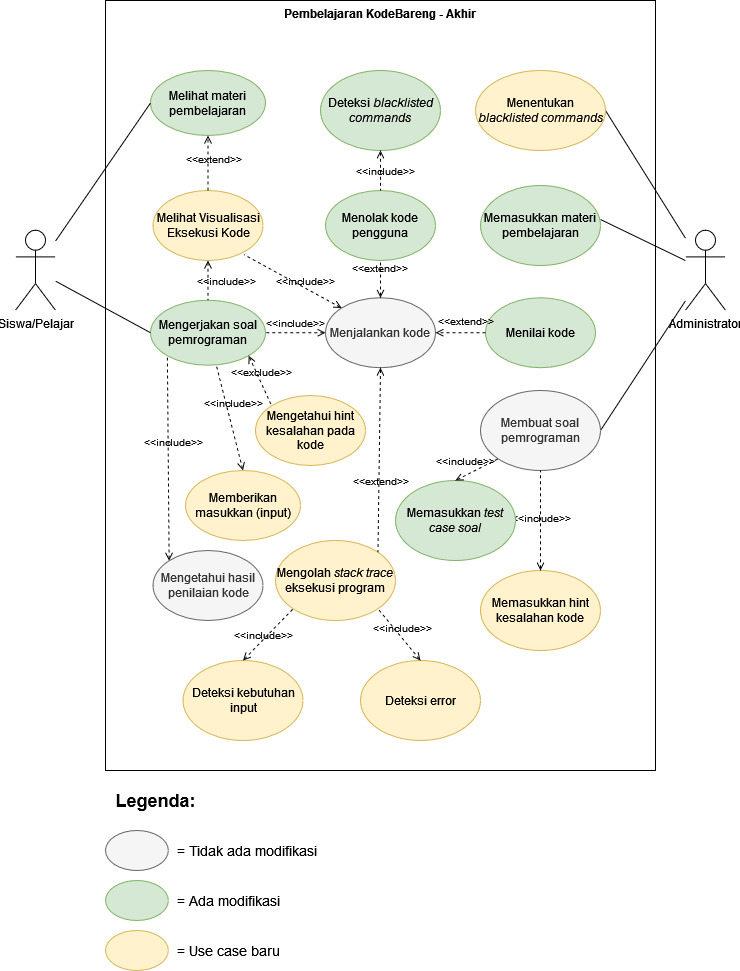
\includegraphics[width=\textwidth]{chapter3/diagram_usecase_v2.jpg}
  \caption{Use Case ILE KodeBareng} \label{fig:diagram-usecase}
\end{figure}

\blindtext

\begin{longtable}[c]{|l|>{\setlength{\baselineskip}{0.75\baselineskip}}p{0.5\linewidth}|>{\setlength{\baselineskip}{0.75\baselineskip}}p{0.3\linewidth}|}
  \caption{Use Case ILE KodeBareng}
  \label{tab:usecase}                                                       \\
  \hline
  \rowcolor{gray!30}
  \textbf{ID} & \textbf{Kebutuhan}                    & \textbf{Penjelasan} \\ \hline
  \endfirsthead
  %
  \endhead
  %
  UC-01       & Melihat materi pembelajaran           &                     \\ \hline
  UC-02       & Mengerjakan soal pemrograman          &                     \\ \hline
  UC-03       & Melihat visualisasi eksekusi kode     &                     \\ \hline
  UC-04       & Mengetahui hasil penilaian kode       &                     \\ \hline
  UC-05       & Memberikan masukkan (input)           &                     \\ \hline
  UC-06       & Mengetahui hint kesalahan pada kode   &                     \\ \hline
  UC-07       & Menjalankan kode                      &                     \\ \hline
  UC-08       & Menolak kode pengguna                 &                     \\ \hline
  UC-09       & Deteksi blacklisted commands          &                     \\ \hline
  UC-11       & Menilai kode                          &                     \\ \hline
  UC-12       & Mengolah stack trace eksekusi program &                     \\ \hline
  UC-13       & Deteksi kebutuhan input               &                     \\ \hline
  UC-14       & Deteksi error                         &                     \\ \hline
  UC-15       & Menentukan blacklisted commands       &                     \\ \hline
  UC-16       & Memasukkan materi pembelajaran        &                     \\ \hline
  UC-17       & Membuat soal pemrograman              &                     \\ \hline
  UC-18       & Memasukkan test case soal             &                     \\ \hline
  UC-19       & Memasukkan hint kesalahan kode        &                     \\ \hline
\end{longtable}

[\hl{TODO: TAMBAHKAN USE CASE DIAGRAMS, DESKRIPSI PROGRAM DIMASUKKAN KESINI, LALU KASIH TABEL KETERKAITAN USECASE DAN REQUIREMENT}]

\begin{longtable}[c]{|l|>{\setlength{\baselineskip}{0.75\baselineskip}}p{0.5\linewidth}|>{\setlength{\baselineskip}{0.75\baselineskip}}p{0.3\linewidth}|}
  \caption{Kebutuhan fungsional sistem}
  \label{tab:fungsional}                                                                                                                                                                                                                                                  \\
  \hline
  \rowcolor{gray!30}
  \textbf{ID} & \textbf{Kebutuhan}                                                                       & \textbf{Penjelasan}                                                                                                                                            \\ \hline
  \endfirsthead
  %
  \endhead
  %
  KB-F-01     & Pengguna memasukkan kode program pada sistem                                             & Menggunakan kakas Monaco Editor                                                                                                                                \\ \hline
  KB-F-02     & Pengguna memasukkan input program pada sistem                                            & Masukan diminta apabila kode membutuhkan masukan                                                                                                               \\ \hline
  KB-F-03     & Pengguna dapat menjalankan kode                                                          & Pengguna dapat melihat hasil eksekusi kode                                                                                                                     \\ \hline
  KB-F-04     & Pengguna dapat melihat hasil visualisasi eksekusi kode                                   & Pengguna dapat melihat perubahan data dan \textit{flow} program yang dijalankan                                                                                \\ \hline
  KB-F-05     & Pengguna mendapat penilaian dari hasil eksekusi kode                                     & Penilaian berdasarkan teknik \textit{blackbox autograding}                                                                                                     \\ \hline
  KB-F-06     & Pengguna mendapat \textit{hint} kesalahan pada kode program                              & -                                                                                                                                                              \\ \hline
  KB-F-07     & Pengguna dapat melihat pesan error pada program                                          & -                                                                                                                                                              \\ \hline
  KB-F-08     & Sistem menolak kode pengguna apabila terdapat perintah-perintah yang tidak diperbolehkan & Keterbatasan eksekusi dapat dilihat disini (TBA)                                                                                                               \\ \hline
  KB-F-09     & Sistem menilai kode program menggunakan \textit{test case}                               & -                                                                                                                                                              \\ \hline
  KB-F-10     & Sistem mengolah \textit{stack trace} eksekusi program                                    & \textit{Stack trace} berisi daftar fungsi, variabel, modul, serta \textit{stack frame} pada tiap langkah eksekusi program. Debugger yang digunakan adalah pdb. \\ \hline
  KB-F-11     & Administrator menentukan perintah-perintah yang tidak diperbolehkan                      & -                                                                                                                                                              \\ \hline
  KB-F-12     & Administrator memasukkan konten materi pembelajaran                                      & Dapat memasukkan visualisasi kode pada materi pembelajaran                                                                                                     \\ \hline
  KB-F-13     & Administrator membuat soal pemrograman                                                   & -                                                                                                                                                              \\ \hline
  KB-F-14     & Administrator memasukkan \textit{test case} soal pemrograman                             & \textit{Test case} tiap soal bisa lebih dari satu dan dapat memiliki input output yang berbeda-beda                                                            \\ \hline
  KB-F-15     & Administrator memasukkan \textit{hint} kesalahan yang dapat ditampilkan pada soal        & -                                                                                                                                                              \\ \hline
\end{longtable}

\blindtext

% Please add the following required packages to your document preamble:
% \usepackage{longtable}
% Note: It may be necessary to compile the document several times to get a multi-page table to line up properly
[\hl{TODO: Pilih 3 aja, performance sama security udah fix}]
\begin{longtable}[c]{|l|l|>{\setlength{\baselineskip}{0.75\baselineskip}}p{0.6\linewidth}|}
  \caption{Kebutuhan non-fungsional sistem}
  \label{tab:non-fungsional}                                                                                       \\
  \hline
  \rowcolor{gray!30}
  \textbf{ID} & \textbf{Parameter} & \textbf{Kebutuhan}                                                            \\ \hline
  \endfirsthead
  %
  \endhead
  %
              & Performance        & Sistem mengembalikan hasil eksekusi paling lama 10 detik                      \\ \hline
              & Reliability        & Sistem menangani 1000 pengguna yang mengerjakan latihan soal secara bersamaan \\ \hline
              & Maintainability    & Implementasi kode sistem menggunakan praktis \textit{clean code}              \\ \hline
              & Testability        & Sistem dirancang sedemikian rupa sehingga mudah dilakukan pengetesan          \\ \hline
              & Security           & Sistem tidak membiarkan terjadinya eksekusi kode berbahaya                    \\ \hline
\end{longtable}
\blindtext

\begin{longtable}[c]{|l|>{\setlength{\baselineskip}{0.75\baselineskip}}p{0.5\linewidth}|}
  \caption{Keterkaitan SRS dan Use Case}
  \label{tab:srs-usecase}                \\
  \hline
  \rowcolor{gray!30}
  \textbf{ID SRS} & \textbf{ID Use Case} \\ \hline
  \endfirsthead
  %
  \endhead
  %
  KB-F-01         & UC-02                \\ \hline
  KB-F-02         & UC-05, UC-13         \\ \hline
  KB-F-03         & UC-02, UC-04, UC-07  \\ \hline
  KB-F-04         & UC-01, UC-02, UC-03  \\ \hline
  KB-F-05         & UC-04, UC-11         \\ \hline
  KB-F-06         & UC-06                \\ \hline
  KB-F-07         & UC-02, UC-14         \\ \hline
  KB-F-08         & UC-08, UC-09         \\ \hline
  KB-F-09         & UC-11                \\ \hline
  KB-F-10         & UC-12                \\ \hline
  KB-F-11         & UC-15                \\ \hline
  KB-F-12         & UC-16                \\ \hline
  KB-F-13         & UC-17                \\ \hline
  KB-F-14         & UC-18                \\ \hline
  KB-F-15         & UC-19                \\ \hline
  KB-NF-01        &                      \\ \hline
  KB-NF-02        &                      \\ \hline
  KB-NF-03        &                      \\ \hline
\end{longtable}

\section{Rancangan Solusi}
 [\hl{TODO: JELASIN LAGI INTERAKTIVITASNYA DIMANA, JELASIN FLOW PROGRAMNYA SEPERTI APA}]

Dalam tugas akhir ini, dibuat prototipe ILE yang terdiri dari beberapa komponen yaitu Web IDE pada \textit{frontend} dan sistem eksekutor kode pada \textit{backend} yang terpisah dari \textit{backend} KodeBareng.

\begin{figure}[H]
  \centering
  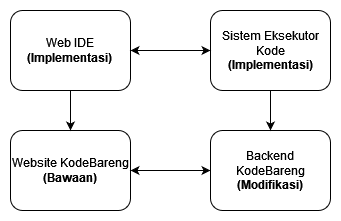
\includegraphics[width=0.5\textwidth]{chapter3/diagram_blok.png}
  \caption{Rancangan Solusi ILE} \label{fig:diagram-blok}
\end{figure}

Keterangan gambar:
\begin{itemize}
  \setlength\itemsep{-0.2cm}
  \item Implementasi: Komponen diimplementasikan dari awal hingga akhir.
  \item Modifikasi: Komponen hanya perlu diubah beberapa bagian.
  \item Bawaan: Komponen tidak berubah.
\end{itemize}

Seperti yang dapat dilihat pada \autoref{fig:diagram-blok} sebelumnya, pada \textit{frontend} akan dibuat komponen Web IDE berupa editor kode yang dapat menerima masukan kode serta memberikan \textit{basic syntax highlighting}. Web IDE dapat menampilkan hasil keluaran ataupun kesalahan eksekusi yang dikembalikan dari \textit{backend}, serta hasil penilaian dari pengetesan kode. Web IDE juga dapat menampilkan visualisasi langkah jalannya program agar dapat memudahkan proses pembelajaran dan pencarian letak masalah dalam implementasi kode.

Pada \textit{backend}, akan dibuat sistem eksekutor kode yang terhubung ke backend KodeBareng. Sistem ini menerima kode dan informasi lainnya dari \textit{backend} lalu melakukan eksekusi kode yang akan dinilai berdasarkan hasil keluarannya. Sistem ini juga dapat terhubung pada \textit{backend} KodeBareng apabila dibutuhkan integrasi lain di kemudian hari.

\subsection{Rancangan Modul}
\autoref{fig:diagram-komponen} Berikut adalah diagram komponen dari sistem yang akan dibuat (TODO: Kalau yang margun udah jadi ntar musti di highlight yg dikerjain yg mana)

\begin{figure}[H]
  \centering
  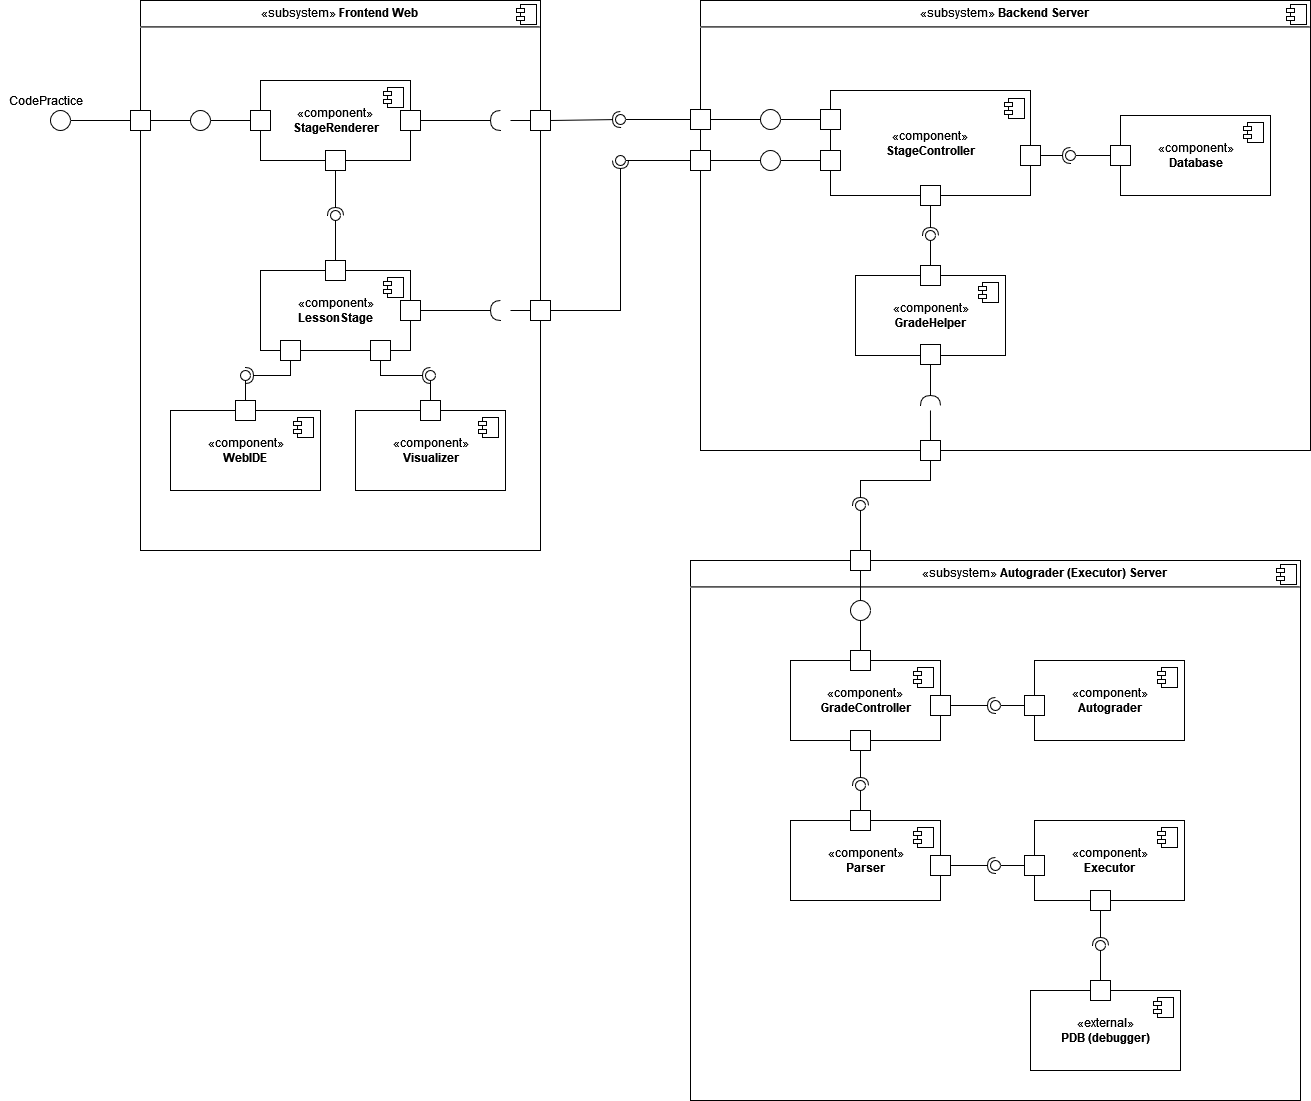
\includegraphics[width=\textwidth]{chapter3/diagram_komponen.png}
  \caption{Diagram komponen} \label{fig:diagram-komponen}
\end{figure}
\blindtext

% \chapter{Implementasi dan Pengujian}

\section{Implementasi}
Berdasarkan hasil analisis serta perancangan yang dituliskan pada Bab III, dilakukan implementasi ILE pada platform web KodeBareng. Dalam bab ini dijelaskan mengenai implementasi dan pengujian terhadap ILE yang dibuat.

\subsection{Batasan Implementasi}
Implementasi dilakukan menggunakan teknologi yang telah dipakai pada KodeBareng sebelumnya. Daftar teknologi dan \textit{framework} yang digunakan pada KodeBareng dapat dilihat pada \autoref{tab:tech-stack}.

\small
\begin{longtable}[c]{|>{\setlength{\baselineskip}{0.75\baselineskip}}p{0.3\linewidth}|>{\setlength{\baselineskip}{0.75\baselineskip}}p{0.4\linewidth}|}
  \caption{\textit{Tech stack} yang digunakan oleh KodeBareng} \label{tab:tech-stack}                               \\ \hline
  \rowcolor{gray!30}
  \textbf{Nama Sistem}                                     & \textbf{Teknologi / \textit{Framework} yang digunakan} \\ \hline
  \endfirsthead
  %
  \caption*{\autoref{tab:tech-stack} (lanjutan): \textit{Tech stack} yang digunakan oleh KodeBareng}                \\ \hline
  \rowcolor{gray!30}
  \textbf{Nama Sistem}                                     & \textbf{Teknologi / \textit{Framework} yang digunakan} \\ \hline
  \endhead
  %
  \textit{Frontend}                                        & NuxtJS, Cloudflare Pages                               \\ \hline
  \textit{Backend}                                         & ExpressJS, Linux, NodeJS, Docker                       \\ \hline
  CMS (\textit{Content Management System})                 & NextJS, Netlify                                        \\ \hline
  \textit{Autograder} (sekarang menjadi \textit{Executor}) & ExpressJS, Linux, NodeJS, Docker, Python 3.9           \\ \hline
\end{longtable}
\normalsize

Selain dari teknologi yang digunakan, terdapat juga batasan dari bahasa pemrograman yang dapat divisualisasikan eksekusinya yaitu Python sesuai dengan kelas pembelajaran pemrograman yang sudah ada pada platform web KodeBareng.

\footnotesize
\begin{longtable}[c]{|l|l|}
  \caption{Cakupan implementasi ILE} \label{tab:ile-scope}                      \\ \hline
  \rowcolor{gray!30}
  \small\textbf{Concepts}                       & \small Termasuk Implementasi? \\ \hline
  \endfirsthead
  %
  \caption*{\autoref{tab:ile-scope} (lanjutan): Cakupan implementasi ILE}       \\ \hline
  \rowcolor{gray!30}
  \small\textbf{Concepts}                       & \small Termasuk Implementasi? \\ \hline
  \endhead
  %
  \textbf{Input/Output}                         &                               \\ \hline
  Standard Input/Output                         & Termasuk                      \\ \hline
  File I/O                                      & Tidak Termasuk                \\ \hline
  \textbf{Variables}                            &                               \\ \hline
  Variable types                                & Termasuk                      \\ \hline
  Variable scope                                & Termasuk                      \\ \hline
  Assignment of values to variables             & Termasuk                      \\ \hline
  \textbf{Selection and repetition structures}  &                               \\ \hline
  If statement                                  & Termasuk                      \\ \hline
  While loop                                    & Termasuk                      \\ \hline
  For loop                                      & Termasuk                      \\ \hline
  \textbf{Methods}                              &                               \\ \hline
  Method structure                              & Termasuk                      \\ \hline
  Method frames                                 & Termasuk                      \\ \hline
  Message passing                               & Termasuk                      \\ \hline
  Return values                                 & Termasuk                      \\ \hline
  Recursion                                     & Termasuk                      \\ \hline
  Lambda function                               & Tidak Termasuk                \\ \hline
  \textbf{Arrays}                               &                               \\ \hline
  Arrays as objects                             & Termasuk                      \\ \hline
  Array structure                               & Termasuk                      \\ \hline
  Arrays of primitives                          & Termasuk                      \\ \hline
  Arrays of references                          & Tidak Termasuk                \\ \hline
  Array index                                   & Termasuk                      \\ \hline
  List Comprehension                            & Tidak Termasuk                \\ \hline
  \textbf{Algorithms}                           &                               \\ \hline
  Search algorithms                             & Tidak Termasuk                \\ \hline
  Sort algorithms                               & Tidak Termasuk                \\ \hline
  Data structures (linked list and binary tree) & Tidak Termasuk                \\ \hline
  \textbf{Additional requirements}              &                               \\ \hline
  Debugging                                     & Tidak Termasuk                \\ \hline
  Standard libraries                            & Termasuk                      \\ \hline
\end{longtable}
\normalsize

\subsection{Implementasi Sistem Eksekutor}
% [\hl{TODO: MASUKIN INPUT, PROSES, OUTPUT MASING2 KOMPONEN}]
% [\hl{TODO: MASUKIN KOMPONEN/LIBRARY YANG DIGUNAKNA UNTUK TIAP KOMPONEN}]
% [\hl{TODO: MASUKIN TREE VIEW TIAP KOMPONEN LETAKNYA ADA DIMANA AJA}]
% [\hl{TODO: MASUKIN HAMBATAN DAN SOLUSI DI TIAP KOMPONEN}]

Sistem Eksekutor menggunakan \textit{tech stack} berupa ExpressJS dengan Typescript yang dijalankan pada NodeJS menggunakan kakas \textit{nodemon}. Sistem tersebut kemudian diisolasi menggunakan Docker dengan \textit{image} Debian 10 dan dilakukan instalasi Python 3.9. Terdapat juga kakas berupa \textit{swagger} yang digunakan untuk dokumentasi rute-rute yang terdapat pada sistem ini.

\subsubsection{Modifikasi Komponen Controller}
Pada sistem ini sudah terdapat \textit{controller} pada tiap bagian rute untuk mengolah data yang diberikan. Pada Tugas Akhir ini, ditambahkan rute untuk melakukan visualisasi serta \textit{controller} untuk mengolah data tersebut. \textit{Controller} mendapatkan masukan berupa kode program berupa \textit{string} serta input berupa \verb|array of string| untuk diberikan pada program yang dieksekusi. Kemudian, \textit{Controller} melakukan pengecekan apakah kode diperbolehkan untuk dieksekusi, lalu menuliskan kode pada file Python sementara. Setelah itu, \textit{controller} menjalankan \textit{helper} berupa Komponen Executor dan Parser dengan memberikan masukan berupa lokasi \textit{file} kode program serta \textit{input} yang akan diberikan pada program.

% [\hl{TODO: MASUKIN CONTOH HASIL INPUT CONTROLLER UNTUK KOMPONEN EXECUTOR DAN PARSER}]

\subsubsection{Implementasi Komponen Executor}
Komponen Executor merupakan komponen yang digunakan untuk mengeksekusi kode program menggunakan PDB. Komponen ini membutuhkan masukan berupa lokasi \textit{file} berisi kode program yang akan dieksekusi serta \textit{input} yang akan diberikan kepada program. Terdapat 3 tahapan utama dalam komponen ini, yaitu tahap inisialisasi, tahap pengecekan, serta tahap pengumpulan data.

Tahap inisialisasi adalah tahap menginjeksi kode tambahan ke dalam eksekusi Python untuk keperluan Komponen Executor dan Parser. Pada tahap ini, dimasukkan kode untuk mengubah keluaran Python menjadi JSON agar dapat diolah oleh NodeJS. Selain itu, terdapat juga fungsi-fungsi tambahan untuk mendapatkan tipe data pada Python serta melakukan \textit{deep iteration} untuk mendapatkan informasi tipe data serta id dari variabel yang bertipe \textit{sequence} atau \textit{hashmap}. Tahap inisialisasi hanya dilakukan sekali untuk setiap kode program yang dijalankan.

Setelah inisialisasi dijalankan, dilakukan tahap pengecekan yaitu untuk mengecek apakah eksekusi program sedang berada di luar kode program yang seharusnya karena terkadang PDB menjalankan kode program pada modul \textit{standard library} (\textit{built-in module}). Apabila program sedang mengeksekusi baris diluar kode program (penentuan dilakukan oleh Komponen Parser), maka Komponen Executor akan mengeksekusi perintah untuk kembali keluar modul tersebut dan kembali pada kode program awal. Setelah itu, Komponen Executor akan melanjutkan langkah eksekusi tanpa melalui tahapan pengumpulan data.

Apabila program lolos dari tahap pengecekan (program tidak berada di luar kode program), maka dilakukan tahap pengumpulan data. Tahap pengumpulan data adalah tahap pengumpulan \textit{fields} yang berada pada \textit{runtime memory} seperti variabel, fungsi dan metode, serta modul yang telah dimuat. Tahap ini terbagi menjadi 3 subtahap, yaitu tahap \verb|Local|, \verb|Global|, dan \verb|Stack|. Subtahap \verb|Lokal| adalah subtahap mengeksekusi perintah untuk mengumpulkan \textit{fields} pada memori lokal suatu \textit{stack frame}. Subtahap \verb|Global| adalah subtahap mengeksekusi perintah untuk mengumpulkan \textit{fields} pada memori global suatu program. Subtahap \verb|Stack| adalah subtahap mengeksekusi perintah untuk mengumpulkan data pada \textit{stack frame} berupa baris kode yang sedang dieksekusi, \textit{return value}, serta daftar \textit{frame} yang tersimpan pada \textit{stack frame}.Hasil keluaran dari seluruh perintah tersebut akan diolah oleh Komponen Parser.

Setelah Komponen Executor dan Parser melewati tahap pengumpulan data dan tidak terjadi error, maka Komponen Executor akan melanjutkan langkah eksekusi kode sekaligus perintah yang digunakan untuk pengecekan \textit{error}, serta me-\textit{reset} data-data dan tahapan-tahapan yang dilakukan lalu kembali pada tahap pengecekan. Apabila terdapat error selama tahap pengumpulan data, maka Komponen Executor akan mematikan program yang sedang dieksekusi. Apabila jumlah langkah atau lama waktu eksekusi sudah melebihi batas yang telah ditentukan, maka Komponen Executor juga akan mematikan program yang sedang dieksekusi.

% [\hl{TODO: MASUKIN CONTOH HASIL KELUARAN KOMPONEN EXECUTOR }]

\subsubsection{Implementasi Komponen Parser}
Komponen Parser merupakan komponen yang digunakan untuk mengolah hasil keluaran Komponen Executor. Komponen ini juga menentukan logika dan langkah yang akan diambil oleh Komponen Executor. Komponen ini membutuhkan masukan berupa \verb|array of string| yang merupakan hasil keluaran Komponen Executor yang telah dipisahkan tiap barisnya. Terdapat 2 tahapan utama dalam komponen ini, yaitu tahap pengecekan dan tahap pengumpulan data.

Tahap pengecekan dilakukan bersamaan dengan Komponen Executor melakukan tahap pengecekan. Pada tahap ini, terdapat beberapa subtahap yaitu pengecekan \textit{input}, pengecekan \textit{output}, serta pengecekan eksekusi \textit{built-in module}.

Pada subtahap pengecekan \textit{input}, dilakukan pengecekan terhadap \textit{signature output} dari PDB serta pengecekan waktu eksekusi suatu baris. Apabila tidak ditemukan \textit{signature output} dari PDB atau waktu eksekusi suatu baris melebihi batas, maka komponen ini akan memasukkan \textit{input} (melalui Komponen Executor) sesuai dengan \textit{input} yang dberikan oleh \textit{controller}. Apabila tidak ada \textit{input} yang diberikan oleh \textit{controller} atau \textit{input} yang diberikan oleh \textit{controller} kurang dari jumlah input yang dibutuhkan, maka Komponen Parser akan memasukkan \textit{event} untuk meminta tambahan input dan mematikan program yang dieksekusi.

Setelah itu, dilakukan subtahap pengecekan \textit{output} untuk mengecek dan mengolah apabila program mengeluarkan \textit{output} atau \textit{error} setelah melanjutkan langkah eksekusi. Apabila program mengeluarkan \textit{error}, maka Komponen Parser akan mengolah \textit{error} dan \textit{traceback} yang dikeluarkan dan menyimpannya ke dalam \textit{event} lalu mematikan program. Apabila program mengeluarkan \textit{output}, maka Komponen Parser akan mengolah \textit{output} tersebut dan memasukkannya ke dalam daftar \textit{output} program.

Kemudian, dilakukan subtahap pengecekan eksekusi \textit{built-in module} yang telah dijelaskan pada Komponen Executor sebelumnya. Komponen Parser akan mengecek hasil keluaran dari perintah yang dimasukkan oleh Komponen Executor, kemudian apabila terdeteksi \textit{error} maka Komponen Parser tidak akan mengolah data hingga Komponen Executor melanjutkan langkah eksekusi program.

Setelah seluruh tahapan dalam tahap pengecekan selesai, Komponen Parser akan memasuki tahap pengumpulan data yang tahapannya sama dengan tahapan pengumpulan data yang terdapat pada Komponen Executor. Hasil keluaran Komponen Executor diolah dengan mengolah keluaran JSON. Apabila keluaran tersebut tidak dapat diolah sebagai JSON, maka Komponen Parser akan menghasilkan \textit{error}, disimpan sebagai \textit{event} lalu mematikan program. Setelah semua subtahap pengumpulan data dilakukan, Komponen Parser akan mengolah seluruh hasil pengumpulan data ke dalam daftar \verb|ExecutionResult| yang akan dikembalikan kepada \textit{controller} saat program telah selesai atau dimatikan dan menjadi hasil yang dapat divisualisasikan pada Sistem Frontend.

% [\hl{TODO: MASUKKAN CONTOH HASIL KELUARAN KOMPONEN PARSER}]

\subsection{Implementasi Backend}
\subsubsection{Implementasi Komponen Helper}
Komponen Helper merupakan komponen yang digunakan untuk mendeteksi perintah-perintah yang tidak diperbolehkan eksekusi pada kode. Apabila tidak terdapat perintah yang dilarang pada kode, maka kode diteruskan kepada sistem Executor dan mengembalikan hasilnya. Apabila terdapat perintah yang dilarang pada kode, maka kode akan ditolak dan tidak akan dieksekusi.


\subsection{Implementasi Frontend}

\subsubsection{Implementasi Komponen Web IDE}
Komponen Web IDE dibuat menggunakan Monaco Editor yang dibuat oleh Microsoft. Komponen ini dapat memperlihatkan \textit{syntax highlighting} pada kode, menunjukkan angka baris, serta navigasi menggunakan \textit{scrollbar} yang memiliki \textit{overview} dari seluruh kode program.

Komponen ini terhubung pada Komponen Visualizer untuk menampilkan dekorator-dekorator saat visualisasi eksekusi kode berlangsung. Tampilan hasil implementasi Web IDE dapat dilihat pada \autoref{fig:web-ide}.

\begin{figure}[H]
  \centering
  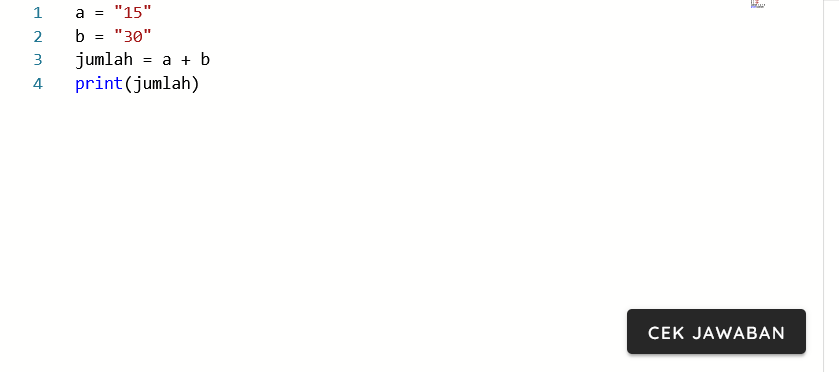
\includegraphics[width=0.7\textwidth]{chapter4/web-ide.png}
  \caption{Tampilan Antarmuka Web IDE \\ Sumber: Penulis (2022)} \label{fig:web-ide}
\end{figure}

\subsubsection{Implementasi Komponen Visualizer}
Komponen Visualizer merupakan komponen yang dapat memvisualisasikan hasil olahan \textit{stack trace} suatu kode. Komponen ini dapat berinteraksi dengan Web IDE untuk menunjukkan lokasi eksekusi suatu langkah dengan memberikan warna pada baris eksekusi, serta membuat tabel data pada memori pada setiap \textit{stack frame}. Pengguna dapat mengubah alur maju mundur visualisasi, melihat isi data pada setiap \textit{stack frame}, serta melihat perubahan pada data dalam memori.

Komponen ini dapat dimasukkan pada bagian materi pembelajaran dan bagian persoalan seperti Kuis dan Latihan Kode. Komponen ini dapat dinon-aktifkan apabila tidak diperbolehkan untuk digunakan. Tampilan hasil implementasi Visualizer dapat dilihat pada \autoref{fig:ile-materi} dan \autoref{fig:ile-soal}.

\begin{figure}[H]
  \centering
  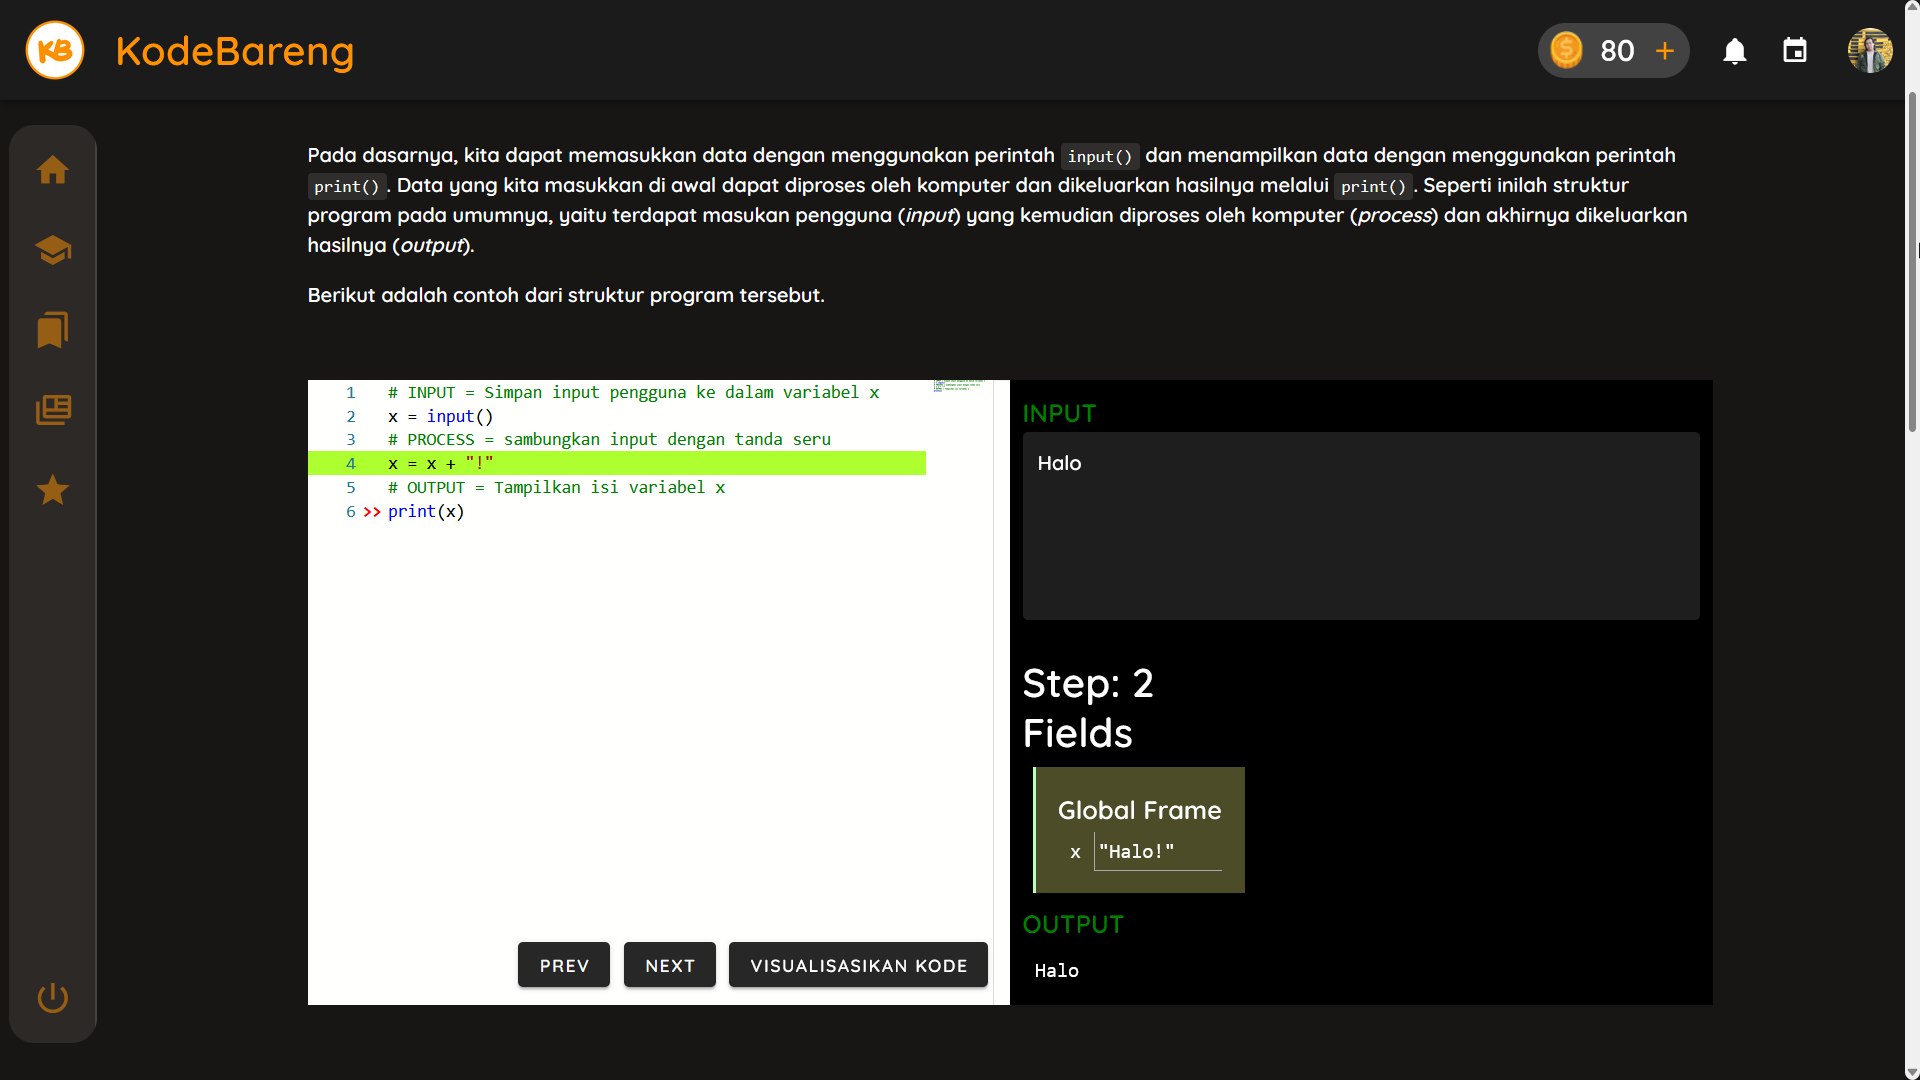
\includegraphics[width=0.7\textwidth]{chapter4/ile-materi.png}
  \caption{Tampilan antarmuka Visualizer pada materi pembelajaran \\ Sumber: Penulis (2022)} \label{fig:ile-materi}
\end{figure}
\begin{figure}[H]
  \centering
  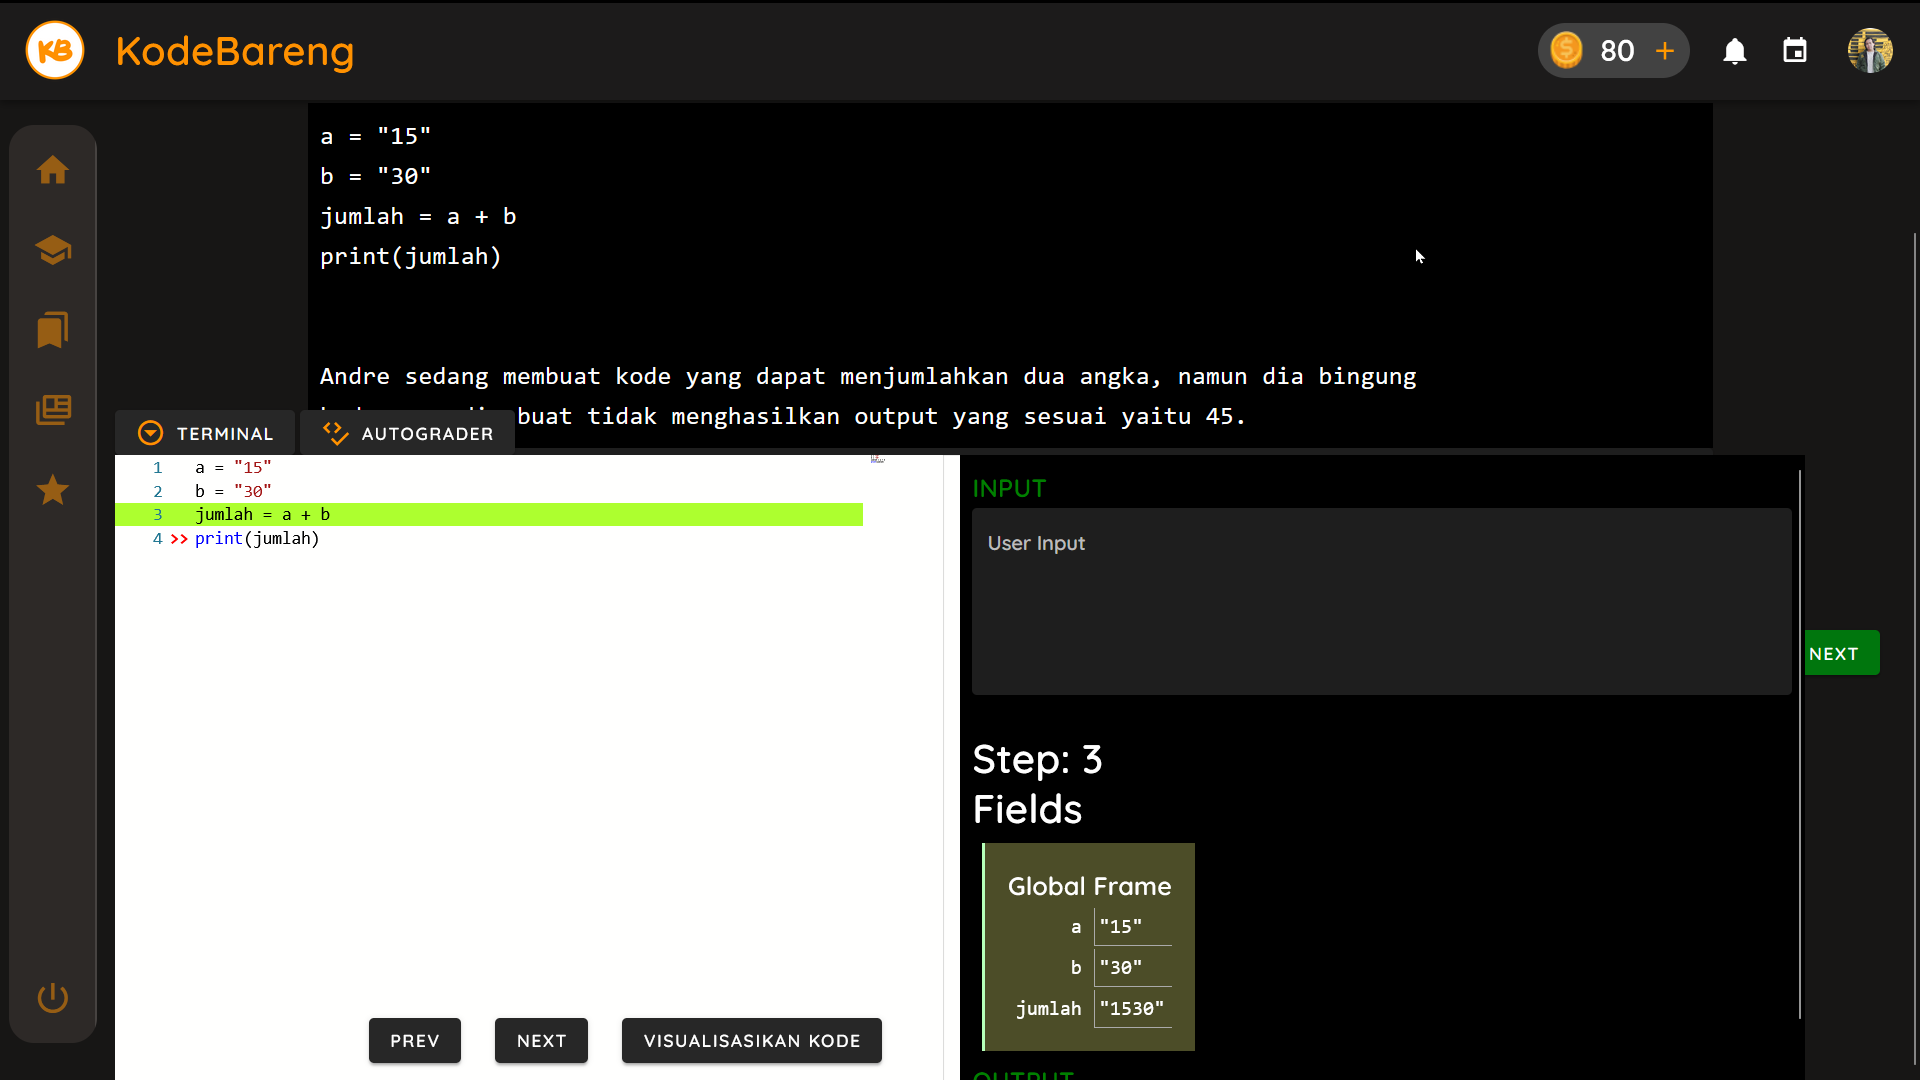
\includegraphics[width=0.7\textwidth]{chapter4/ile-soal.png}
  \caption{Tampilan antarmuka Visualizer pada persoalan Latihan Kode \\ Sumber: Penulis (2022)} \label{fig:ile-soal}
\end{figure}

\section{Pengujian}

\subsection{Tujuan Pengujian}
Tujuan dari pengujian ini adalah untuk memastikan bahwa ILE yang diimplementasikan telah sesuai dengan spesifikasi kebutuhan yang telah dibuat sebelumnya serta mendapatkan data terkait dampak ILE yang telah dibuat terhadap pemahaman pelajar mengenai konsep serta alur kerja eksekusi kode program.

\subsection{Lingkungan Pengujian}
Lingkungan pengujian terbagi menjadi 2 yaitu lingkungan komputer dan lingkungan eksperimen pengguna (\textit{user experiment}). Lingkungan komputer digunakan untuk menjalankan fungsional sistem, sementara lingkungan eksperimen pengguna digunakan untuk melakukan eksperimen pengguna pada komputer peserta eksperimen masing-masing.

Pengujian spesifikasi fungsional sistem dilakukan pada komputer server KodeBareng dengan spesifikasi pada \autoref{tab:lingkungan-server} untuk menjalankan Sistem Backend dan Sistem Executor.

\small
\begin{longtable}[c]{|l|l|}
  \caption{Lingkungan pengujian komputer server} \label{tab:lingkungan-server}                \\ \hline
  \rowcolor{gray!30}
  \textbf{Komponen} & \textbf{Keterangan}                                                     \\ \hline
  \endfirsthead
  %
  \caption*{\autoref{tab:lingkungan-server} (lanjutan): Lingkungan pengujian komputer server} \\ \hline
  \rowcolor{gray!30}
  \textbf{Komponen} & \textbf{Keterangan}                                                     \\ \hline
  \endhead
  %
  Prosesor          & Intel(R) Xeon(R) CPU E5-2660 0 @ 2.20GHz                                \\ \hline
  Memori            & 2GB                                                                     \\ \hline
  Storage           & 32GB                                                                    \\ \hline
  Sistem Operasi    & Ubuntu 20.04.4 LTS                                                      \\ \hline
\end{longtable}
\normalsize

Eksperiment pengguna dilakukan pada komputer peserta eksperimen masing-masing secara daring dengan pengarahan menggunakan platform \textit{Google Meet}.

\subsection{Skenario dan Hasil Pengujian}

\subsubsection{Pengujian Fungsional}
Pengujian fungsional dilakukan berdasarkan spesifikasi kebutuhan fungsional dan non-fungsional ILE pada \autoref{tab:srs-fungsional} dan \autoref{tab:srs-nonfungsional} pada \autoref{sec:analisis-kebutuhan}. Skenario dan hasil pengujian dapat dilihat pada \autoref{tab:pengujian-fungsional} dan \autoref{tab:pengujian-nonfungsional} berikut.

\small
\begin{longtable}[c]{|l|>{\setlength{\baselineskip}{0.75\baselineskip}}p{0.5\linewidth}|>{\setlength{\baselineskip}{0.75\baselineskip}}p{0.2\linewidth}|}
  \caption{Skenario dan hasil pengujian fungsional} \label{tab:pengujian-fungsional}                                     \\ \hline
  \rowcolor{gray!30}
  \textbf{ID} & \textbf{Skenario}                                                                       & \textbf{Hasil} \\ \hline
  \endfirsthead
  %
  \caption*{\autoref{tab:pengujian-fungsional} (lanjutan): Skenario dan hasil pengujian fungsional}                      \\ \hline
  \rowcolor{gray!30}
  \textbf{ID} & \textbf{Skenario}                                                                       & \textbf{Hasil} \\ \hline
  \endhead
  %
  KB-F-01     & Pelajar memasukkan kode program pada sistem                                             & Diterima       \\ \hline
  KB-F-02     & Pelajar memasukkan input program pada sistem                                            & Diterima       \\ \hline
  KB-F-03     & Pelajar dapat menjalankan kode                                                          & Diterima       \\ \hline
  KB-F-04     & Pelajar dapat melihat hasil visualisasi eksekusi kode                                   & Diterima       \\ \hline
  KB-F-05     & Pelajar mendapat penilaian dari hasil eksekusi kode                                     & Diterima       \\ \hline
  KB-F-06     & Pelajar mendapat \textit{hint} kesalahan pada kode program                              & Diterima       \\ \hline
  KB-F-07     & Pelajar dapat melihat pesan error pada program                                          & Diterima       \\ \hline
  KB-F-08     & Sistem menolak kode pelajar apabila terdapat perintah-perintah yang tidak diperbolehkan & Diterima       \\ \hline
  KB-F-09     & Sistem menilai kode program menggunakan \textit{test case}                              & Diterima       \\ \hline
  KB-F-10     & Sistem mengolah \textit{stack trace} eksekusi program                                   & Diterima       \\ \hline
  KB-F-11     & Administrator menentukan perintah-perintah yang tidak diperbolehkan                     & Diterima       \\ \hline
  KB-F-12     & Administrator memasukkan konten materi pembelajaran                                     & Diterima       \\ \hline
  KB-F-13     & Administrator membuat soal pemrograman                                                  & Diterima       \\ \hline
  KB-F-14     & Administrator memasukkan \textit{test case} soal pemrograman                            & Diterima       \\ \hline
  KB-F-15     & Administrator memasukkan \textit{hint} kesalahan yang dapat ditampilkan pada soal       & Diterima       \\ \hline
\end{longtable}
\normalsize

\small
\begin{longtable}[c]{|l|>{\setlength{\baselineskip}{0.75\baselineskip}}p{0.6\linewidth}|l|}
  \caption{Skenario dan hasil pengujian non-fungsional} \label{tab:pengujian-nonfungsional}                \\ \hline
  \rowcolor{gray!30}
  \textbf{ID} & \textbf{Skenario}                                         & \textbf{Hasil}                 \\ \hline
  \endfirsthead
  %
  \caption*{\autoref{tab:pengujian-nonfungsional} (lanjutan): Skenario dan hasil pengujian non-fungsional} \\ \hline
  \rowcolor{gray!30}
  \textbf{ID} & \textbf{Skenario}                                         & \textbf{Hasil}                 \\ \hline
  \endhead
  %
  KB-NF-01    & Sistem mengembalikan hasil eksekusi paling lama 10 detik. & Diterima                       \\ \hline
  KB-NF-02    & Sistem dapat diuji menggunakan beragam kode program       & Diterima                       \\ \hline
  KB-NF-03    & Sistem menolak kode berbahaya                             & Diterima                       \\ \hline
\end{longtable}
\normalsize

\subsubsection{Eksperimen Pengguna (\textit{User Experiment})}

Eksperimen pengguna dilakukan terhadap faktor pemahaman pelajar mengenai konsep pemrograman serta alur kerja eksekusi kode program. Maka dari itu, pengujian dilakukan berdasarkan pengujian pada \textcite{mayer1981psychology} untuk perlakuan pemberian model konkret kepada pelajar saat pembelajaran berlangsung serta \textcite{moons2013pilot} untuk cara pengukuran pemahaman konsep. Sebagai batasan, eksperimen ini hanya akan dilakukan pada orang yang baru belajar pemrograman atau belum pernah belajar pemrograman sebelumnya.

Pengujian ini dilakukan pada platform web KodeBareng dengan menggunakan kelas pembelajaran khusus untuk melakukan pengujian. Pengujian dilakukan pada 2 grup dengan masing-masing grup memiliki minimal 10 peserta eksperimen, yaitu grup kontrol dan grup perlakuan. Grup kontrol mendapatkan materi pembelajaran tanpa adanya integrasi ILE visualisasi eksekusi kode, sementara grup perlakuan mendapatkan materi pembelajaran yang terdapat integrasi ILE visualisasi eksekusi kode. Setiap grup mendapatkan materi pembelajaran yang sama serta kuesioner setelah melakukan pembelajaran.

Materi yang diberikan terbagi menjadi 3 modul yaitu modul Pengenalan Python Dasar, Variabel dan Tipe Data, serta Operator dan Ekspresi. Pada masing-masing modul, terdapat 2 tahapan yaitu tahap pembelajaran dan tahap persoalan. Pada tahap pembelajaran, materi diberikan melalui teks, gambar dan ILE (khusus pada grup perlakuan, pada grup kontrol hanya diperlihatkan teks kode serta \textit{input/output}-nya). Pada tahap persoalan, terdapat 2 jenis persoalan yaitu kuis dan latihan kode. Soal kuis adalah soal sederhana bertipe pilihan ganda, sementara soal latihan kode adalah soal yang memberikan bagian suatu kode program yang harus diubah oleh peserta untuk memenuhi objektif yang diberikan. Soal kuis dinilai secara benar atau salah (1/0) dan soal latihan kode akan dinilai menggunakan SOLO Level dengan kategori penilaian seperti pada \autoref{tab:solo-level} namun hanya mencapai level ke-4 karena pembelajaran tidak sampai diujikan pada domain lainnya. SOLO (Structure of Observed Learning Outcomes) adalah salah satu jenis taksonomi dalam pendidikan yang mengukur tingkat abstraksi pemahaman konsep yang telah dicapai oleh peserta didik \parencite{moons2013pilot}. Pada setiap akhir modul, terdapat 2 soal kuis dan 1 soal latihan kode. Setiap tahapan harus diselesaikan terlebih dahulu sebelum peserta dapat melanjutkan pembelajaran.

Pada kuesioner, terdapat 2 pertanyaan menggunakan \textit{likert scale} yaitu "Apakah visualisasi kode membuatmu lebih memahami kode yang dijalankan?" dan "Apakah visualisasi kode membantumu menjawab kuis dan latihan soal?", serta 1 pertanyaan bertipe isian paragraf yaitu "Pendapat atau saran untuk fitur visualisasi eksekusi kode". Selain pertanyaan yang berkaitan dengan ILE, terdapat juga pertanyaan umum lainnya seperti pengalaman pembelajaran di KodeBareng dan pendapat saran untuk pembelajaran di KodeBareng. Kuesioner digunakan sebagai data kualitatif tambahan untuk mengukur dampak dari ILE dari sisi penggunanya. Pertanyaan kuesioner terkait ILE hanya dijawab oleh peserta grup perlakuan.

Selain dari materi pembelajaran dan kuesioner, terdapat juga data tambahan berupa \textit{event} yang disimpan selama eksperimen berlangsung untuk mengukur waktu pembelajaran pada suatu tahap, berapa banyak interaksi yang dilakukan pelajar pada ILE, serta jawaban-jawaban yang di-\textit{submit} oleh pelajar saat menjawab persoalan Kuis dan Latihan Kode.

\subsection{Prosedur Eksperimen Pengguna}
Sebelum pengujian, disebarkan formulir pendaftaran eksperimen yang dilakukan pada Sabtu, 28 Mei 2022. Selain data kontak dan demografis, data mengenai pengalaman pembelajaran pemrograman sebelumnya juga diambil. Pengujian dilakukan dalam rentan waktu 4 hari, yaitu dimulai pada 29 Mei hingga 1 Juni 2022. Orang yang telah mendaftar eksperimen kemudian dikontak untuk dilakukan penjadwalan eksperimen. Dari 42 orang yang mendaftar eksperimen melalui formulir tersebut, terdapat 25 orang yang merespon dan dapat menjadwalkan eksperimen sehingga menjadi peserta eksperimen yang sah. Demografis peserta eksperimen dapat dilihat pada \autoref{fig:demografis-usia}, \autoref{fig:demografis-pendidikan}, serta \autoref{fig:demografis-kelamin}. Kemudian, peserta dipetakan menjadi 13 orang grup perlakuan dan 12 orang grup kontrol.

\begin{figure}[H]
  \centering
  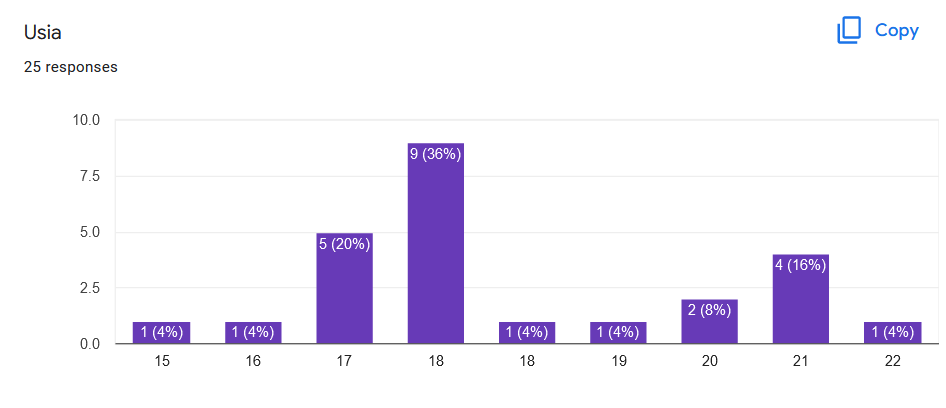
\includegraphics[width=0.7\textwidth]{chapter4/demografis-usia.png}
  \caption{Demografis usia peserta eksperimen \\ Sumber: Penulis (2022)} \label{fig:demografis-usia}
\end{figure}
\begin{figure}[H]
  \centering
  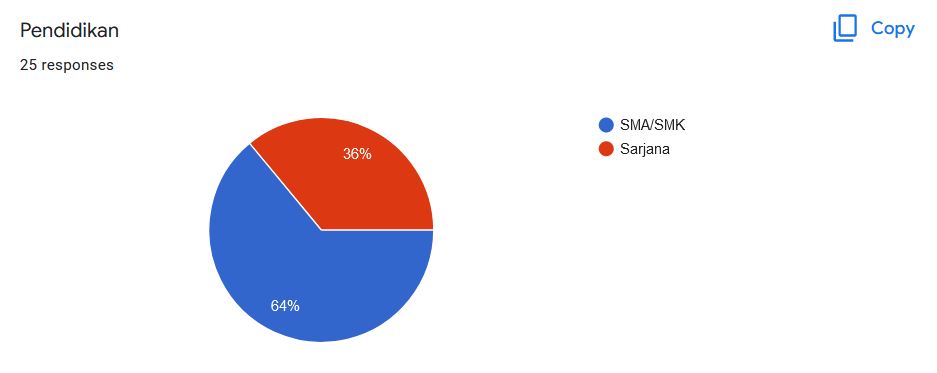
\includegraphics[width=0.7\textwidth]{chapter4/demografis-pendidikan.png}
  \caption{Demografis tahap pendidikan peserta eksperimen \\ Sumber: Penulis (2022)} \label{fig:demografis-pendidikan}
\end{figure}
\begin{figure}[H]
  \centering
  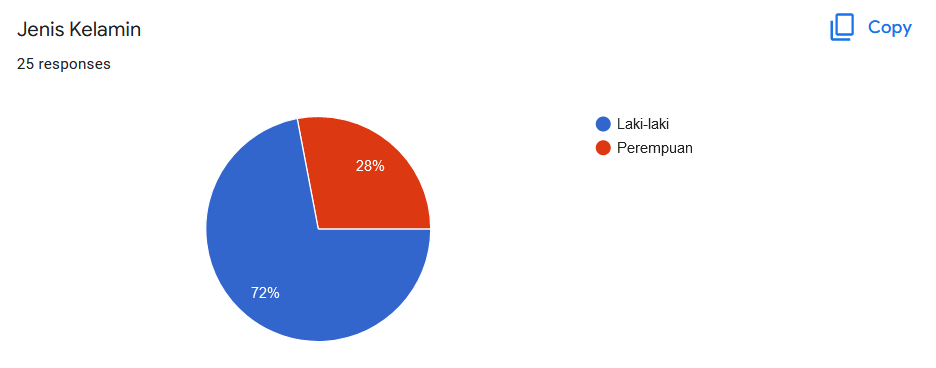
\includegraphics[width=0.7\textwidth]{chapter4/demografis-kelamin.png}
  \caption{Demografis jenis kelamin peserta eksperimen \\ Sumber: Penulis (2022)} \label{fig:demografis-kelamin}
\end{figure}

Eksperimen dilakukan secara daring menggunakan platform \textit{Google Meet}. Peserta dibagikan tautan \textit{Google Meet} sesuai dengan jadwal kloter eksperimen yang sudah ditentukan sebelumnya. Peserta diminta menggunakan laptop/komputer saat melakukan eksperimen. Setelah seluruh peserta dalam satu kloter telah masuk ke dalam \textit{Google Meet}, peserta dibagikan tautan menuju formulir kuesioner untuk mengisi identitas diri terlebih dahulu. Kemudian, peserta diarahkan menuju situs KodeBareng, membuat akun KodeBareng menggunakan akun Google, lalu membuka kelas sesuai dengan grup masing-masing. Sebelum memulai pembelajaran, peserta diberikan arahan mengenai cara belajar di KodeBareng serta instruksi untuk melakukan pembelajaran sesuai dengan kecepatan masing-masing selama 1 jam. Khusus untuk peserta pada grup perlakuan, mereka diberikan pengenalan cara menggunakan ILE yang telah disediakan selama pembelajaran. Setelah 1 jam berlalu, selesai tidak selesai peserta akan diminta untuk menghentikan pembelajaran lalu melanjutkan mengisi kuesioner.

\section{Analisis Hasil Pengujian} \label{sec:analisis-hasil-pengujian}

\subsection{Analisis Data Kuesioner}
Karena pertanyaan kuesioner hanya diberikan kepada peserta yang telah memakai ILE, terdapat 13 peserta yang memberikan respon terhadap pertanyaan kuesioner. Terdapat 2 pertanyaan kuesioner yang diberikan, yaitu pertanyaan untuk mengukur dampak ILE terhadap pemahaman kode yang dijalankan serta pertanyaan untuk mengukur dampak ILE terhadap penyelesaian soal kuis dan latihan kode.

Berikut \autoref{fig:kuesioner-memahami} dan \autoref{tab:kuesioner1-statistik} adalah grafik serta tabel perhitungan statistik dari pertanyaan kuesioner pertama.

\begin{figure}[H]
  \centering
  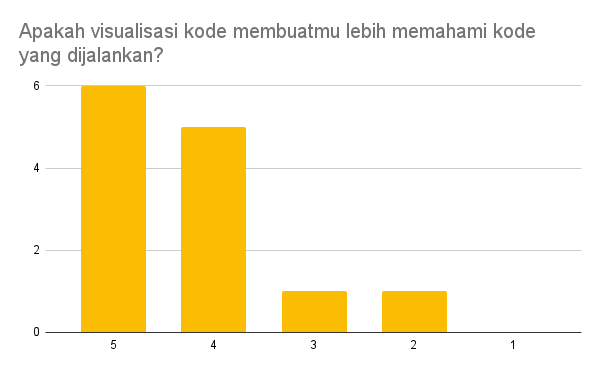
\includegraphics[width=0.7\textwidth]{chapter4/kuesioner-memahami.png}
  \caption{Apakah ILE membantu memahami kode? \\ Sumber: Penulis (2022)} \label{fig:kuesioner-memahami}
\end{figure}

\small
\begin{longtable}[c]{|l|>{\setlength{\baselineskip}{0.75\baselineskip}}p{0.5\linewidth}|}
  \caption{Hasil perhitungan statistik deskriptif pada respon kuesioner pertanyaan pertama} \label{tab:kuesioner1-statistik}                                                 \\ \hline
                           & Apakah visualisasi kode membuatmu lebih memahami kode yang dijalankan?                                                                          \\ \hline
  \endfirsthead
  %
  \caption*{\autoref{tab:kuesioner1-statistik} (lanjutan): Hasil perhitungan statistik deskriptif pada respon kuesioner pertanyaan pertama} \label{tab:kuesioner1-statistik} \\ \hline
                           & Apakah visualisasi kode membuatmu lebih memahami kode yang dijalankan?                                                                          \\ \hline
  \endhead
  %
  Mean                     & 4.230769                                                                                                                                        \\ \hline
  Standard Error           & 0.25705                                                                                                                                         \\ \hline
  Median                   & 4                                                                                                                                               \\ \hline
  Mode                     & 5                                                                                                                                               \\ \hline
  Standard Deviation       & 0.926809                                                                                                                                        \\ \hline
  Sample Variance          & 0.858974                                                                                                                                        \\ \hline
  Kurtosis                 & 1.524332                                                                                                                                        \\ \hline
  Skewness                 & -1.27368                                                                                                                                        \\ \hline
  Range                    & 3                                                                                                                                               \\ \hline
  Minimum                  & 2                                                                                                                                               \\ \hline
  Maximum                  & 5                                                                                                                                               \\ \hline
  Sum                      & 55                                                                                                                                              \\ \hline
  Count                    & 13                                                                                                                                              \\ \hline
  Confidence Level(95,0\%) & 0.560065                                                                                                                                        \\ \hline
\end{longtable}
\normalsize

Berdasarkan \autoref{fig:kuesioner-memahami} dan \autoref{tab:kuesioner1-statistik}, dapat disimpulkan bahwa mayoritas peserta eksperimen pada grup perlakuan merasa ILE membantu mereka dalam memahami kode yang dijalankan. \textit{Confidence Interval} dengan \textit{Confidence Level} 95\% jatuh pada kisaran nilai 3.671-4.791.

Berikut \autoref{fig:kuesioner-soal} dan \autoref{tab:kuesioner2-statistik} adalah grafik serta tabel perhitungan statistik dari pertanyaan kuesioner kedua.

\begin{figure}[H]
  \centering
  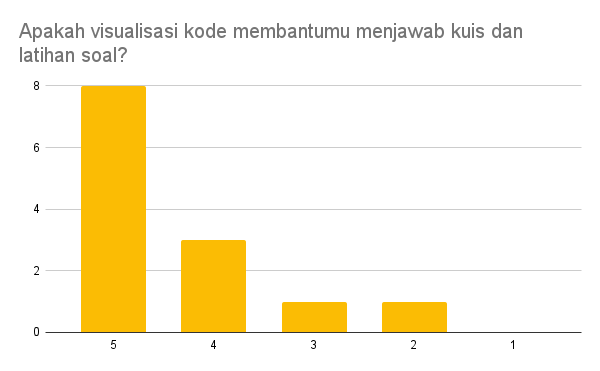
\includegraphics[width=0.7\textwidth]{chapter4/kuesioner-soal.png}
  \caption{Apakah ILE membantu menjawab latihan soal? \\ Sumber: Penulis (2022)} \label{fig:kuesioner-soal}
\end{figure}

\small
\begin{longtable}[c]{|l|>{\setlength{\baselineskip}{0.75\baselineskip}}p{0.5\linewidth}|}
  \caption{Hasil perhitungan statistik deskriptif pada respon kuesioner pertanyaan kedua} \label{tab:kuesioner2-statistik}                                                \\ \hline
                           & Apakah visualisasi kode membantumu menjawab kuis dan latihan soal?                                                                           \\ \hline
  \endfirsthead
  %
  \caption*{\autoref{tab:kuesioner2-statistik} (lanjutan):Hasil perhitungan statistik deskriptif pada respon kuesioner pertanyaan kedua} \label{tab:kuesioner2-statistik} \\ \hline
                           & Apakah visualisasi kode membantumu menjawab kuis dan latihan soal?                                                                           \\ \hline
  \endhead
  %
  Mean                     & 4.384615                                                                                                                                     \\ \hline
  Standard Error           & 0.266469                                                                                                                                     \\ \hline
  Median                   & 5                                                                                                                                            \\ \hline
  Mode                     & 5                                                                                                                                            \\ \hline
  Standard Deviation       & 0.960769                                                                                                                                     \\ \hline
  Sample Variance          & 0.923077                                                                                                                                     \\ \hline
  Kurtosis                 & 2.096086                                                                                                                                     \\ \hline
  Skewness                 & -1.6125                                                                                                                                      \\ \hline
  Range                    & 3                                                                                                                                            \\ \hline
  Minimum                  & 2                                                                                                                                            \\ \hline
  Maximum                  & 5                                                                                                                                            \\ \hline
  Sum                      & 57                                                                                                                                           \\ \hline
  Count                    & 13                                                                                                                                           \\ \hline
  Confidence Level(95,0\%) & 0.580587                                                                                                                                     \\ \hline
\end{longtable}
\normalsize

Berdasarkan \autoref{fig:kuesioner-soal} dan \autoref{tab:kuesioner2-statistik}, dapat disimpulkan bahwa mayoritas peserta eksperimen pada grup perlakuan merasa ILE membantu mereka dalam menjawab kuis serta latihan soal yang diberikan. \textit{Confidence Interval} dengan \textit{Confidence Level} 95\% jatuh pada kisaran nilai 3.804-4.965.

Pada \autoref{fig:kuesioner-average} berikut ditampilkan perbandingan rata-rata respon kuesioner pertanyaan pertama dan kedua.

\begin{figure}[H]
  \centering
  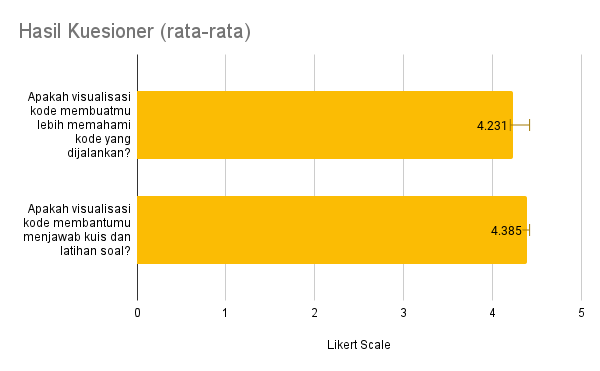
\includegraphics[width=0.9\textwidth]{chapter4/kuesioner-average.png}
  \caption{Perbandingan rata-rata hasil kuesioner ILE \\ Sumber: Penulis (2022)} \label{fig:kuesioner-average}
\end{figure}

Apabila dibandingkan dengan pertanyaan kuesioner pertama, ILE memberikan dampak lebih tinggi dalam membantu memecahkan persoalan. Namun, apabila dilihat dari saran-saran serta pendapat yang diberikan, ILE banyak digunakan untuk memahami proses alur kerja suatu kode. Beberapa peserta pada grup kontrol bahkan memberikan saran untuk memasukkan fitur eksekusi kode pada materi pembelajaran, yang sebenarnya sudah diterapkan pada grup perlakuan. Meskipun dengan jumlah respon yang sedikit, hal ini menjadi indikasi bahwa ILE memiliki dampak dalam pembelajaran pemrograman bagi pemula.

\subsection{Analisis Data Eksperimen}
Setelah dilakukan eksperimen terhadap 25 peserta, didapatkan data penyelesaian modul tiap peserta. Namun, pada hari pertama eksperimen terdapat kesalahan teknis dalam pengambilan data sehingga data beberapa peserta tidak tersimpan. Terdapat 3 peserta pada grup perlakuan yang datanya hilang akibat kesalahan pada basis data, sehingga peserta eksperimen yang dapat diolah datanya berkurang menjadi 22 peserta dengan pembagian 10 peserta grup perlakuan dan 12 peserta grup kontrol. Data lengkap terkait hasil eksperimen dapat dilihat pada

Dari 22 peserta eksperimen, seluruh peserta berhasil menyelesaikan modul pertama (Pengenalan Python Dasar). Namun pada modul kedua (Tipe Data), terdapat 4 peserta (3 peserta grup perlakuan dan 1 peserta grup kontrol) yang tidak berhasil menyelesaikan modul tersebut (tidak berhasil mencapai tahap persoalan) karena keterbatasan waktu eksperimen, sehingga peserta eksperimen yang berhasil menyelesaikan modul kedua berjumlah 18 orang dengan pembagian 7 peserta grup perlakuan dan 11 peserta grup kontrol. Kemudian, peserta yang dapat menyelesaikan modul ketiga (Operator dan Ekspresi) berjumlah 13 orang dengan pembagian 3 peserta grup perlakuan dan 10 peserta grup kontrol. 1 peserta grup kontrol dan 1 peserta grup perlakuan tidak berhasil mencapai tahap persoalan, 2 peserta grup perlakuan hanya mencapai soal kuis kedua (tidak menyelesaikan soal kuis ketiga dan soal latihan kode), dan 1 peserta grup perlakuan hanya mencapai soal kuis ketiga (tidak menyelesaikan soal latihan kode). Karena kurangnya data jumlah peserta eksperimen pada modul 3 serta terdapat perbedaan jumlah peserta grup perlakuan dan grup kontrol yang cukup besar, maka modul yang akan dipakai datanya hanya modul 1 dan modul 2.

Pada analisis data eksperimen ini, akan dilihat juga perbedaan antara data seluruh peserta yang berhasil menyelesaikan suatu modul dengan data peserta yang belum pernah belajar pemrograman sebelumnya dan berhasil menyelesaikan modul tersebut (data peserta setelah penyaringan). Hal ini dilakukan untuk menghilangkan bias dari adanya perbedaan pemahaman awal sehingga menghilangkan beberapa data \textit{outlier}. Pada modul 1, data peserta setelah penyaringan berjumlah 14 orang yaitu 7 peserta grup perlakuan dan 7 peserta grup kontrol. Pada modul 2, data peserta setelah penyaringan berjumlah 11 orang yaitu 6 peserta grup perlakuan dan 5 peserta grup kontrol.


\subsubsection{Analisis Data Eksperimen Soal Kuis}
\begin{figure}[H]
  \centering
  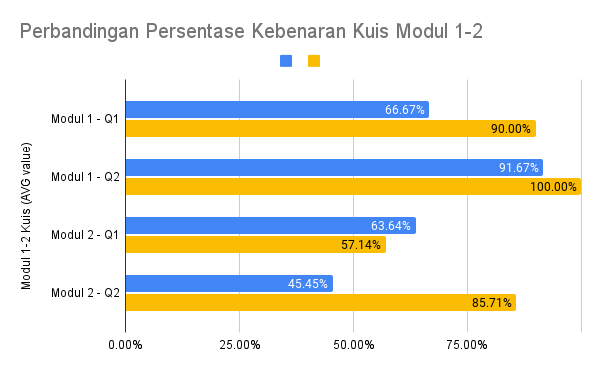
\includegraphics[width=0.85\textwidth]{chapter4/eksperimen-k1k2-kebenaran-all.png}
  \caption{Hasil eksperimen modul 1-2 soal kuis \\ Sumber: Penulis (2022)} \label{fig:eksperimen-k1k2-kebenaran-all}
\end{figure}
\begin{figure}[H]
  \centering
  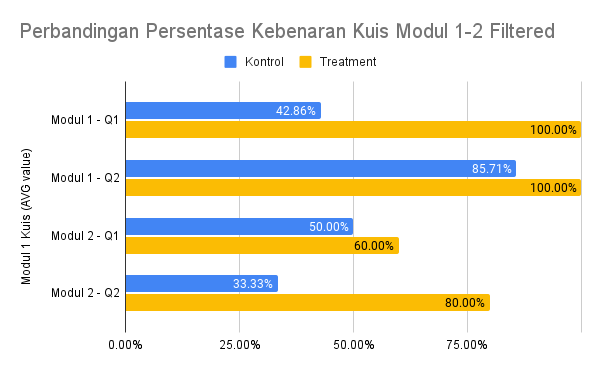
\includegraphics[width=0.85\textwidth]{chapter4/eksperimen-k1k2-kebenaran-awam.png}
  \caption{Hasil eksperimen modul 1-2 soal kuis setelah penyaringan data \\ Sumber: Penulis (2022)} \label{fig:eksperimen-k1k2-kebenaran-awam}
\end{figure}

Berdasarkan pada \autoref{fig:eksperimen-k1k2-kebenaran-all} dan \autoref{fig:eksperimen-k1k2-kebenaran-awam} di atas, dapat dilihat bahwa hasil persentase kuis dengan jawaban yang benar pada grup perlakuan (\textit{treatment}) lebih tinggi rata-ratanya dibandingkan grup kontrol. Terdapat pengecualian pada modul 2 kuis 1 data keseluruhan karena terdapat data \textit{outlier}, tetapi setelah data disaring hasil persentase menjadi lebih konsisten.

Selain dari hasil persentase jawaban, dapat dilihat juga pada \autoref{fig:eksperimen-k1k2-waktu} bahwa waktu pengerjaan kuis grup perlakuan jauh lebih lama dibanding waktu pengerjaan kuis grup kontrol karena peserta melakukan eksplorasi terlebih dahulu pada ILE yang disediakan.

\begin{figure}[H]
  \centering
  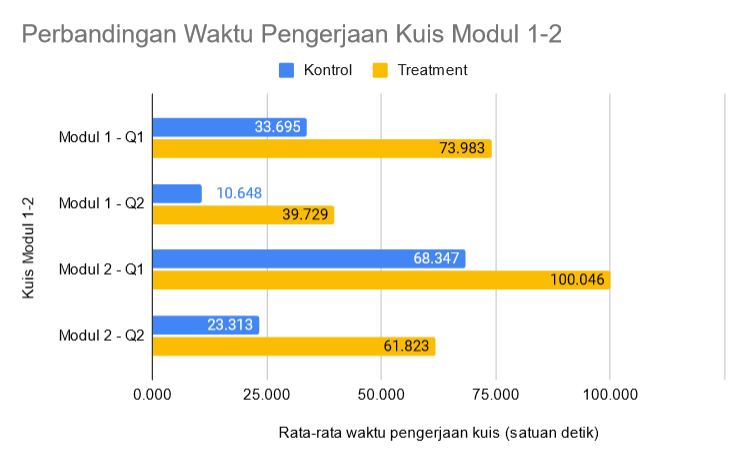
\includegraphics[width=0.85\textwidth]{chapter4/eksperimen-k1k2-waktu.png}
  \caption{Waktu menjawab soal kuis modul 1-2 \\ Sumber: Penulis (2022)} \label{fig:eksperimen-k1k2-waktu}
\end{figure}

\subsubsection{Analisis Data Eksperimen Soal Latihan Kode}
\begin{figure}[H]
  \centering
  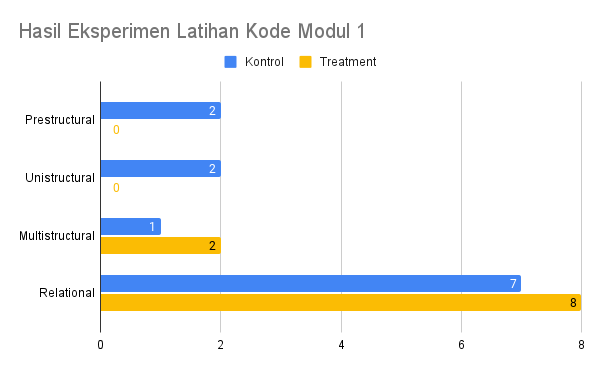
\includegraphics[width=0.85\textwidth]{chapter4/eksperimen-lk1-all.png}
  \caption{Hasil eksperimen modul 1 soal latihan kode \\ Sumber: Penulis (2022)} \label{fig:eksperimen-lk1-all}
\end{figure}
\begin{figure}[H]
  \centering
  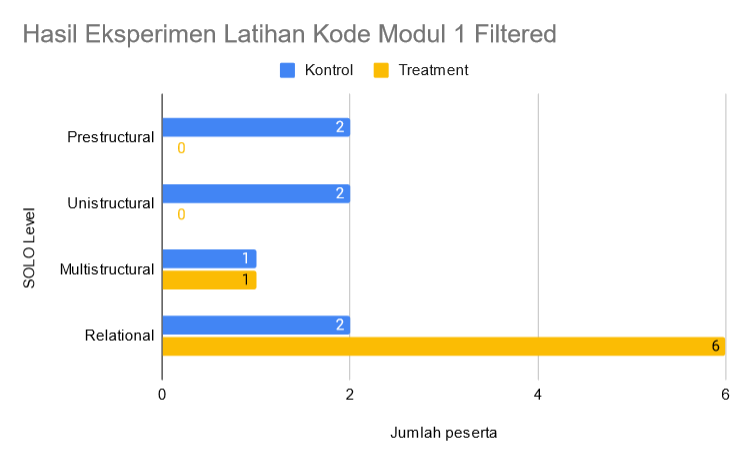
\includegraphics[width=0.85\textwidth]{chapter4/eksperimen-lk1-awam.png}
  \caption{Hasil eksperimen modul 1 soal latihan kode setelah penyaringan data \\ Sumber: Penulis (2022)} \label{fig:eksperimen-lk1-awam}
\end{figure}

Berdasarkan pada \autoref{fig:eksperimen-lk1-all}, dapat dilihat bahwa pada grup perlakuan terdapat lebih banyak peserta yang mendapatkan nilai SOLO Level yang lebih tinggi dengan rata-rata SOLO Level grup perlakuan adalah 3.8 dan rata-rata SOLO Level grup kontrol adalah 3.083. Namun, apabila digunakan \textit{T test} independen dengan asumsi normal distribusi pada data, didapatkan nilai t sebesar 2.086 (\textit{p = 0.097}) yang berarti secara statistik dampak ILE terhadap hasil latihan kode modul 1 tidak terlalu signifikan. Maka dari itu, dilakukan penyaringan data untuk menghilangkan data \textit{outlier} yang dapat mempengaruhi hasil eksperimen. Dapat dilihat pada \autoref{fig:eksperimen-lk1-awam} data yang sudah disaring memiliki perubahan yang cukup besar dengan rata-rata SOLO Level grup perlakuan menjadi 3.857 dan rata-rata SOLO Level grup kontrol menjadi 2.429. Jika dilakukan \textit{T test} pada data yang sudah disaring, didapatkan nilai t sebesar 2.179 (\textit{p = 0.0147}) yang berarti secara statistik dampak ILE terhadap hasil latihan kode modul 1 signifikan.

\begin{figure}[H]
  \centering
  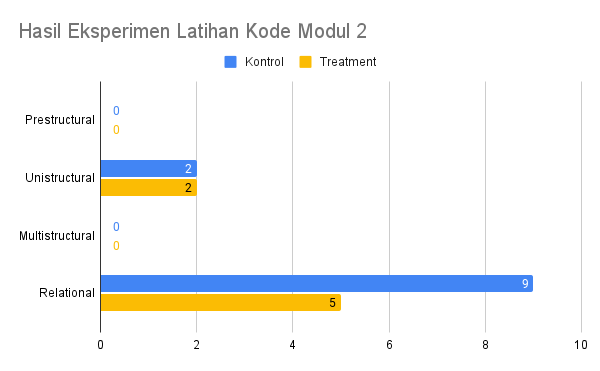
\includegraphics[width=0.85\textwidth]{chapter4/eksperimen-lk2-all.png}
  \caption{Hasil eksperimen modul 2 soal latihan kode \\ Sumber: Penulis (2022)} \label{fig:eksperimen-lk2-all}
\end{figure}
\begin{figure}[H]
  \centering
  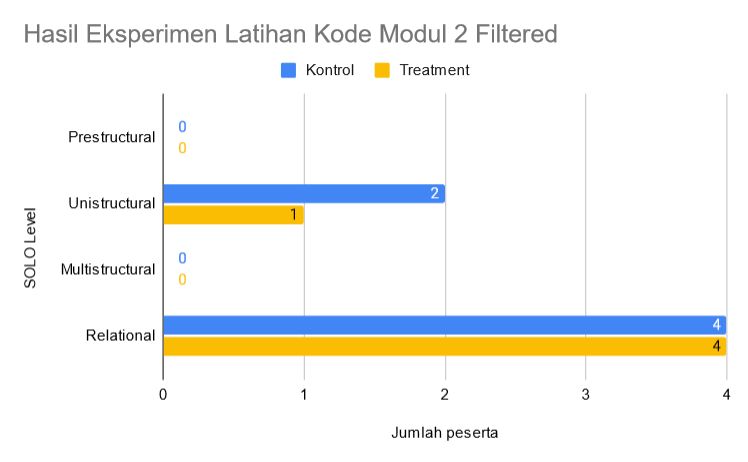
\includegraphics[width=0.85\textwidth]{chapter4/eksperimen-lk2-awam.png}
  \caption{Hasil eksperimen modul 2 soal latihan kode setelah penyaringan data \\ Sumber: Penulis (2022)} \label{fig:eksperimen-lk2-awam}
\end{figure}

Berdasarkan pada \autoref{fig:eksperimen-lk2-all}, rata-rata SOLO Level grup perlakuan adalah 3.429 dan rata-rata SOLO Level grup kontrol adalah 3.636 sehingga grup kontrol memiliki hasil yang lebih tinggi dibanding grup perlakuan. Maka dari itu, dilakukan penyaringan data sehingga data berubah menjadi seperti pada \autoref{fig:eksperimen-lk1-awam}. Data yang sudah disaring memiliki perubahan yang cukup besar dengan rata-rata SOLO Level grup perlakuan menjadi 3.6 dan rata-rata SOLO Level grup kontrol menjadi 3.333 sehingga membuat grup perlakuan memiliki hasil rata-rata yang lebih tinggi dibanding grup kontrol. Namun, jika dilakukan \textit{T test} pada data yang sudah disaring, didapatkan nilai t sebesar 2.262 (\textit{p = 0.662}) yang berarti secara statistik dampak ILE terhadap hasil latihan kode modul 2 tidak signifikan. Salah satu faktor yang menyebabkan hal ini terjadi adalah kurangnya data akibat adanya peserta yang tidak menyelesaikan modul 2 eksperimen. Faktor lain yang dapat berpengaruh pada hasil ini adalah soal yang dibuat kurang bagus sehingga mempengaruhi hasil akhir dari eksperimen.

\subsubsection{Analisis Data Eksperimen Waktu Pengerjaan}
Seperti yang sempat dibahas sebelumnya pada \autoref{fig:eksperimen-k1k2-waktu}, terdapat pola bahwa waktu pengerjaan grup perlakuan jauh lebih lama dibanding grup kontrol. Hal ini dapat dilihat lebih lengkap pada \autoref{fig:eksperimen-m1m2-waktu} yang menampilkan perbandingan rata-rata waktu pengerjaan pada materi, soal kuis, dan soal latihan kode pada modul 1 dan modul 2. Lamanya pengerjaan modul pada grup perlakuan juga menjadi faktor yang membuat grup perlakuan lebih banyak yang tidak menyelesaikan modul 2 dan 3. Setelah diinvestigasi lebih lanjut, ditemukan pada beberapa peserta bahwa ILE dapat menjadi distraksi dalam pembelajaran karena peserta terlalu lama melakukan eksplorasi pada ILE sehingga tidak dapat menyelesaikan modul tepat waktu.

\begin{figure}[H]
  \centering
  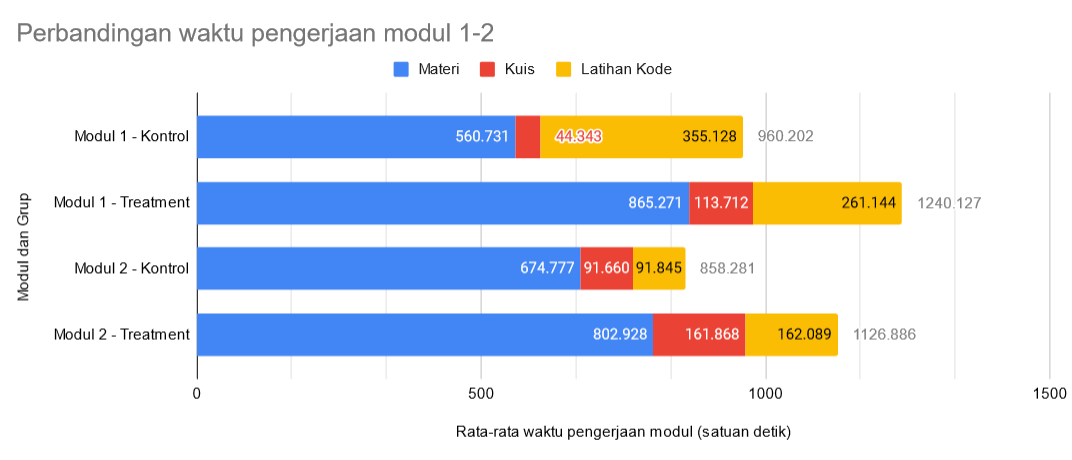
\includegraphics[width=0.85\textwidth]{chapter4/eksperimen-m1m2-waktu.png}
  \caption{Perbandingan waktu pengerjaan modul 1 dan modul 2 \\ Sumber: Penulis (2022)} \label{fig:eksperimen-m1m2-waktu}
\end{figure}

\subsection{Ancaman Validitas (Threat of Validity)}

Pada Laporan Tugas Akhir ini, terdapat beberapa ancaman validitas yang dapat mempengaruhi hasil dari pengujian:
\begin{enumerate}
  \item Pembelajaran hanya dilakukan selama 1 jam sehingga peserta tidak dapat menyelesaikan modul pembelajaran.
  \item Pembelajaran hanya membahas materi dasar agar dapat dipahami dan diselesaikan oleh orang awam. Hal ini membuat pemahaman awal pelajar menjadi krusial karena apabila pelajar telah mempelajari pemrograman sebelumnya, akan timbul data \textit{outlier} yang dapat mempengaruhi hasil eksperimen.
  \item Sulitnya mendapatkan peserta eksperimen dengan pemahaman konsep awal yang sama rata.
  \item Pembuatan materi pembelajaran tidak menggunakan tenaga kerja ahli.
  \item Jumlah sampel yang sedikit dan tidak memenuhi keseluruhan demografis pengguna KodeBareng karena menggunakan teknik \textit{convenience sampling}.
  \item Penilaian jawaban berdasarkan SOLO Level tidak menggunakan tenaga kerja ahli independen.
\end{enumerate}
% \chapter{Kesimpulan dan Saran}

% Bab Kesimpulan dan Saran merupakan penutup dari bagian utama Laporan Tugas Akhir. Fokuskan kesimpulan pada hal-hal baru yang relevan dengan ketercapaian tujuan Tugas Akhir terkait dengan permasalahan yang diselesaikan dalam Tugas Akhir. Saran berisi kajian hal-hal yang masih dapat dikembangkan lebih lanjut.

\section{Kesimpulan}
Setelah dilakukan analisis, implementasi, dan pengujian, dapat diambil kesimpulan sebagai berikut:
\begin{enumerate}
  \item Telah berhasil dikembangkan ILE berupa kakas visualisasi eksekusi kode yang telah diintegrasikan pada platform web pembelajaran pemrograman KodeBareng. ILE tersebut telah diintegrasikan pada modul materi pembelajaran serta soal-soal kuis dan latihan kode sehingga dapat dipakai dan dieksplorasi oleh penggunanya. Saat ini, ILE tersebut masih belum mengimplementasikan keseluruhan fitur yang terdapat pada bahasa pemrograman Python dan masih memiliki keterbatasan dalam visualisasi yang dihasilkan. Keunggulan dari ILE tersebut adalah belum ada platform web pembelajaran pemrograman lain yang memiliki kakas visualisasi eksekusi kode yang terintegrasi pada kelas pembelajarannya sehingga dapat menjadi keunggulan dari platform web pembelajaran pemrograman KodeBareng.
  \item ILE yang telah dibuat memiliki dampak terhadap pengalaman pembelajaran penggunanya, serta memiliki indikasi dapat meningkatkan pemahaman konsep pemrograman dan alur kerja suatu program bagi orang yang belum pernah belajar pemrograman sebelumnya sehingga dapat lebih mudah mempelajari pengenalan dunia pemrograman.
\end{enumerate}

\section{Saran}
Adapun saran terkait pelaksanaan Tugas Akhir ini adalah sebagai berikut:
\begin{enumerate}
  \item Desain tampilan dan interaksi pada komponen visualisasi pada ILE yang telah dikembangkan masih belum mempertimbangkan aspek-aspek psikologis. Dengan mempertimbangkan aspek tersebut, visualisasi yang dibuat akan semakin mudah dimengerti oleh pengguna dan lebih nyaman dalam memakai ILE.
  \item Dukungan terhadap fitur bahasa pemrograman Python yang lebih komprehensif. Penambahan dukungan ini memungkinkan ILE yang dikembangkan dapat digunakan pada kelas pembelajaran yang lebih kompleks.
  \item Konsultasi terhadap tenaga kerja ahli dalam pembuatan materi pembelajaran serta penilaian jawaban sehingga hasil eksperimen yang didapat lebih akurat dan pembelajaran lebih sesuai dengan kaidah-kaidah pendidikan.
\end{enumerate}
%----------------------------------------------------------------%

% Daftar pustaka
\printbibliography
\blankpage

% Setting judul lampiran
\titlespacing*{\chapter}{0pt}{0pt}{0pt}
\titlespacing*{\section}{0pt}{0pt}{*1}

% Setting judul anak lampiran
\titleformat*{\section}{\bfseries}

% Index
\appendix
% \begin{landscape}
  \chapter{Data Eksperimen Modul 1 - Waktu} \label{appendix:data-modul1-waktu}
  \scriptsize
  \begin{longtable}[c]{|l|llllllll|}
    \hline
    \rowcolor[HTML]{C0C0C0}
    \multicolumn{1}{|c|}{\cellcolor[HTML]{C0C0C0}}                                  & \multicolumn{8}{c|}{\cellcolor[HTML]{C0C0C0}\textbf{MODUL 1}}                                                                                                                                                                                                                                                                                                                                                                                                                                                                                                                                                                                         \\ \cline{2-9}
    \rowcolor[HTML]{C0C0C0}
    \multicolumn{1}{|c|}{\cellcolor[HTML]{C0C0C0}}                                  & \multicolumn{4}{c|}{\cellcolor[HTML]{C0C0C0}\textbf{MATERI}}                        & \multicolumn{3}{c|}{\cellcolor[HTML]{C0C0C0}\textbf{SOAL}}                          & \multicolumn{1}{c|}{\cellcolor[HTML]{C0C0C0}}                                                                                                                                                                                                                                                                                                                                                                                                                             \\ \cline{2-8}
    \rowcolor[HTML]{C0C0C0}
    \multicolumn{1}{|c|}{\cellcolor[HTML]{C0C0C0}}                                  & \multicolumn{1}{c|}{\cellcolor[HTML]{C0C0C0}}                                       & \multicolumn{1}{c|}{\cellcolor[HTML]{C0C0C0}}                                       & \multicolumn{1}{c|}{\cellcolor[HTML]{C0C0C0}}                                       & \multicolumn{1}{c|}{\cellcolor[HTML]{C0C0C0}}                                       & \multicolumn{1}{c|}{\cellcolor[HTML]{C0C0C0}\textbf{Quiz \#1}} & \multicolumn{1}{c|}{\cellcolor[HTML]{C0C0C0}\textbf{Quiz \#2}} & \multicolumn{1}{c|}{\cellcolor[HTML]{C0C0C0}\textbf{Latihan Kode}} & \multicolumn{1}{c|}{\cellcolor[HTML]{C0C0C0}}                                          \\ \cline{6-8}
    \rowcolor[HTML]{C0C0C0}
    \multicolumn{1}{|c|}{\multirow{-4}{*}{\cellcolor[HTML]{C0C0C0}\textbf{SUBJEK}}} & \multicolumn{1}{c|}{\multirow{-2}{*}{\cellcolor[HTML]{C0C0C0}\textbf{STAGE 1 (s)}}} & \multicolumn{1}{c|}{\multirow{-2}{*}{\cellcolor[HTML]{C0C0C0}\textbf{STAGE 2 (s)}}} & \multicolumn{1}{c|}{\multirow{-2}{*}{\cellcolor[HTML]{C0C0C0}\textbf{STAGE 3 (s)}}} & \multicolumn{1}{c|}{\multirow{-2}{*}{\cellcolor[HTML]{C0C0C0}\textbf{STAGE 4 (s)}}} & \multicolumn{1}{c|}{\cellcolor[HTML]{C0C0C0}\textbf{time (s)}} & \multicolumn{1}{c|}{\cellcolor[HTML]{C0C0C0}\textbf{time (s)}} & \multicolumn{1}{c|}{\cellcolor[HTML]{C0C0C0}\textbf{time (s)}}     & \multicolumn{1}{c|}{\multirow{-3}{*}{\cellcolor[HTML]{C0C0C0}\textbf{TOTAL TIME (s)}}} \\ \hline
    \endfirsthead
    %
    \multicolumn{9}{c}%
    {{\bfseries Tabel \thetable\ dilanjutkan dari halaman sebelumnya}}                                                                                                                                                                                                                                                                                                                                                                                                                                                                                                                                                                                                                                                                      \\
    \hline
    \rowcolor[HTML]{C0C0C0}
    \multicolumn{1}{|c|}{\cellcolor[HTML]{C0C0C0}}                                  & \multicolumn{8}{c|}{\cellcolor[HTML]{C0C0C0}\textbf{MODUL 1}}                                                                                                                                                                                                                                                                                                                                                                                                                                                                                                                                                                                         \\ \cline{2-9}
    \rowcolor[HTML]{C0C0C0}
    \multicolumn{1}{|c|}{\cellcolor[HTML]{C0C0C0}}                                  & \multicolumn{4}{c|}{\cellcolor[HTML]{C0C0C0}\textbf{MATERI}}                        & \multicolumn{3}{c|}{\cellcolor[HTML]{C0C0C0}\textbf{SOAL}}                          & \multicolumn{1}{c|}{\cellcolor[HTML]{C0C0C0}}                                                                                                                                                                                                                                                                                                                                                                                                                             \\ \cline{2-8}
    \rowcolor[HTML]{C0C0C0}
    \multicolumn{1}{|c|}{\cellcolor[HTML]{C0C0C0}}                                  & \multicolumn{1}{c|}{\cellcolor[HTML]{C0C0C0}}                                       & \multicolumn{1}{c|}{\cellcolor[HTML]{C0C0C0}}                                       & \multicolumn{1}{c|}{\cellcolor[HTML]{C0C0C0}}                                       & \multicolumn{1}{c|}{\cellcolor[HTML]{C0C0C0}}                                       & \multicolumn{1}{c|}{\cellcolor[HTML]{C0C0C0}\textbf{Quiz \#1}} & \multicolumn{1}{c|}{\cellcolor[HTML]{C0C0C0}\textbf{Quiz \#2}} & \multicolumn{1}{c|}{\cellcolor[HTML]{C0C0C0}\textbf{Latihan Kode}} & \multicolumn{1}{c|}{\cellcolor[HTML]{C0C0C0}}                                          \\ \cline{6-8}
    \rowcolor[HTML]{C0C0C0}
    \multicolumn{1}{|c|}{\multirow{-4}{*}{\cellcolor[HTML]{C0C0C0}\textbf{SUBJEK}}} & \multicolumn{1}{c|}{\multirow{-2}{*}{\cellcolor[HTML]{C0C0C0}\textbf{STAGE 1 (s)}}} & \multicolumn{1}{c|}{\multirow{-2}{*}{\cellcolor[HTML]{C0C0C0}\textbf{STAGE 2 (s)}}} & \multicolumn{1}{c|}{\multirow{-2}{*}{\cellcolor[HTML]{C0C0C0}\textbf{STAGE 3 (s)}}} & \multicolumn{1}{c|}{\multirow{-2}{*}{\cellcolor[HTML]{C0C0C0}\textbf{STAGE 4 (s)}}} & \multicolumn{1}{c|}{\cellcolor[HTML]{C0C0C0}\textbf{time (s)}} & \multicolumn{1}{c|}{\cellcolor[HTML]{C0C0C0}\textbf{time (s)}} & \multicolumn{1}{c|}{\cellcolor[HTML]{C0C0C0}\textbf{time (s)}}     & \multicolumn{1}{c|}{\multirow{-3}{*}{\cellcolor[HTML]{C0C0C0}\textbf{TOTAL TIME (s)}}} \\ \hline
    \endhead
    %
    A                                                                               & \multicolumn{1}{l|}{293.415}                                                        & \multicolumn{1}{l|}{316.7}                                                          & \multicolumn{1}{l|}{116.6}                                                          & \multicolumn{1}{l|}{166.7}                                                          & \multicolumn{1}{l|}{44.05}                                     & \multicolumn{1}{l|}{15.314}                                    & \multicolumn{1}{l|}{137.424}                                       & 1090.203                                                                               \\ \hline
    B                                                                               & \multicolumn{1}{l|}{257.398}                                                        & \multicolumn{1}{l|}{604.463}                                                        & \multicolumn{1}{l|}{262.237}                                                        & \multicolumn{1}{l|}{42.5}                                                           & \multicolumn{1}{l|}{32}                                        & \multicolumn{1}{l|}{54.322}                                    & \multicolumn{1}{l|}{40.472}                                        & 1293.392                                                                               \\ \hline
    C                                                                               & \multicolumn{1}{l|}{275.517}                                                        & \multicolumn{1}{l|}{935.04}                                                         & \multicolumn{1}{l|}{222.1}                                                          & \multicolumn{1}{l|}{35.45}                                                          & \multicolumn{1}{l|}{35.45}                                     & \multicolumn{1}{l|}{43.274}                                    & \multicolumn{1}{l|}{47.875}                                        & 1594.706                                                                               \\ \hline
    D                                                                               & \multicolumn{1}{l|}{189.384}                                                        & \multicolumn{1}{l|}{222.293}                                                        & \multicolumn{1}{l|}{220.035}                                                        & \multicolumn{1}{l|}{204.18}                                                         & \multicolumn{1}{l|}{112.389}                                   & \multicolumn{1}{l|}{59.454}                                    & \multicolumn{1}{l|}{72.485}                                        & 1080.221                                                                               \\ \hline
    E                                                                               & \multicolumn{1}{l|}{459.856}                                                        & \multicolumn{1}{l|}{320.287}                                                        & \multicolumn{1}{l|}{259.012}                                                        & \multicolumn{1}{l|}{175.535}                                                        & \multicolumn{1}{l|}{137.503}                                   & \multicolumn{1}{l|}{46.005}                                    & \multicolumn{1}{l|}{154.5}                                         & 1552.698                                                                               \\ \hline
    F                                                                               & \multicolumn{1}{l|}{287.815}                                                        & \multicolumn{1}{l|}{353.454}                                                        & \multicolumn{1}{l|}{125.472}                                                        & \multicolumn{1}{l|}{86.238}                                                         & \multicolumn{1}{l|}{166.923}                                   & \multicolumn{1}{l|}{95.013}                                    & \multicolumn{1}{l|}{791.037}                                       & 1905.952                                                                               \\ \hline
    G                                                                               & \multicolumn{1}{l|}{-}                                                              & \multicolumn{1}{l|}{-}                                                              & \multicolumn{1}{l|}{-}                                                              & \multicolumn{1}{l|}{-}                                                              & \multicolumn{1}{l|}{-}                                         & \multicolumn{1}{l|}{-}                                         & \multicolumn{1}{l|}{-}                                             &                                                                                        \\ \hline
    H                                                                               & \multicolumn{1}{l|}{-}                                                              & \multicolumn{1}{l|}{-}                                                              & \multicolumn{1}{l|}{-}                                                              & \multicolumn{1}{l|}{-}                                                              & \multicolumn{1}{l|}{-}                                         & \multicolumn{1}{l|}{-}                                         & \multicolumn{1}{l|}{-}                                             &                                                                                        \\ \hline
    I                                                                               & \multicolumn{1}{l|}{218.273}                                                        & \multicolumn{1}{l|}{235}                                                            & \multicolumn{1}{l|}{298.587}                                                        & \multicolumn{1}{l|}{144.79}                                                         & \multicolumn{1}{l|}{148.478}                                   & \multicolumn{1}{l|}{28.842}                                    & \multicolumn{1}{l|}{769.834}                                       & 1843.804                                                                               \\ \hline
    J                                                                               & \multicolumn{1}{l|}{-}                                                              & \multicolumn{1}{l|}{-}                                                              & \multicolumn{1}{l|}{-}                                                              & \multicolumn{1}{l|}{-}                                                              & \multicolumn{1}{l|}{-}                                         & \multicolumn{1}{l|}{-}                                         & \multicolumn{1}{l|}{-}                                             &                                                                                        \\ \hline
    K                                                                               & \multicolumn{1}{l|}{20.398}                                                         & \multicolumn{1}{l|}{33.742}                                                         & \multicolumn{1}{l|}{11.742}                                                         & \multicolumn{1}{l|}{10.399}                                                         & \multicolumn{1}{l|}{28.479}                                    & \multicolumn{1}{l|}{15.521}                                    & \multicolumn{1}{l|}{524.095}                                       & 644.376                                                                                \\ \hline
    L                                                                               & \multicolumn{1}{l|}{316.698}                                                        & \multicolumn{1}{l|}{341.1}                                                          & \multicolumn{1}{l|}{144.01}                                                         & \multicolumn{1}{l|}{42.76}                                                          & \multicolumn{1}{l|}{12.85}                                     & \multicolumn{1}{l|}{12.8}                                      & \multicolumn{1}{l|}{40.02}                                         & 910.238                                                                                \\ \hline
    M                                                                               & \multicolumn{1}{l|}{29.448}                                                         & \multicolumn{1}{l|}{248.62}                                                         & \multicolumn{1}{l|}{107.33}                                                         & \multicolumn{1}{l|}{18.13}                                                          & \multicolumn{1}{l|}{21.71}                                     & \multicolumn{1}{l|}{26.74}                                     & \multicolumn{1}{l|}{33.7}                                          & 485.678                                                                                \\ \hline
    N                                                                               & \multicolumn{1}{l|}{77.1}                                                           & \multicolumn{1}{l|}{312.965}                                                        & \multicolumn{1}{l|}{165.18}                                                         & \multicolumn{1}{l|}{94.523}                                                         & \multicolumn{1}{l|}{11.435}                                    & \multicolumn{1}{l|}{9.318}                                     & \multicolumn{1}{l|}{54.077}                                        & 724.598                                                                                \\ \hline
    O                                                                               & \multicolumn{1}{l|}{47.693}                                                         & \multicolumn{1}{l|}{164.429}                                                        & \multicolumn{1}{l|}{99.364}                                                         & \multicolumn{1}{l|}{29.15}                                                          & \multicolumn{1}{l|}{9.535}                                     & \multicolumn{1}{l|}{9.67}                                      & \multicolumn{1}{l|}{26.429}                                        & 386.27                                                                                 \\ \hline
    P                                                                               & \multicolumn{1}{l|}{55.558}                                                         & \multicolumn{1}{l|}{271.001}                                                        & \multicolumn{1}{l|}{296.664}                                                        & \multicolumn{1}{l|}{123.31}                                                         & \multicolumn{1}{l|}{15.779}                                    & \multicolumn{1}{l|}{6.098}                                     & \multicolumn{1}{l|}{267.083}                                       & 1035.493                                                                               \\ \hline
    Q                                                                               & \multicolumn{1}{l|}{132.544}                                                        & \multicolumn{1}{l|}{156.229}                                                        & \multicolumn{1}{l|}{186.068}                                                        & \multicolumn{1}{l|}{43.1}                                                           & \multicolumn{1}{l|}{5.692}                                     & \multicolumn{1}{l|}{9.669}                                     & \multicolumn{1}{l|}{27.494}                                        & 560.796                                                                                \\ \hline
    R                                                                               & \multicolumn{1}{l|}{122.306}                                                        & \multicolumn{1}{l|}{170.504}                                                        & \multicolumn{1}{l|}{145.725}                                                        & \multicolumn{1}{l|}{38.396}                                                         & \multicolumn{1}{l|}{18.057}                                    & \multicolumn{1}{l|}{9.9}                                       & \multicolumn{1}{l|}{26.196}                                        & 531.084                                                                                \\ \hline
    S                                                                               & \multicolumn{1}{l|}{51.833}                                                         & \multicolumn{1}{l|}{324.777}                                                        & \multicolumn{1}{l|}{253.079}                                                        & \multicolumn{1}{l|}{108.927}                                                        & \multicolumn{1}{l|}{231.6}                                     & \multicolumn{1}{l|}{14.413}                                    & \multicolumn{1}{l|}{1771.583}                                      & 2756.212                                                                               \\ \hline
    T                                                                               & \multicolumn{1}{l|}{193.47}                                                         & \multicolumn{1}{l|}{72.446}                                                         & \multicolumn{1}{l|}{144.525}                                                        & \multicolumn{1}{l|}{72.072}                                                         & \multicolumn{1}{l|}{13.552}                                    & \multicolumn{1}{l|}{12.38}                                     & \multicolumn{1}{l|}{48.823}                                        & 557.268                                                                                \\ \hline
    U                                                                               & \multicolumn{1}{l|}{54.129}                                                         & \multicolumn{1}{l|}{77.156}                                                         & \multicolumn{1}{l|}{100.171}                                                        & \multicolumn{1}{l|}{12.861}                                                         & \multicolumn{1}{l|}{10.038}                                    & \multicolumn{1}{l|}{15.305}                                    & \multicolumn{1}{l|}{26.592}                                        & 296.252                                                                                \\ \hline
    V                                                                               & \multicolumn{1}{l|}{41.49}                                                          & \multicolumn{1}{l|}{239.918}                                                        & \multicolumn{1}{l|}{204.475}                                                        & \multicolumn{1}{l|}{101.685}                                                        & \multicolumn{1}{l|}{15.793}                                    & \multicolumn{1}{l|}{6.503}                                     & \multicolumn{1}{l|}{289.636}                                       & 899.5                                                                                  \\ \hline
    W                                                                               & \multicolumn{1}{l|}{92.121}                                                         & \multicolumn{1}{l|}{273.24}                                                         & \multicolumn{1}{l|}{448.259}                                                        & \multicolumn{1}{l|}{53.164}                                                         & \multicolumn{1}{l|}{22.449}                                    & \multicolumn{1}{l|}{10.322}                                    & \multicolumn{1}{l|}{109.901}                                       & 1009.456                                                                               \\ \hline
    X                                                                               & \multicolumn{1}{l|}{106.011}                                                        & \multicolumn{1}{l|}{246.341}                                                        & \multicolumn{1}{l|}{197.729}                                                        & \multicolumn{1}{l|}{50.648}                                                         & \multicolumn{1}{l|}{17.522}                                    & \multicolumn{1}{l|}{16.274}                                    & \multicolumn{1}{l|}{1499.625}                                      & 2134.15                                                                                \\ \hline
    Y                                                                               & \multicolumn{1}{l|}{154.695}                                                        & \multicolumn{1}{l|}{150.705}                                                        & \multicolumn{1}{l|}{128.683}                                                        & \multicolumn{1}{l|}{42.349}                                                         & \multicolumn{1}{l|}{32.89}                                     & \multicolumn{1}{l|}{7.921}                                     & \multicolumn{1}{l|}{114.1}                                         & 631.343                                                                                \\ \hline
  \end{longtable}
\end{landscape}

\begin{landscape}
  \chapter{Data Eksperimen Modul 1 - Jawaban} \label{appendix:data-modul1-jawaban}
  \tiny
  \begin{longtable}[c]{|l|lllllllll>{\raggedright\arraybackslash\setlength{\baselineskip}{0.75\baselineskip}}p{0.1\linewidth}|}
    \hline
    \rowcolor[HTML]{C0C0C0}
    \multicolumn{1}{|c|}{\cellcolor[HTML]{C0C0C0}}                                  & \multicolumn{10}{c|}{\cellcolor[HTML]{C0C0C0}\textbf{MODUL 1}}                                                                                                                                                                                                                                                                                                                                                                                                                                                                                                                                                                                                                                                                                                                                                                                                                                                                                                                                                                                                                                                                                                                                                                                                                                                                                                                                                                                                                                                                                                                                                                                                                                                                                                                                                                                                                                                                                                                                                                                                                                                                                                                              \\ \cline{2-11}
    \rowcolor[HTML]{C0C0C0}
    \multicolumn{1}{|c|}{\cellcolor[HTML]{C0C0C0}}                                  & \multicolumn{9}{c|}{\cellcolor[HTML]{C0C0C0}\textbf{SOAL}}        & \multicolumn{1}{c|}{\cellcolor[HTML]{C0C0C0}}                                                                                                                                                                                                                                                                                                                                                                                                                                                                                                                                                                                                                                                                                                                                                                                                                                                                                                                                                                                                                                                                                                                                                                                                                                                                                                                                                                                                                                                                                                                                                                                                                                                                                                                                                                                                                                                                                                                                                                                                                                                                    \\ \cline{2-10}
    \rowcolor[HTML]{C0C0C0}
    \multicolumn{1}{|c|}{\cellcolor[HTML]{C0C0C0}}                                  & \multicolumn{3}{c|}{\cellcolor[HTML]{C0C0C0}\textbf{Quiz \#1}}    & \multicolumn{3}{c|}{\cellcolor[HTML]{C0C0C0}\textbf{Quiz \#2}}  & \multicolumn{3}{c|}{\cellcolor[HTML]{C0C0C0}\textbf{Latihan Kode}}                                                                                                                                                                                                                                            & \multicolumn{1}{c|}{\cellcolor[HTML]{C0C0C0}}                                                                                                                                                                                                                                                                                                                                                                                                                                                                                                                                                                                                                                                                                                                                                                                                                                                                                                                                                                                                                                                                                                                                                                                                                                                                                                                                                                                                                                                                                                                                                                                                                                                                                  \\ \cline{2-10}
    \rowcolor[HTML]{C0C0C0}
    \multicolumn{1}{|c|}{\multirow{-4}{*}{\cellcolor[HTML]{C0C0C0}\textbf{SUBJEK}}} & \multicolumn{1}{c|}{\cellcolor[HTML]{C0C0C0}\textbf{value (1/0)}} & \multicolumn{1}{c|}{\cellcolor[HTML]{C0C0C0}\textbf{retry (n)}} & \multicolumn{1}{c|}{\cellcolor[HTML]{C0C0C0}\textbf{answers (str)}}                                                                                                                                                                                                                                           & \multicolumn{1}{c|}{\cellcolor[HTML]{C0C0C0}\textbf{value (1/0)}} & \multicolumn{1}{c|}{\cellcolor[HTML]{C0C0C0}\textbf{retry (n)}} & \multicolumn{1}{c|}{\cellcolor[HTML]{C0C0C0}\textbf{answers (str)}} & \multicolumn{1}{c|}{\cellcolor[HTML]{C0C0C0}\textbf{value(n/4)}} & \multicolumn{1}{c|}{\cellcolor[HTML]{C0C0C0}\textbf{retry (n)}} & \multicolumn{1}{c|}{\cellcolor[HTML]{C0C0C0}\textbf{answers (str)}}                                                                                                                                                                                                                                                                                                                                                                                                                                                                                                                                                                                                                                                                                                                                                                                                                                                                                                                                                                                                                                                                                                                                                                                                                           & \multicolumn{1}{c|}{\multirow{-3}{*}{\cellcolor[HTML]{C0C0C0}\textbf{NOTES}}} \\ \hline
    \endfirsthead
    %
    \multicolumn{11}{c}%
    {{\bfseries Tabel \thetable\ dilanjutkan dari halaman sebelumnya}}                                                                                                                                                                                                                                                                                                                                                                                                                                                                                                                                                                                                                                                                                                                                                                                                                                                                                                                                                                                                                                                                                                                                                                                                                                                                                                                                                                                                                                                                                                                                                                                                                                                                                                                                                                                                                                                                                                                                                                                                                                                                                                                                                                                                     \\
    \hline
    \rowcolor[HTML]{C0C0C0}
    \multicolumn{1}{|c|}{\cellcolor[HTML]{C0C0C0}}                                  & \multicolumn{10}{c|}{\cellcolor[HTML]{C0C0C0}\textbf{MODUL 1}}                                                                                                                                                                                                                                                                                                                                                                                                                                                                                                                                                                                                                                                                                                                                                                                                                                                                                                                                                                                                                                                                                                                                                                                                                                                                                                                                                                                                                                                                                                                                                                                                                                                                                                                                                                                                                                                                                                                                                                                                                                                                                                                              \\ \cline{2-11}
    \rowcolor[HTML]{C0C0C0}
    \multicolumn{1}{|c|}{\cellcolor[HTML]{C0C0C0}}                                  & \multicolumn{9}{c|}{\cellcolor[HTML]{C0C0C0}\textbf{SOAL}}        & \multicolumn{1}{c|}{\cellcolor[HTML]{C0C0C0}}                                                                                                                                                                                                                                                                                                                                                                                                                                                                                                                                                                                                                                                                                                                                                                                                                                                                                                                                                                                                                                                                                                                                                                                                                                                                                                                                                                                                                                                                                                                                                                                                                                                                                                                                                                                                                                                                                                                                                                                                                                                                    \\ \cline{2-10}
    \rowcolor[HTML]{C0C0C0}
    \multicolumn{1}{|c|}{\cellcolor[HTML]{C0C0C0}}                                  & \multicolumn{3}{c|}{\cellcolor[HTML]{C0C0C0}\textbf{Quiz \#1}}    & \multicolumn{3}{c|}{\cellcolor[HTML]{C0C0C0}\textbf{Quiz \#2}}  & \multicolumn{3}{c|}{\cellcolor[HTML]{C0C0C0}\textbf{Latihan Kode}}                                                                                                                                                                                                                                            & \multicolumn{1}{c|}{\cellcolor[HTML]{C0C0C0}}                                                                                                                                                                                                                                                                                                                                                                                                                                                                                                                                                                                                                                                                                                                                                                                                                                                                                                                                                                                                                                                                                                                                                                                                                                                                                                                                                                                                                                                                                                                                                                                                                                                                                  \\ \cline{2-10}
    \rowcolor[HTML]{C0C0C0}
    \multicolumn{1}{|c|}{\multirow{-4}{*}{\cellcolor[HTML]{C0C0C0}\textbf{SUBJEK}}} & \multicolumn{1}{c|}{\cellcolor[HTML]{C0C0C0}\textbf{value (1/0)}} & \multicolumn{1}{c|}{\cellcolor[HTML]{C0C0C0}\textbf{retry (n)}} & \multicolumn{1}{c|}{\cellcolor[HTML]{C0C0C0}\textbf{answers (str)}}                                                                                                                                                                                                                                           & \multicolumn{1}{c|}{\cellcolor[HTML]{C0C0C0}\textbf{value (1/0)}} & \multicolumn{1}{c|}{\cellcolor[HTML]{C0C0C0}\textbf{retry (n)}} & \multicolumn{1}{c|}{\cellcolor[HTML]{C0C0C0}\textbf{answers (str)}} & \multicolumn{1}{c|}{\cellcolor[HTML]{C0C0C0}\textbf{value(n/4)}} & \multicolumn{1}{c|}{\cellcolor[HTML]{C0C0C0}\textbf{retry (n)}} & \multicolumn{1}{c|}{\cellcolor[HTML]{C0C0C0}\textbf{answers (str)}}                                                                                                                                                                                                                                                                                                                                                                                                                                                                                                                                                                                                                                                                                                                                                                                                                                                                                                                                                                                                                                                                                                                                                                                                                           & \multicolumn{1}{c|}{\multirow{-3}{*}{\cellcolor[HTML]{C0C0C0}\textbf{NOTES}}} \\ \hline
    \endhead
    %
    A                                                                               & \multicolumn{1}{l|}{1}                                            & \multicolumn{1}{l|}{0}                                          & \multicolumn{1}{>{\raggedright\arraybackslash\setlength{\baselineskip}{0.75\baselineskip}}p{0.1\linewidth}|}{Menampilkan sesuatu pada program}                                                                                                                                                                & \multicolumn{1}{l|}{1}                                            & \multicolumn{1}{l|}{0}                                          & \multicolumn{1}{l|}{3}                                              & \multicolumn{1}{l|}{4}                                           & \multicolumn{1}{l|}{1}                                          & \multicolumn{1}{>{\raggedright\arraybackslash\setlength{\baselineskip}{0.75\baselineskip}}p{0.2\linewidth}|}{\begin{tabular}[c]{@{}>{\raggedright\arraybackslash\setlength{\baselineskip}{0.75\baselineskip}}p{\linewidth}@{}}print(\textbackslash{}"Hello World\textbackslash{}")\\ print(\textbackslash{}"Halo Dunia!\textbackslash{}")\end{tabular}}                                                                                                                                                                                                                                                                                                                                                                                                                                                                                                                                                                                                                                                                                                                                                                                                                                                                                                                                       &                                                                               \\ \hline
    B                                                                               & \multicolumn{1}{l|}{1}                                            & \multicolumn{1}{l|}{0}                                          & \multicolumn{1}{>{\raggedright\arraybackslash\setlength{\baselineskip}{0.75\baselineskip}}p{0.1\linewidth}|}{Menampilkan sesuatu pada program}                                                                                                                                                                & \multicolumn{1}{l|}{1}                                            & \multicolumn{1}{l|}{0}                                          & \multicolumn{1}{l|}{3}                                              & \multicolumn{1}{l|}{4}                                           & \multicolumn{1}{l|}{0}                                          & \multicolumn{1}{>{\raggedright\arraybackslash\setlength{\baselineskip}{0.75\baselineskip}}p{0.2\linewidth}|}{print(\textbackslash{}"Halo Dunia!\textbackslash{}")}                                                                                                                                                                                                                                                                                                                                                                                                                                                                                                                                                                                                                                                                                                                                                                                                                                                                                                                                                                                                                                                                                                                            &                                                                               \\ \hline
    C                                                                               & \multicolumn{1}{l|}{1}                                            & \multicolumn{1}{l|}{0}                                          & \multicolumn{1}{>{\raggedright\arraybackslash\setlength{\baselineskip}{0.75\baselineskip}}p{0.1\linewidth}|}{Menampilkan sesuatu pada program}                                                                                                                                                                & \multicolumn{1}{l|}{1}                                            & \multicolumn{1}{l|}{0}                                          & \multicolumn{1}{l|}{3}                                              & \multicolumn{1}{l|}{4}                                           & \multicolumn{1}{l|}{0}                                          & \multicolumn{1}{>{\raggedright\arraybackslash\setlength{\baselineskip}{0.75\baselineskip}}p{0.2\linewidth}|}{print(\textbackslash{}"Halo Dunia!\textbackslash{}")}                                                                                                                                                                                                                                                                                                                                                                                                                                                                                                                                                                                                                                                                                                                                                                                                                                                                                                                                                                                                                                                                                                                            & Pernah belajar \textless 6 bulan tapi masih awam                              \\ \hline
    D                                                                               & \multicolumn{1}{l|}{1}                                            & \multicolumn{1}{l|}{0}                                          & \multicolumn{1}{>{\raggedright\arraybackslash\setlength{\baselineskip}{0.75\baselineskip}}p{0.1\linewidth}|}{Menampilkan sesuatu pada program}                                                                                                                                                                & \multicolumn{1}{l|}{1}                                            & \multicolumn{1}{l|}{0}                                          & \multicolumn{1}{l|}{3}                                              & \multicolumn{1}{l|}{3}                                           & \multicolumn{1}{l|}{2}                                          & \multicolumn{1}{>{\raggedright\arraybackslash\setlength{\baselineskip}{0.75\baselineskip}}p{0.2\linewidth}|}{\begin{tabular}[c]{@{}>{\raggedright\arraybackslash\setlength{\baselineskip}{0.75\baselineskip}}p{\linewidth}@{}}x = input (\textbackslash{}"Halo DUnia\textbackslash{}"\textbackslash{}r\textbackslash{}nx = x + \textbackslash{}"!\textbackslash{}"\textbackslash{}r\textbackslash{}nprint(x)\\ x = input(\textbackslash{}"Halo Dunia\textbackslash{}")\textbackslash{}r\textbackslash{}nX = X + \textbackslash{}"!\textbackslash{}" \textbackslash{}r\textbackslash{}nprint(\textbackslash{}"Halo Dunia\textbackslash{}")\\ print(\textbackslash{}"Halo Dunia!\textbackslash{}")\end{tabular}}                                                                                                                                                                                                                                                                                                                                                                                                                                                                                                                                                                                &                                                                               \\ \hline
    E                                                                               & \multicolumn{1}{l|}{1}                                            & \multicolumn{1}{l|}{0}                                          & \multicolumn{1}{>{\raggedright\arraybackslash\setlength{\baselineskip}{0.75\baselineskip}}p{0.1\linewidth}|}{Menampilkan sesuatu pada program}                                                                                                                                                                & \multicolumn{1}{l|}{1}                                            & \multicolumn{1}{l|}{0}                                          & \multicolumn{1}{l|}{3}                                              & \multicolumn{1}{l|}{4}                                           & \multicolumn{1}{l|}{2}                                          & \multicolumn{1}{>{\raggedright\arraybackslash\setlength{\baselineskip}{0.75\baselineskip}}p{0.2\linewidth}|}{\begin{tabular}[c]{@{}>{\raggedright\arraybackslash\setlength{\baselineskip}{0.75\baselineskip}}p{\linewidth}@{}}print(\textbackslash{}"Hello World\textbackslash{}")\\ print(\textbackslash{}"Halo Dunia\textbackslash{}")\\ print(\textbackslash{}"Halo Dunia!\textbackslash{}")\end{tabular}}                                                                                                                                                                                                                                                                                                                                                                                                                                                                                                                                                                                                                                                                                                                                                                                                                                                                                 &                                                                               \\ \hline
    F                                                                               & \multicolumn{1}{l|}{1}                                            & \multicolumn{1}{l|}{0}                                          & \multicolumn{1}{>{\raggedright\arraybackslash\setlength{\baselineskip}{0.75\baselineskip}}p{0.1\linewidth}|}{Menampilkan sesuatu pada program}                                                                                                                                                                & \multicolumn{1}{l|}{1}                                            & \multicolumn{1}{l|}{0}                                          & \multicolumn{1}{l|}{3}                                              & \multicolumn{1}{l|}{4}                                           & \multicolumn{1}{l|}{3}                                          & \multicolumn{1}{>{\raggedright\arraybackslash\setlength{\baselineskip}{0.75\baselineskip}}p{0.2\linewidth}|}{\begin{tabular}[c]{@{}>{\raggedright\arraybackslash\setlength{\baselineskip}{0.75\baselineskip}}p{\linewidth}@{}}\# print(\textbackslash{}"Hello World\textbackslash{}")\\ print(\textbackslash{}"Hello World\textbackslash{}")\\ print(\textbackslash{}"Halo Dunia\textbackslash{}"\\ print(\textbackslash{}"Halo Dunia!\textbackslash{}")\end{tabular}}                                                                                                                                                                                                                                                                                                                                                                                                                                                                                                                                                                                                                                                                                                                                                                                                                        &                                                                               \\ \hline
    G                                                                               & \multicolumn{1}{l|}{-}                                            & \multicolumn{1}{l|}{-}                                          & \multicolumn{1}{>{\raggedright\arraybackslash\setlength{\baselineskip}{0.75\baselineskip}}p{0.1\linewidth}|}{-}                                                                                                                                                                                               & \multicolumn{1}{l|}{-}                                            & \multicolumn{1}{l|}{-}                                          & \multicolumn{1}{l|}{-}                                              & \multicolumn{1}{l|}{-}                                           & \multicolumn{1}{l|}{-}                                          & \multicolumn{1}{>{\raggedright\arraybackslash\setlength{\baselineskip}{0.75\baselineskip}}p{0.2\linewidth}|}{-}                                                                                                                                                                                                                                                                                                                                                                                                                                                                                                                                                                                                                                                                                                                                                                                                                                                                                                                                                                                                                                                                                                                                                                               &                                                                               \\ \hline
    H                                                                               & \multicolumn{1}{l|}{-}                                            & \multicolumn{1}{l|}{-}                                          & \multicolumn{1}{>{\raggedright\arraybackslash\setlength{\baselineskip}{0.75\baselineskip}}p{0.1\linewidth}|}{-}                                                                                                                                                                                               & \multicolumn{1}{l|}{-}                                            & \multicolumn{1}{l|}{-}                                          & \multicolumn{1}{l|}{-}                                              & \multicolumn{1}{l|}{-}                                           & \multicolumn{1}{l|}{-}                                          & \multicolumn{1}{>{\raggedright\arraybackslash\setlength{\baselineskip}{0.75\baselineskip}}p{0.2\linewidth}|}{-}                                                                                                                                                                                                                                                                                                                                                                                                                                                                                                                                                                                                                                                                                                                                                                                                                                                                                                                                                                                                                                                                                                                                                                               &                                                                               \\ \hline
    I                                                                               & \multicolumn{1}{l|}{1}                                            & \multicolumn{1}{l|}{0}                                          & \multicolumn{1}{>{\raggedright\arraybackslash\setlength{\baselineskip}{0.75\baselineskip}}p{0.1\linewidth}|}{Menampilkan sesuatu pada program}                                                                                                                                                                & \multicolumn{1}{l|}{1}                                            & \multicolumn{1}{l|}{0}                                          & \multicolumn{1}{l|}{3}                                              & \multicolumn{1}{l|}{4}                                           & \multicolumn{1}{l|}{4}                                          & \multicolumn{1}{>{\raggedright\arraybackslash\setlength{\baselineskip}{0.75\baselineskip}}p{0.2\linewidth}|}{\begin{tabular}[c]{@{}>{\raggedright\arraybackslash\setlength{\baselineskip}{0.75\baselineskip}}p{\linewidth}@{}}print(Hello World)\\ print(\textbackslash{}"Hello World\textbackslash{}")\\ x = input ()\textbackslash{}r\textbackslash{}nprint (x)\\ input (\textbackslash{}"Hello World\textbackslash{}")\textbackslash{}r\textbackslash{}nprint (\textbackslash{}"Halo Dunia!\textbackslash{}")\\ print(\textbackslash{}"Halo Dunia!\textbackslash{}")\end{tabular}}                                                                                                                                                                                                                                                                                                                                                                                                                                                                                                                                                                                                                                                                                                         &                                                                               \\ \hline
    J                                                                               & \multicolumn{1}{l|}{-}                                            & \multicolumn{1}{l|}{-}                                          & \multicolumn{1}{>{\raggedright\arraybackslash\setlength{\baselineskip}{0.75\baselineskip}}p{0.1\linewidth}|}{-}                                                                                                                                                                                               & \multicolumn{1}{l|}{-}                                            & \multicolumn{1}{l|}{-}                                          & \multicolumn{1}{l|}{-}                                              & \multicolumn{1}{l|}{-}                                           & \multicolumn{1}{l|}{-}                                          & \multicolumn{1}{>{\raggedright\arraybackslash\setlength{\baselineskip}{0.75\baselineskip}}p{0.2\linewidth}|}{-}                                                                                                                                                                                                                                                                                                                                                                                                                                                                                                                                                                                                                                                                                                                                                                                                                                                                                                                                                                                                                                                                                                                                                                               &                                                                               \\ \hline
    K                                                                               & \multicolumn{1}{l|}{1}                                            & \multicolumn{1}{l|}{0}                                          & \multicolumn{1}{>{\raggedright\arraybackslash\setlength{\baselineskip}{0.75\baselineskip}}p{0.1\linewidth}|}{Menampilkan sesuatu pada program}                                                                                                                                                                & \multicolumn{1}{l|}{1}                                            & \multicolumn{1}{l|}{0}                                          & \multicolumn{1}{l|}{3}                                              & \multicolumn{1}{l|}{3}                                           & \multicolumn{1}{l|}{11}                                         & \multicolumn{1}{>{\raggedright\arraybackslash\setlength{\baselineskip}{0.75\baselineskip}}p{0.2\linewidth}|}{\begin{tabular}[c]{@{}>{\raggedright\arraybackslash\setlength{\baselineskip}{0.75\baselineskip}}p{\linewidth}@{}}print(\textbackslash{}"halo dunia!\textbackslash{}")\\ print(\textbackslash{}"halo dunia\textbackslash{}"!)\\ print(\textbackslash{}"halo dunia!\textbackslash{}")\\ print(\textbackslash{}"halodunia!\textbackslash{}")\\ print(\textbackslash{}"Halo dunia!\textbackslash{}")\\ \#print(\textbackslash{}"Halo dunia!\textbackslash{}")\\ \# print(\textbackslash{}"Halo dunia!\textbackslash{}")\\ \# print(\textbackslash{}"Halo dunia!\textbackslash{}")\\ \# print(\textbackslash{}"Halo dunia!\textbackslash{}")\\  print(\textbackslash{}"Hallo dunia!\textbackslash{}")\\  print(\textbackslash{}"Halo Dunia!\textbackslash{}")\\ print(\textbackslash{}"Halo Dunia!\textbackslash{}")\end{tabular}}                                                                                                                                                                                                                                                                                                                                                    & Pernah belajar \textless 6 bulan                                              \\ \hline
    L                                                                               & \multicolumn{1}{l|}{1}                                            & \multicolumn{1}{l|}{0}                                          & \multicolumn{1}{>{\raggedright\arraybackslash\setlength{\baselineskip}{0.75\baselineskip}}p{0.1\linewidth}|}{Menampilkan sesuatu pada program}                                                                                                                                                                & \multicolumn{1}{l|}{1}                                            & \multicolumn{1}{l|}{0}                                          & \multicolumn{1}{l|}{3}                                              & \multicolumn{1}{l|}{4}                                           & \multicolumn{1}{l|}{0}                                          & \multicolumn{1}{>{\raggedright\arraybackslash\setlength{\baselineskip}{0.75\baselineskip}}p{0.2\linewidth}|}{print(\textbackslash{}"Halo Dunia!\textbackslash{}")}                                                                                                                                                                                                                                                                                                                                                                                                                                                                                                                                                                                                                                                                                                                                                                                                                                                                                                                                                                                                                                                                                                                            &                                                                               \\ \hline
    M                                                                               & \multicolumn{1}{l|}{0}                                            & \multicolumn{1}{l|}{1}                                          & \multicolumn{1}{>{\raggedright\arraybackslash\setlength{\baselineskip}{0.75\baselineskip}}p{0.1\linewidth}|}{\begin{tabular}[c]{@{}>{\raggedright\arraybackslash\setlength{\baselineskip}{0.75\baselineskip}}p{\linewidth}@{}}Meminta masukkan dari pengguna\\ Menampilkan sesuatu pada program\end{tabular}} & \multicolumn{1}{l|}{1}                                            & \multicolumn{1}{l|}{0}                                          & \multicolumn{1}{l|}{3}                                              & \multicolumn{1}{l|}{4}                                           & \multicolumn{1}{l|}{1}                                          & \multicolumn{1}{>{\raggedright\arraybackslash\setlength{\baselineskip}{0.75\baselineskip}}p{0.2\linewidth}|}{\begin{tabular}[c]{@{}>{\raggedright\arraybackslash\setlength{\baselineskip}{0.75\baselineskip}}p{\linewidth}@{}}print(\textbackslash{}"Hello World\textbackslash{}")\\ print(\textbackslash{}"Halo Dunia!\textbackslash{}")\end{tabular}}                                                                                                                                                                                                                                                                                                                                                                                                                                                                                                                                                                                                                                                                                                                                                                                                                                                                                                                                       & Pernah belajar 6-12 bulan, udah mayan jago                                    \\ \hline
    N                                                                               & \multicolumn{1}{l|}{1}                                            & \multicolumn{1}{l|}{0}                                          & \multicolumn{1}{>{\raggedright\arraybackslash\setlength{\baselineskip}{0.75\baselineskip}}p{0.1\linewidth}|}{Menampilkan sesuatu pada program}                                                                                                                                                                & \multicolumn{1}{l|}{1}                                            & \multicolumn{1}{l|}{0}                                          & \multicolumn{1}{l|}{3}                                              & \multicolumn{1}{l|}{4}                                           & \multicolumn{1}{l|}{0}                                          & \multicolumn{1}{>{\raggedright\arraybackslash\setlength{\baselineskip}{0.75\baselineskip}}p{0.2\linewidth}|}{print (\textbackslash{}"Halo Dunia!\textbackslash{}")}                                                                                                                                                                                                                                                                                                                                                                                                                                                                                                                                                                                                                                                                                                                                                                                                                                                                                                                                                                                                                                                                                                                           &                                                                               \\ \hline
    O                                                                               & \multicolumn{1}{l|}{1}                                            & \multicolumn{1}{l|}{0}                                          & \multicolumn{1}{>{\raggedright\arraybackslash\setlength{\baselineskip}{0.75\baselineskip}}p{0.1\linewidth}|}{Menampilkan sesuatu pada program}                                                                                                                                                                & \multicolumn{1}{l|}{1}                                            & \multicolumn{1}{l|}{0}                                          & \multicolumn{1}{l|}{3}                                              & \multicolumn{1}{l|}{4}                                           & \multicolumn{1}{l|}{0}                                          & \multicolumn{1}{>{\raggedright\arraybackslash\setlength{\baselineskip}{0.75\baselineskip}}p{0.2\linewidth}|}{print(\textbackslash{}"Halo Dunia!\textbackslash{}")}                                                                                                                                                                                                                                                                                                                                                                                                                                                                                                                                                                                                                                                                                                                                                                                                                                                                                                                                                                                                                                                                                                                            & Pernah belajar 6-12 bulan, udah jago                                          \\ \hline
    P                                                                               & \multicolumn{1}{l|}{1}                                            & \multicolumn{1}{l|}{0}                                          & \multicolumn{1}{>{\raggedright\arraybackslash\setlength{\baselineskip}{0.75\baselineskip}}p{0.1\linewidth}|}{Menampilkan sesuatu pada program}                                                                                                                                                                & \multicolumn{1}{l|}{1}                                            & \multicolumn{1}{l|}{0}                                          & \multicolumn{1}{l|}{3}                                              & \multicolumn{1}{l|}{2}                                           & \multicolumn{1}{l|}{7}                                          & \multicolumn{1}{>{\raggedright\arraybackslash\setlength{\baselineskip}{0.75\baselineskip}}p{0.2\linewidth}|}{\begin{tabular}[c]{@{}>{\raggedright\arraybackslash\setlength{\baselineskip}{0.75\baselineskip}}p{\linewidth}@{}}print (\textbackslash{}"hello world\textbackslash{}")\\ print (\textbackslash{}"Hello World\textbackslash{}")\\ x = (\textbackslash{}"Hello World\textbackslash{}")\textbackslash{}r\textbackslash{}nprint (x)\\ x = int (input (\textbackslash{}"Hello World\textbackslash{}"))\textbackslash{}r\textbackslash{}nprint(\textbackslash{}"x\textbackslash{}")\\ print(\textbackslash{}"Hello World\textbackslash{}")\\ print('hello world')\\ print('Halo Dunia')\\ print('Halo Dunia!')\end{tabular}}                                                                                                                                                                                                                                                                                                                                                                                                                                                                                                                                                           & Pakai VSCode                                                                  \\ \hline
    Q                                                                               & \multicolumn{1}{l|}{1}                                            & \multicolumn{1}{l|}{0}                                          & \multicolumn{1}{>{\raggedright\arraybackslash\setlength{\baselineskip}{0.75\baselineskip}}p{0.1\linewidth}|}{Menampilkan sesuatu pada program}                                                                                                                                                                & \multicolumn{1}{l|}{1}                                            & \multicolumn{1}{l|}{0}                                          & \multicolumn{1}{l|}{3}                                              & \multicolumn{1}{l|}{4}                                           & \multicolumn{1}{l|}{0}                                          & \multicolumn{1}{>{\raggedright\arraybackslash\setlength{\baselineskip}{0.75\baselineskip}}p{0.2\linewidth}|}{print(\textbackslash{}"Halo Dunia!\textbackslash{}")}                                                                                                                                                                                                                                                                                                                                                                                                                                                                                                                                                                                                                                                                                                                                                                                                                                                                                                                                                                                                                                                                                                                            & Pernah belajar \textless 6 bulan                                              \\ \hline
    R                                                                               & \multicolumn{1}{l|}{1}                                            & \multicolumn{1}{l|}{0}                                          & \multicolumn{1}{>{\raggedright\arraybackslash\setlength{\baselineskip}{0.75\baselineskip}}p{0.1\linewidth}|}{Menampilkan sesuatu pada program}                                                                                                                                                                & \multicolumn{1}{l|}{1}                                            & \multicolumn{1}{l|}{0}                                          & \multicolumn{1}{l|}{3}                                              & \multicolumn{1}{l|}{4}                                           & \multicolumn{1}{l|}{0}                                          & \multicolumn{1}{>{\raggedright\arraybackslash\setlength{\baselineskip}{0.75\baselineskip}}p{0.2\linewidth}|}{print(\textbackslash{}"Halo Dunia!\textbackslash{}")}                                                                                                                                                                                                                                                                                                                                                                                                                                                                                                                                                                                                                                                                                                                                                                                                                                                                                                                                                                                                                                                                                                                            & Pernah belajar \textless 6 bulan, udah jago                                   \\ \hline
    S                                                                               & \multicolumn{1}{l|}{0}                                            & \multicolumn{1}{l|}{1}                                          & \multicolumn{1}{>{\raggedright\arraybackslash\setlength{\baselineskip}{0.75\baselineskip}}p{0.1\linewidth}|}{\begin{tabular}[c]{@{}>{\raggedright\arraybackslash\setlength{\baselineskip}{0.75\baselineskip}}p{\linewidth}@{}}Meminta masukkan dari pengguna\\ Menampilkan sesuatu pada program\end{tabular}} & \multicolumn{1}{l|}{1}                                            & \multicolumn{1}{l|}{0}                                          & \multicolumn{1}{l|}{3}                                              & \multicolumn{1}{l|}{1}                                           & \multicolumn{1}{l|}{3}                                          & \multicolumn{1}{>{\raggedright\arraybackslash\setlength{\baselineskip}{0.75\baselineskip}}p{0.2\linewidth}|}{\begin{tabular}[c]{@{}>{\raggedright\arraybackslash\setlength{\baselineskip}{0.75\baselineskip}}p{\linewidth}@{}}A = int(input()\textbackslash{}r\textbackslash{}nB = int(input())\textbackslash{}r\textbackslash{}nA = A + B\textbackslash{}r\textbackslash{}nprint(A)\\ A = int(input()\textbackslash{}r\textbackslash{}nB = int(input())\textbackslash{}r\textbackslash{}nA = A + B\textbackslash{}r\textbackslash{}nprint(A)\\ A = int(input())\textbackslash{}r\textbackslash{}nB = int(input())\textbackslash{}r\textbackslash{}nA = A + B\textbackslash{}r\textbackslash{}nprint(A)\\ print(\textbackslash{}"Halo Dunia!\textbackslash{}")\end{tabular}}                                                                                                                                                                                                                                                                                                                                                                                                                                                                                                                  &                                                                               \\ \hline
    T                                                                               & \multicolumn{1}{l|}{1}                                            & \multicolumn{1}{l|}{0}                                          & \multicolumn{1}{>{\raggedright\arraybackslash\setlength{\baselineskip}{0.75\baselineskip}}p{0.1\linewidth}|}{Menampilkan sesuatu pada program}                                                                                                                                                                & \multicolumn{1}{l|}{1}                                            & \multicolumn{1}{l|}{0}                                          & \multicolumn{1}{l|}{3}                                              & \multicolumn{1}{l|}{4}                                           & \multicolumn{1}{l|}{0}                                          & \multicolumn{1}{>{\raggedright\arraybackslash\setlength{\baselineskip}{0.75\baselineskip}}p{0.2\linewidth}|}{print(\textbackslash{}"Halo Dunia!\textbackslash{}")}                                                                                                                                                                                                                                                                                                                                                                                                                                                                                                                                                                                                                                                                                                                                                                                                                                                                                                                                                                                                                                                                                                                            & Pernah belajar \textless 6 bulan, mayan jago                                  \\ \hline
    U                                                                               & \multicolumn{1}{l|}{1}                                            & \multicolumn{1}{l|}{0}                                          & \multicolumn{1}{>{\raggedright\arraybackslash\setlength{\baselineskip}{0.75\baselineskip}}p{0.1\linewidth}|}{Menampilkan sesuatu pada program}                                                                                                                                                                & \multicolumn{1}{l|}{1}                                            & \multicolumn{1}{l|}{0}                                          & \multicolumn{1}{l|}{3}                                              & \multicolumn{1}{l|}{4}                                           & \multicolumn{1}{l|}{0}                                          & \multicolumn{1}{>{\raggedright\arraybackslash\setlength{\baselineskip}{0.75\baselineskip}}p{0.2\linewidth}|}{print(\textbackslash{}"Halo Dunia!\textbackslash{}")}                                                                                                                                                                                                                                                                                                                                                                                                                                                                                                                                                                                                                                                                                                                                                                                                                                                                                                                                                                                                                                                                                                                            & Pernah belajar \textless 6 bulan, mayan jago                                  \\ \hline
    V                                                                               & \multicolumn{1}{l|}{0}                                            & \multicolumn{1}{l|}{1}                                          & \multicolumn{1}{>{\raggedright\arraybackslash\setlength{\baselineskip}{0.75\baselineskip}}p{0.1\linewidth}|}{\begin{tabular}[c]{@{}>{\raggedright\arraybackslash\setlength{\baselineskip}{0.75\baselineskip}}p{\linewidth}@{}}Tidak dieksekusi oleh komputer\\ Menampilkan sesuatu pada program\end{tabular}} & \multicolumn{1}{l|}{1}                                            & \multicolumn{1}{l|}{0}                                          & \multicolumn{1}{l|}{3}                                              & \multicolumn{1}{l|}{2}                                           & \multicolumn{1}{l|}{1}                                          & \multicolumn{1}{>{\raggedright\arraybackslash\setlength{\baselineskip}{0.75\baselineskip}}p{0.2\linewidth}|}{\begin{tabular}[c]{@{}>{\raggedright\arraybackslash\setlength{\baselineskip}{0.75\baselineskip}}p{\linewidth}@{}}x = input(\textbackslash{}"Hello Word\textbackslash{}")\textbackslash{}r\textbackslash{}nx = x + \textbackslash{}"!\textbackslash{}"\textbackslash{}r\textbackslash{}nprint(x)\\ print(\textbackslash{}"Halo Dunia!\textbackslash{}")\end{tabular}}                                                                                                                                                                                                                                                                                                                                                                                                                                                                                                                                                                                                                                                                                                                                                                                                             &                                                                               \\ \hline
    W                                                                               & \multicolumn{1}{l|}{0}                                            & \multicolumn{1}{l|}{1}                                          & \multicolumn{1}{>{\raggedright\arraybackslash\setlength{\baselineskip}{0.75\baselineskip}}p{0.1\linewidth}|}{\begin{tabular}[c]{@{}>{\raggedright\arraybackslash\setlength{\baselineskip}{0.75\baselineskip}}p{\linewidth}@{}}Menjumlahkan 2 angka\\ Menampilkan sesuatu pada program\end{tabular}}           & \multicolumn{1}{l|}{1}                                            & \multicolumn{1}{l|}{0}                                          & \multicolumn{1}{l|}{3}                                              & \multicolumn{1}{l|}{3}                                           & \multicolumn{1}{l|}{4}                                          & \multicolumn{1}{>{\raggedright\arraybackslash\setlength{\baselineskip}{0.75\baselineskip}}p{0.2\linewidth}|}{\begin{tabular}[c]{@{}>{\raggedright\arraybackslash\setlength{\baselineskip}{0.75\baselineskip}}p{\linewidth}@{}}print(\textbackslash{}"halo dunia\textbackslash{}")+!\\ print(\textbackslash{}"halo dunia!\textbackslash{}")\\ print(halo dunia!)\\ print(\textbackslash{}"halo dunia!\textbackslash{}")\\ print(\textbackslash{}"Halo Dunia!\textbackslash{}")\end{tabular}}                                                                                                                                                                                                                                                                                                                                                                                                                                                                                                                                                                                                                                                                                                                                                                                                   &                                                                               \\ \hline
    X                                                                               & \multicolumn{1}{l|}{0}                                            & \multicolumn{1}{l|}{1}                                          & \multicolumn{1}{>{\raggedright\arraybackslash\setlength{\baselineskip}{0.75\baselineskip}}p{0.1\linewidth}|}{\begin{tabular}[c]{@{}>{\raggedright\arraybackslash\setlength{\baselineskip}{0.75\baselineskip}}p{\linewidth}@{}}Menjumlahkan 2 angka\\ Menampilkan sesuatu pada program\end{tabular}}           & \multicolumn{1}{l|}{0}                                            & \multicolumn{1}{l|}{1}                                          & \multicolumn{1}{l|}{\begin{tabular}[c]{@{}l@{}}2\\ 3\end{tabular}}  & \multicolumn{1}{l|}{1}                                           & \multicolumn{1}{l|}{10}                                         & \multicolumn{1}{>{\raggedright\arraybackslash\setlength{\baselineskip}{0.75\baselineskip}}p{0.2\linewidth}|}{\begin{tabular}[c]{@{}>{\raggedright\arraybackslash\setlength{\baselineskip}{0.75\baselineskip}}p{\linewidth}@{}}\textbackslash{}"Hello World!\textbackslash{}"\\ \textbackslash{}"Hallo Dunia!\textbackslash{}"\\ x= Hello World\textbackslash{}nx= \textbackslash{}"Hello World!\textbackslash{}"\textbackslash{}nprint(x)\\ x= Hello World\textbackslash{}nx= \textbackslash{}"Hello World!\textbackslash{}"\textbackslash{}nprint\\ Hello World\textbackslash{}n\textbackslash{}"Hello World!\textbackslash{}"\textbackslash{}nprint(\textbackslash{}"Hello World!\textbackslash{}")\\ Hello World\textbackslash{}n\textbackslash{}"Hello World!\textbackslash{}"\textbackslash{}nprint(Halo Dunia!)\\ Hello World\textbackslash{}n\textbackslash{}"Hello World!\textbackslash{}nHalo Dunia!\\ Halo Dunia\textbackslash{}n\textbackslash{}"Halo Dunia!\textbackslash{}"\textbackslash{}n\#print(\textbackslash{}"Halo Dunia\textbackslash{}")\\ Halo Dunia\textbackslash{}n\textbackslash{}"Halo Dunia!\textbackslash{}"\textbackslash{}n\#print\\ print(\textbackslash{}"Hello World\textbackslash{}")\\ print(\textbackslash{}"Halo Dunia!\textbackslash{}")\end{tabular}} &                                                                               \\ \hline
    Y                                                                               & \multicolumn{1}{l|}{1}                                            & \multicolumn{1}{l|}{0}                                          & \multicolumn{1}{>{\raggedright\arraybackslash\setlength{\baselineskip}{0.75\baselineskip}}p{0.1\linewidth}|}{Menampilkan sesuatu pada program}                                                                                                                                                                & \multicolumn{1}{l|}{1}                                            & \multicolumn{1}{l|}{0}                                          & \multicolumn{1}{l|}{3}                                              & \multicolumn{1}{l|}{4}                                           & \multicolumn{1}{l|}{1}                                          & \multicolumn{1}{>{\raggedright\arraybackslash\setlength{\baselineskip}{0.75\baselineskip}}p{0.2\linewidth}|}{\begin{tabular}[c]{@{}>{\raggedright\arraybackslash\setlength{\baselineskip}{0.75\baselineskip}}p{\linewidth}@{}}print(\textbackslash{}"Hello World!\textbackslash{}")\\ print(\textbackslash{}"Halo Dunia!\textbackslash{}")\end{tabular}}                                                                                                                                                                                                                                                                                                                                                                                                                                                                                                                                                                                                                                                                                                                                                                                                                                                                                                                                      & Udah jago, pernah belajar C\# di SMA                                          \\ \hline
  \end{longtable}
\end{landscape}
% \begin{landscape}
\chapter{Data Eksperimen Modul 2 - Waktu} \label{appendix:data-modul2-waktu}
\scriptsize
  \begin{longtable}[c]{|l|llllllllll|}
  \hline
  \rowcolor[HTML]{C0C0C0} 
  \multicolumn{1}{|c|}{\cellcolor[HTML]{C0C0C0}}                                  & \multicolumn{10}{c|}{\cellcolor[HTML]{C0C0C0}\textbf{MODUL 2}}                                                                                                                                                                                                                                                                                                                                                                                                                                                                                                                                                                                                                                                                                                                                                                    \\ \cline{2-11} 
  \rowcolor[HTML]{C0C0C0} 
  \multicolumn{1}{|c|}{\cellcolor[HTML]{C0C0C0}}                                  & \multicolumn{6}{c|}{\cellcolor[HTML]{C0C0C0}\textbf{MATERI}}                                                                                                                                                                                                                                                                                                                                                                                                                                                                      & \multicolumn{3}{c|}{\cellcolor[HTML]{C0C0C0}\textbf{SOAL}}                                                                                                                                           & \multicolumn{1}{c|}{\cellcolor[HTML]{C0C0C0}}                                          \\ \cline{2-10}
  \rowcolor[HTML]{C0C0C0} 
  \multicolumn{1}{|c|}{\cellcolor[HTML]{C0C0C0}}                                  & \multicolumn{1}{c|}{\cellcolor[HTML]{C0C0C0}}                                       & \multicolumn{1}{c|}{\cellcolor[HTML]{C0C0C0}}                                       & \multicolumn{1}{c|}{\cellcolor[HTML]{C0C0C0}}                                       & \multicolumn{1}{c|}{\cellcolor[HTML]{C0C0C0}}                                       & \multicolumn{1}{c|}{\cellcolor[HTML]{C0C0C0}}                                       & \multicolumn{1}{c|}{\cellcolor[HTML]{C0C0C0}}                                       & \multicolumn{1}{c|}{\cellcolor[HTML]{C0C0C0}\textbf{Quiz \#1}} & \multicolumn{1}{c|}{\cellcolor[HTML]{C0C0C0}\textbf{Quiz \#2}} & \multicolumn{1}{c|}{\cellcolor[HTML]{C0C0C0}\textbf{Latihan Kode}} & \multicolumn{1}{c|}{\cellcolor[HTML]{C0C0C0}}                                          \\ \cline{8-10}
  \rowcolor[HTML]{C0C0C0} 
  \multicolumn{1}{|c|}{\multirow{-4}{*}{\cellcolor[HTML]{C0C0C0}\textbf{SUBJEK}}} & \multicolumn{1}{c|}{\multirow{-2}{*}{\cellcolor[HTML]{C0C0C0}\textbf{STAGE 1 (s)}}} & \multicolumn{1}{c|}{\multirow{-2}{*}{\cellcolor[HTML]{C0C0C0}\textbf{STAGE 2 (s)}}} & \multicolumn{1}{c|}{\multirow{-2}{*}{\cellcolor[HTML]{C0C0C0}\textbf{STAGE 3 (s)}}} & \multicolumn{1}{c|}{\multirow{-2}{*}{\cellcolor[HTML]{C0C0C0}\textbf{STAGE 4 (s)}}} & \multicolumn{1}{c|}{\multirow{-2}{*}{\cellcolor[HTML]{C0C0C0}\textbf{STAGE 5 (s)}}} & \multicolumn{1}{c|}{\multirow{-2}{*}{\cellcolor[HTML]{C0C0C0}\textbf{STAGE 6 (s)}}} & \multicolumn{1}{c|}{\cellcolor[HTML]{C0C0C0}\textbf{time (s)}} & \multicolumn{1}{c|}{\cellcolor[HTML]{C0C0C0}\textbf{time (s)}} & \multicolumn{1}{c|}{\cellcolor[HTML]{C0C0C0}\textbf{time (s)}}     & \multicolumn{1}{c|}{\multirow{-3}{*}{\cellcolor[HTML]{C0C0C0}\textbf{TOTAL TIME (s)}}} \\ \hline
  \endfirsthead
  %
  \multicolumn{11}{c}%
  {{\bfseries Tabel \thetable\ dilanjutkan dari halaman sebelumnya}} \\
  \hline
  \rowcolor[HTML]{C0C0C0} 
  \multicolumn{1}{|c|}{\cellcolor[HTML]{C0C0C0}}                                  & \multicolumn{10}{c|}{\cellcolor[HTML]{C0C0C0}\textbf{MODUL 2}}                                                                                                                                                                                                                                                                                                                                                                                                                                                                                                                                                                                                                                                                                                                                                                    \\ \cline{2-11} 
  \rowcolor[HTML]{C0C0C0} 
  \multicolumn{1}{|c|}{\cellcolor[HTML]{C0C0C0}}                                  & \multicolumn{6}{c|}{\cellcolor[HTML]{C0C0C0}\textbf{MATERI}}                                                                                                                                                                                                                                                                                                                                                                                                                                                                      & \multicolumn{3}{c|}{\cellcolor[HTML]{C0C0C0}\textbf{SOAL}}                                                                                                                                           & \multicolumn{1}{c|}{\cellcolor[HTML]{C0C0C0}}                                          \\ \cline{2-10}
  \rowcolor[HTML]{C0C0C0} 
  \multicolumn{1}{|c|}{\cellcolor[HTML]{C0C0C0}}                                  & \multicolumn{1}{c|}{\cellcolor[HTML]{C0C0C0}}                                       & \multicolumn{1}{c|}{\cellcolor[HTML]{C0C0C0}}                                       & \multicolumn{1}{c|}{\cellcolor[HTML]{C0C0C0}}                                       & \multicolumn{1}{c|}{\cellcolor[HTML]{C0C0C0}}                                       & \multicolumn{1}{c|}{\cellcolor[HTML]{C0C0C0}}                                       & \multicolumn{1}{c|}{\cellcolor[HTML]{C0C0C0}}                                       & \multicolumn{1}{c|}{\cellcolor[HTML]{C0C0C0}\textbf{Quiz \#1}} & \multicolumn{1}{c|}{\cellcolor[HTML]{C0C0C0}\textbf{Quiz \#2}} & \multicolumn{1}{c|}{\cellcolor[HTML]{C0C0C0}\textbf{Latihan Kode}} & \multicolumn{1}{c|}{\cellcolor[HTML]{C0C0C0}}                                          \\ \cline{8-10}
  \rowcolor[HTML]{C0C0C0} 
  \multicolumn{1}{|c|}{\multirow{-4}{*}{\cellcolor[HTML]{C0C0C0}\textbf{SUBJEK}}} & \multicolumn{1}{c|}{\multirow{-2}{*}{\cellcolor[HTML]{C0C0C0}\textbf{STAGE 1 (s)}}} & \multicolumn{1}{c|}{\multirow{-2}{*}{\cellcolor[HTML]{C0C0C0}\textbf{STAGE 2 (s)}}} & \multicolumn{1}{c|}{\multirow{-2}{*}{\cellcolor[HTML]{C0C0C0}\textbf{STAGE 3 (s)}}} & \multicolumn{1}{c|}{\multirow{-2}{*}{\cellcolor[HTML]{C0C0C0}\textbf{STAGE 4 (s)}}} & \multicolumn{1}{c|}{\multirow{-2}{*}{\cellcolor[HTML]{C0C0C0}\textbf{STAGE 5 (s)}}} & \multicolumn{1}{c|}{\multirow{-2}{*}{\cellcolor[HTML]{C0C0C0}\textbf{STAGE 6 (s)}}} & \multicolumn{1}{c|}{\cellcolor[HTML]{C0C0C0}\textbf{time (s)}} & \multicolumn{1}{c|}{\cellcolor[HTML]{C0C0C0}\textbf{time (s)}} & \multicolumn{1}{c|}{\cellcolor[HTML]{C0C0C0}\textbf{time (s)}}     & \multicolumn{1}{c|}{\multirow{-3}{*}{\cellcolor[HTML]{C0C0C0}\textbf{TOTAL TIME (s)}}} \\ \hline
  \endhead
  %
  A                                                                               & \multicolumn{1}{l|}{141.7}                                                          & \multicolumn{1}{l|}{154.195}                                                        & \multicolumn{1}{l|}{69.163}                                                         & \multicolumn{1}{l|}{61.314}                                                         & \multicolumn{1}{l|}{146.591}                                                        & \multicolumn{1}{l|}{387.264}                                                        & \multicolumn{1}{l|}{-}                                         & \multicolumn{1}{l|}{-}                                         & \multicolumn{1}{l|}{-}                                             & 960.227                                                                                \\ \hline
  B                                                                               & \multicolumn{1}{l|}{58.3}                                                           & \multicolumn{1}{l|}{133.9}                                                          & \multicolumn{1}{l|}{153.6}                                                          & \multicolumn{1}{l|}{111.9}                                                          & \multicolumn{1}{l|}{293}                                                            & \multicolumn{1}{l|}{470.253}                                                        & \multicolumn{1}{l|}{-}                                         & \multicolumn{1}{l|}{-}                                         & \multicolumn{1}{l|}{-}                                             & 1220.953                                                                               \\ \hline
  C                                                                               & \multicolumn{1}{l|}{216.8}                                                          & \multicolumn{1}{l|}{73}                                                             & \multicolumn{1}{l|}{235}                                                            & \multicolumn{1}{l|}{294}                                                            & \multicolumn{1}{l|}{300}                                                            & \multicolumn{1}{l|}{106.491}                                                        & \multicolumn{1}{l|}{-}                                         & \multicolumn{1}{l|}{-}                                         & \multicolumn{1}{l|}{-}                                             & 1225.291                                                                               \\ \hline
  D                                                                               & \multicolumn{1}{l|}{213.7}                                                          & \multicolumn{1}{l|}{131.065}                                                        & \multicolumn{1}{l|}{143.599}                                                        & \multicolumn{1}{l|}{91.645}                                                         & \multicolumn{1}{l|}{46.595}                                                         & \multicolumn{1}{l|}{331.413}                                                        & \multicolumn{1}{l|}{165.585}                                   & \multicolumn{1}{l|}{165.585}                                   & \multicolumn{1}{l|}{165.585}                                       & 1454.772                                                                               \\ \hline
  E                                                                               & \multicolumn{1}{l|}{392.177}                                                        & \multicolumn{1}{l|}{110.27}                                                         & \multicolumn{1}{l|}{102.286}                                                        & \multicolumn{1}{l|}{103.2}                                                          & \multicolumn{1}{l|}{18.817}                                                         & \multicolumn{1}{l|}{263.648}                                                        & \multicolumn{1}{l|}{271.935}                                   & \multicolumn{1}{l|}{53.595}                                    & \multicolumn{1}{l|}{325.53}                                        & 1641.458                                                                               \\ \hline
  F                                                                               & \multicolumn{1}{l|}{210.291}                                                        & \multicolumn{1}{l|}{72.371}                                                         & \multicolumn{1}{l|}{46.469}                                                         & \multicolumn{1}{l|}{112.5}                                                          & \multicolumn{1}{l|}{115.2}                                                          & \multicolumn{1}{l|}{270.968}                                                        & \multicolumn{1}{l|}{77.855}                                    & \multicolumn{1}{l|}{117.354}                                   & \multicolumn{1}{l|}{194.571}                                       & 1217.579                                                                               \\ \hline
  G                                                                               & \multicolumn{1}{l|}{-}                                                              & \multicolumn{1}{l|}{-}                                                              & \multicolumn{1}{l|}{-}                                                              & \multicolumn{1}{l|}{-}                                                              & \multicolumn{1}{l|}{-}                                                              & \multicolumn{1}{l|}{-}                                                              & \multicolumn{1}{l|}{-}                                         & \multicolumn{1}{l|}{-}                                         & \multicolumn{1}{l|}{-}                                             &                                                                                        \\ \hline
  H                                                                               & \multicolumn{1}{l|}{-}                                                              & \multicolumn{1}{l|}{-}                                                              & \multicolumn{1}{l|}{-}                                                              & \multicolumn{1}{l|}{-}                                                              & \multicolumn{1}{l|}{-}                                                              & \multicolumn{1}{l|}{-}                                                              & \multicolumn{1}{l|}{-}                                         & \multicolumn{1}{l|}{-}                                         & \multicolumn{1}{l|}{-}                                             &                                                                                        \\ \hline
  I                                                                               & \multicolumn{1}{l|}{147.11}                                                         & \multicolumn{1}{l|}{74.361}                                                         & \multicolumn{1}{l|}{36.379}                                                         & \multicolumn{1}{l|}{45.249}                                                         & \multicolumn{1}{l|}{36.331}                                                         & \multicolumn{1}{l|}{173.093}                                                        & \multicolumn{1}{l|}{70.131}                                    & \multicolumn{1}{l|}{44.203}                                    & \multicolumn{1}{l|}{195.895}                                       & 822.752                                                                                \\ \hline
  J                                                                               & \multicolumn{1}{l|}{-}                                                              & \multicolumn{1}{l|}{-}                                                              & \multicolumn{1}{l|}{-}                                                              & \multicolumn{1}{l|}{-}                                                              & \multicolumn{1}{l|}{-}                                                              & \multicolumn{1}{l|}{-}                                                              & \multicolumn{1}{l|}{-}                                         & \multicolumn{1}{l|}{-}                                         & \multicolumn{1}{l|}{-}                                             &                                                                                        \\ \hline
  K                                                                               & \multicolumn{1}{l|}{18.359}                                                         & \multicolumn{1}{l|}{10.277}                                                         & \multicolumn{1}{l|}{11.824}                                                         & \multicolumn{1}{l|}{10.444}                                                         & \multicolumn{1}{l|}{9.227}                                                          & \multicolumn{1}{l|}{17.772}                                                         & \multicolumn{1}{l|}{47.754}                                    & \multicolumn{1}{l|}{19.972}                                    & \multicolumn{1}{l|}{52.085}                                        & 197.714                                                                                \\ \hline
  L                                                                               & \multicolumn{1}{l|}{268.18}                                                         & \multicolumn{1}{l|}{66.71}                                                          & \multicolumn{1}{l|}{44.24}                                                          & \multicolumn{1}{l|}{54.62}                                                          & \multicolumn{1}{l|}{122.72}                                                         & \multicolumn{1}{l|}{386.58}                                                         & \multicolumn{1}{l|}{36.85}                                     & \multicolumn{1}{l|}{26.06}                                     & \multicolumn{1}{l|}{99.13}                                         & 1105.09                                                                                \\ \hline
  M                                                                               & \multicolumn{1}{l|}{41.14}                                                          & \multicolumn{1}{l|}{26.459}                                                         & \multicolumn{1}{l|}{29.83}                                                          & \multicolumn{1}{l|}{54.51}                                                          & \multicolumn{1}{l|}{74.54}                                                          & \multicolumn{1}{l|}{86.64}                                                          & \multicolumn{1}{l|}{30.21}                                     & \multicolumn{1}{l|}{5.99}                                      & \multicolumn{1}{l|}{101.83}                                        & 451.149                                                                                \\ \hline
  N                                                                               & \multicolumn{1}{l|}{109.736}                                                        & \multicolumn{1}{l|}{86.292}                                                         & \multicolumn{1}{l|}{29.58}                                                          & \multicolumn{1}{l|}{68.805}                                                         & \multicolumn{1}{l|}{27.977}                                                         & \multicolumn{1}{l|}{223.26}                                                         & \multicolumn{1}{l|}{25.849}                                    & \multicolumn{1}{l|}{22.741}                                    & \multicolumn{1}{l|}{39.148}                                        & 633.388                                                                                \\ \hline
  O                                                                               & \multicolumn{1}{l|}{104.323}                                                        & \multicolumn{1}{l|}{53.151}                                                         & \multicolumn{1}{l|}{35.194}                                                         & \multicolumn{1}{l|}{41.195}                                                         & \multicolumn{1}{l|}{138.219}                                                        & \multicolumn{1}{l|}{404.526}                                                        & \multicolumn{1}{l|}{31.343}                                    & \multicolumn{1}{l|}{14.67}                                     & \multicolumn{1}{l|}{49.902}                                        & 872.523                                                                                \\ \hline
  P                                                                               & \multicolumn{1}{l|}{138.06}                                                         & \multicolumn{1}{l|}{261.852}                                                        & \multicolumn{1}{l|}{155.883}                                                        & \multicolumn{1}{l|}{171.289}                                                        & \multicolumn{1}{l|}{35.436}                                                         & \multicolumn{1}{l|}{301.904}                                                        & \multicolumn{1}{l|}{9.994}                                     & \multicolumn{1}{l|}{9.593}                                     & \multicolumn{1}{l|}{38.234}                                        & 1122.245                                                                               \\ \hline
  Q                                                                               & \multicolumn{1}{l|}{232.775}                                                        & \multicolumn{1}{l|}{267.141}                                                        & \multicolumn{1}{l|}{39.177}                                                         & \multicolumn{1}{l|}{54.454}                                                         & \multicolumn{1}{l|}{76.896}                                                         & \multicolumn{1}{l|}{365.272}                                                        & \multicolumn{1}{l|}{30.983}                                    & \multicolumn{1}{l|}{8.019}                                     & \multicolumn{1}{l|}{48.918}                                        & 1123.635                                                                               \\ \hline
  R                                                                               & \multicolumn{1}{l|}{130.323}                                                        & \multicolumn{1}{l|}{106.727}                                                        & \multicolumn{1}{l|}{44.189}                                                         & \multicolumn{1}{l|}{32.854}                                                         & \multicolumn{1}{l|}{39.315}                                                         & \multicolumn{1}{l|}{134.841}                                                        & \multicolumn{1}{l|}{39.682}                                    & \multicolumn{1}{l|}{11.752}                                    & \multicolumn{1}{l|}{40.718}                                        & 580.401                                                                                \\ \hline
  S                                                                               & \multicolumn{1}{l|}{291.299}                                                        & \multicolumn{1}{l|}{135.844}                                                        & \multicolumn{1}{l|}{76.694}                                                         & \multicolumn{1}{l|}{87.298}                                                         & \multicolumn{1}{l|}{83.794}                                                         & \multicolumn{1}{l|}{-}                                                              & \multicolumn{1}{l|}{-}                                         & \multicolumn{1}{l|}{-}                                         & \multicolumn{1}{l|}{-}                                             & 674.929                                                                                \\ \hline
  T                                                                               & \multicolumn{1}{l|}{121.31}                                                         & \multicolumn{1}{l|}{83.628}                                                         & \multicolumn{1}{l|}{64.85}                                                          & \multicolumn{1}{l|}{74.626}                                                         & \multicolumn{1}{l|}{52.54}                                                          & \multicolumn{1}{l|}{176.437}                                                        & \multicolumn{1}{l|}{145.25}                                    & \multicolumn{1}{l|}{13.451}                                    & \multicolumn{1}{l|}{50.648}                                        & 782.74                                                                                 \\ \hline
  U                                                                               & \multicolumn{1}{l|}{37.472}                                                         & \multicolumn{1}{l|}{19.75}                                                          & \multicolumn{1}{l|}{15.124}                                                         & \multicolumn{1}{l|}{22.29}                                                          & \multicolumn{1}{l|}{25.8}                                                           & \multicolumn{1}{l|}{80.719}                                                         & \multicolumn{1}{l|}{74.872}                                    & \multicolumn{1}{l|}{42.352}                                    & \multicolumn{1}{l|}{64.765}                                        & 383.144                                                                                \\ \hline
  V                                                                               & \multicolumn{1}{l|}{333.818}                                                        & \multicolumn{1}{l|}{77.89}                                                          & \multicolumn{1}{l|}{66.443}                                                         & \multicolumn{1}{l|}{85.928}                                                         & \multicolumn{1}{l|}{150.814}                                                        & \multicolumn{1}{l|}{267.549}                                                        & \multicolumn{1}{l|}{243.237}                                   & \multicolumn{1}{l|}{51.688}                                    & \multicolumn{1}{l|}{255.828}                                       & 1533.195                                                                               \\ \hline
  W                                                                               & \multicolumn{1}{l|}{278.711}                                                        & \multicolumn{1}{l|}{196.19}                                                         & \multicolumn{1}{l|}{95.195}                                                         & \multicolumn{1}{l|}{42.662}                                                         & \multicolumn{1}{l|}{41.618}                                                         & \multicolumn{1}{l|}{467.913}                                                        & \multicolumn{1}{l|}{26.643}                                    & \multicolumn{1}{l|}{6.096}                                     & \multicolumn{1}{l|}{79.507}                                        & 1234.535                                                                               \\ \hline
  X                                                                               & \multicolumn{1}{l|}{97.296}                                                         & \multicolumn{1}{l|}{36.695}                                                         & \multicolumn{1}{l|}{25.736}                                                         & \multicolumn{1}{l|}{46.299}                                                         & \multicolumn{1}{l|}{28.838}                                                         & \multicolumn{1}{l|}{99.457}                                                         & \multicolumn{1}{l|}{65.126}                                    & \multicolumn{1}{l|}{47.56}                                     & \multicolumn{1}{l|}{116.961}                                       & 563.968                                                                                \\ \hline
  Y                                                                               & \multicolumn{1}{l|}{86.569}                                                         & \multicolumn{1}{l|}{45.021}                                                         & \multicolumn{1}{l|}{27.953}                                                         & \multicolumn{1}{l|}{25.53}                                                          & \multicolumn{1}{l|}{22.87}                                                          & \multicolumn{1}{l|}{90.207}                                                         & \multicolumn{1}{l|}{58.837}                                    & \multicolumn{1}{l|}{28.518}                                    & \multicolumn{1}{l|}{225.663}                                       & 611.168                                                                                \\ \hline
  \end{longtable}
  \end{landscape}

\begin{landscape}
\chapter{Data Eksperimen Modul 2 - Jawaban} \label{appendix:data-modul2-jawaban}
\tiny
\begin{longtable}[c]{|l|lllllllll>{\raggedright\arraybackslash\setlength{\baselineskip}{0.75\baselineskip}}p{0.1\linewidth}|}
  \hline
  \rowcolor[HTML]{C0C0C0} 
  \multicolumn{1}{|c|}{\cellcolor[HTML]{C0C0C0}}                                  & \multicolumn{10}{c|}{\cellcolor[HTML]{C0C0C0}\textbf{MODUL 2}}                                                                                                                                                                                                                                                                                                                                                                                                                                                                                                                                                                                                                                                                                                                                                                                                                                                                                                                                                                      \\ \cline{2-11} 
  \rowcolor[HTML]{C0C0C0} 
  \multicolumn{1}{|c|}{\cellcolor[HTML]{C0C0C0}}                                  & \multicolumn{9}{c|}{\cellcolor[HTML]{C0C0C0}\textbf{SOAL}}                                                                                                                                                                                                                                                                                                                                                                                                                                                                                                                                                                                                                                                                                                                                                                                                                                                                                          & \multicolumn{1}{c|}{\cellcolor[HTML]{C0C0C0}}                                 \\ \cline{2-10}
  \rowcolor[HTML]{C0C0C0} 
  \multicolumn{1}{|c|}{\cellcolor[HTML]{C0C0C0}}                                  & \multicolumn{3}{c|}{\cellcolor[HTML]{C0C0C0}\textbf{Quiz \#1}}                                                                                                                                                                                                               & \multicolumn{3}{c|}{\cellcolor[HTML]{C0C0C0}\textbf{Quiz \#2}}                                                                                                                                                              & \multicolumn{3}{c|}{\cellcolor[HTML]{C0C0C0}\textbf{Latihan Kode}}                                                                                                                                                                                                                                                                                                                                                                     & \multicolumn{1}{c|}{\cellcolor[HTML]{C0C0C0}}                                 \\ \cline{2-10}
  \rowcolor[HTML]{C0C0C0} 
  \multicolumn{1}{|c|}{\multirow{-4}{*}{\cellcolor[HTML]{C0C0C0}\textbf{SUBJEK}}} & \multicolumn{1}{c|}{\cellcolor[HTML]{C0C0C0}\textbf{value (1/0)}} & \multicolumn{1}{c|}{\cellcolor[HTML]{C0C0C0}\textbf{retry (n)}} & \multicolumn{1}{c|}{\cellcolor[HTML]{C0C0C0}\textbf{answers (str)}}                                                                    & \multicolumn{1}{c|}{\cellcolor[HTML]{C0C0C0}\textbf{value (1/0)}} & \multicolumn{1}{c|}{\cellcolor[HTML]{C0C0C0}\textbf{retry (n)}} & \multicolumn{1}{c|}{\cellcolor[HTML]{C0C0C0}\textbf{answers (str)}}                   & \multicolumn{1}{c|}{\cellcolor[HTML]{C0C0C0}\textbf{value(n/4)}} & \multicolumn{1}{c|}{\cellcolor[HTML]{C0C0C0}\textbf{retry (n)}} & \multicolumn{1}{c|}{\cellcolor[HTML]{C0C0C0}\textbf{answers (str)}}                                                                                                                                                                                                                               & \multicolumn{1}{c|}{\multirow{-3}{*}{\cellcolor[HTML]{C0C0C0}\textbf{NOTES}}} \\ \hline
  \endfirsthead
  %
  \multicolumn{11}{c}%
  {{\bfseries Tabel \thetable\ dilanjutkan dari halaman sebelumnya}} \\
  \hline
  \rowcolor[HTML]{C0C0C0} 
  \multicolumn{1}{|c|}{\cellcolor[HTML]{C0C0C0}}                                  & \multicolumn{10}{c|}{\cellcolor[HTML]{C0C0C0}\textbf{MODUL 2}}                                                                                                                                                                                                                                                                                                                                                                                                                                                                                                                                                                                                                                                                                                                                                                                                                                                                                                                                                                      \\ \cline{2-11} 
  \rowcolor[HTML]{C0C0C0} 
  \multicolumn{1}{|c|}{\cellcolor[HTML]{C0C0C0}}                                  & \multicolumn{9}{c|}{\cellcolor[HTML]{C0C0C0}\textbf{SOAL}}                                                                                                                                                                                                                                                                                                                                                                                                                                                                                                                                                                                                                                                                                                                                                                                                                                                                                          & \multicolumn{1}{c|}{\cellcolor[HTML]{C0C0C0}}                                 \\ \cline{2-10}
  \rowcolor[HTML]{C0C0C0} 
  \multicolumn{1}{|c|}{\cellcolor[HTML]{C0C0C0}}                                  & \multicolumn{3}{c|}{\cellcolor[HTML]{C0C0C0}\textbf{Quiz \#1}}                                                                                                                                                                                                               & \multicolumn{3}{c|}{\cellcolor[HTML]{C0C0C0}\textbf{Quiz \#2}}                                                                                                                                                              & \multicolumn{3}{c|}{\cellcolor[HTML]{C0C0C0}\textbf{Latihan Kode}}                                                                                                                                                                                                                                                                                                                                                                     & \multicolumn{1}{c|}{\cellcolor[HTML]{C0C0C0}}                                 \\ \cline{2-10}
  \rowcolor[HTML]{C0C0C0} 
  \multicolumn{1}{|c|}{\multirow{-4}{*}{\cellcolor[HTML]{C0C0C0}\textbf{SUBJEK}}} & \multicolumn{1}{c|}{\cellcolor[HTML]{C0C0C0}\textbf{value (1/0)}} & \multicolumn{1}{c|}{\cellcolor[HTML]{C0C0C0}\textbf{retry (n)}} & \multicolumn{1}{c|}{\cellcolor[HTML]{C0C0C0}\textbf{answers (str)}}                                                                    & \multicolumn{1}{c|}{\cellcolor[HTML]{C0C0C0}\textbf{value (1/0)}} & \multicolumn{1}{c|}{\cellcolor[HTML]{C0C0C0}\textbf{retry (n)}} & \multicolumn{1}{c|}{\cellcolor[HTML]{C0C0C0}\textbf{answers (str)}}                   & \multicolumn{1}{c|}{\cellcolor[HTML]{C0C0C0}\textbf{value(n/4)}} & \multicolumn{1}{c|}{\cellcolor[HTML]{C0C0C0}\textbf{retry (n)}} & \multicolumn{1}{c|}{\cellcolor[HTML]{C0C0C0}\textbf{answers (str)}}                                                                                                                                                                                                                               & \multicolumn{1}{c|}{\multirow{-3}{*}{\cellcolor[HTML]{C0C0C0}\textbf{NOTES}}} \\ \hline
  \endhead
  %
  A                                                                               & \multicolumn{1}{l|}{-}                                            & \multicolumn{1}{l|}{-}                                          & \multicolumn{1}{>{\raggedright\arraybackslash\setlength{\baselineskip}{0.75\baselineskip}}p{0.1\linewidth}|}{-}                                                                                                                 & \multicolumn{1}{l|}{-}                                            & \multicolumn{1}{l|}{-}                                          & \multicolumn{1}{>{\raggedright\arraybackslash\setlength{\baselineskip}{0.75\baselineskip}}p{0.1\linewidth}|}{-}                                                                & \multicolumn{1}{l|}{-}                                           & \multicolumn{1}{l|}{-}                                          & \multicolumn{1}{>{\raggedright\arraybackslash\setlength{\baselineskip}{0.75\baselineskip}}p{0.2\linewidth}|}{-}                                                                                                                                                                                                                                                                            &                                                                               \\ \hline
  B                                                                               & \multicolumn{1}{l|}{-}                                            & \multicolumn{1}{l|}{-}                                          & \multicolumn{1}{>{\raggedright\arraybackslash\setlength{\baselineskip}{0.75\baselineskip}}p{0.1\linewidth}|}{-}                                                                                                                 & \multicolumn{1}{l|}{-}                                            & \multicolumn{1}{l|}{-}                                          & \multicolumn{1}{>{\raggedright\arraybackslash\setlength{\baselineskip}{0.75\baselineskip}}p{0.1\linewidth}|}{-}                                                                & \multicolumn{1}{l|}{-}                                           & \multicolumn{1}{l|}{-}                                          & \multicolumn{1}{>{\raggedright\arraybackslash\setlength{\baselineskip}{0.75\baselineskip}}p{0.2\linewidth}|}{-}                                                                                                                                                                                                                                                                            &                                                                               \\ \hline
  C                                                                               & \multicolumn{1}{l|}{-}                                            & \multicolumn{1}{l|}{-}                                          & \multicolumn{1}{>{\raggedright\arraybackslash\setlength{\baselineskip}{0.75\baselineskip}}p{0.1\linewidth}|}{-}                                                                                                                 & \multicolumn{1}{l|}{-}                                            & \multicolumn{1}{l|}{-}                                          & \multicolumn{1}{>{\raggedright\arraybackslash\setlength{\baselineskip}{0.75\baselineskip}}p{0.1\linewidth}|}{-}                                                                & \multicolumn{1}{l|}{-}                                           & \multicolumn{1}{l|}{-}                                          & \multicolumn{1}{>{\raggedright\arraybackslash\setlength{\baselineskip}{0.75\baselineskip}}p{0.2\linewidth}|}{-}                                                                                                                                                                                                                                                                            &                                                                               \\ \hline
  D                                                                               & \multicolumn{1}{l|}{1}                                            & \multicolumn{1}{l|}{0}                                          & \multicolumn{1}{>{\raggedright\arraybackslash\setlength{\baselineskip}{0.75\baselineskip}}p{0.1\linewidth}|}{x = true}                                                                                                          & \multicolumn{1}{l|}{1}                                            & \multicolumn{1}{l|}{0}                                          & \multicolumn{1}{>{\raggedright\arraybackslash\setlength{\baselineskip}{0.75\baselineskip}}p{0.1\linewidth}|}{float}                                                            & \multicolumn{1}{l|}{4}                                           & \multicolumn{1}{l|}{0}                                          & \multicolumn{1}{>{\raggedright\arraybackslash\setlength{\baselineskip}{0.75\baselineskip}}p{0.2\linewidth}|}{x = 65.5\textbackslash{}r\textbackslash{}nx = int(x)\textbackslash{}r\textbackslash{}nprint(x)}                                                                                                                                                                               &                                                                               \\ \hline
  E                                                                               & \multicolumn{1}{l|}{1}                                            & \multicolumn{1}{l|}{0}                                          & \multicolumn{1}{>{\raggedright\arraybackslash\setlength{\baselineskip}{0.75\baselineskip}}p{0.1\linewidth}|}{x = true}                                                                                                          & \multicolumn{1}{l|}{1}                                            & \multicolumn{1}{l|}{0}                                          & \multicolumn{1}{>{\raggedright\arraybackslash\setlength{\baselineskip}{0.75\baselineskip}}p{0.1\linewidth}|}{float}                                                            & \multicolumn{1}{l|}{4}                                           & \multicolumn{1}{l|}{0}                                          & \multicolumn{1}{>{\raggedright\arraybackslash\setlength{\baselineskip}{0.75\baselineskip}}p{0.2\linewidth}|}{x = 65.5\textbackslash{}r\textbackslash{}nprint(int(x))}                                                                                                                                                                                                                      &                                                                               \\ \hline
  F                                                                               & \multicolumn{1}{l|}{0}                                            & \multicolumn{1}{l|}{0}                                          & \multicolumn{1}{>{\raggedright\arraybackslash\setlength{\baselineskip}{0.75\baselineskip}}p{0.1\linewidth}|}{\begin{tabular}[c]{@{}>{\raggedright\arraybackslash\setlength{\baselineskip}{0.75\baselineskip}}p{\linewidth}@{}}x = 5.0\\ x = true\end{tabular}}                                                        & \multicolumn{1}{l|}{0}                                            & \multicolumn{1}{l|}{2}                                          & \multicolumn{1}{>{\raggedright\arraybackslash\setlength{\baselineskip}{0.75\baselineskip}}p{0.1\linewidth}|}{\begin{tabular}[c]{@{}>{\raggedright\arraybackslash\setlength{\baselineskip}{0.75\baselineskip}}p{\linewidth}@{}}string\\ integer\\ float\end{tabular}} & \multicolumn{1}{l|}{2}                                           & \multicolumn{1}{l|}{5}                                          & \multicolumn{1}{>{\raggedright\arraybackslash\setlength{\baselineskip}{0.75\baselineskip}}p{0.2\linewidth}|}{\begin{tabular}[c]{@{}>{\raggedright\arraybackslash\setlength{\baselineskip}{0.75\baselineskip}}p{\linewidth}@{}}x = 65.5\textbackslash{}r\textbackslash{}nprint(x)\\ \# x = 65.5\textbackslash{}r\textbackslash{}nprint(x)\\ x = 65.5\textbackslash{}r\textbackslash{}nint(x)\\ int(x) = 65.5\textbackslash{}r\textbackslash{}nprint(x)\\ x = int(x)\end{tabular}} &                                                                               \\ \hline
  G                                                                               & \multicolumn{1}{l|}{-}                                            & \multicolumn{1}{l|}{-}                                          & \multicolumn{1}{>{\raggedright\arraybackslash\setlength{\baselineskip}{0.75\baselineskip}}p{0.1\linewidth}|}{-}                                                                                                                 & \multicolumn{1}{l|}{-}                                            & \multicolumn{1}{l|}{-}                                          & \multicolumn{1}{>{\raggedright\arraybackslash\setlength{\baselineskip}{0.75\baselineskip}}p{0.1\linewidth}|}{-}                                                                & \multicolumn{1}{l|}{-}                                           & \multicolumn{1}{l|}{-}                                          & \multicolumn{1}{>{\raggedright\arraybackslash\setlength{\baselineskip}{0.75\baselineskip}}p{0.2\linewidth}|}{-}                                                                                                                                                                                                                                                                            &                                                                               \\ \hline
  H                                                                               & \multicolumn{1}{l|}{-}                                            & \multicolumn{1}{l|}{-}                                          & \multicolumn{1}{>{\raggedright\arraybackslash\setlength{\baselineskip}{0.75\baselineskip}}p{0.1\linewidth}|}{-}                                                                                                                 & \multicolumn{1}{l|}{-}                                            & \multicolumn{1}{l|}{-}                                          & \multicolumn{1}{>{\raggedright\arraybackslash\setlength{\baselineskip}{0.75\baselineskip}}p{0.1\linewidth}|}{-}                                                                & \multicolumn{1}{l|}{-}                                           & \multicolumn{1}{l|}{-}                                          & \multicolumn{1}{>{\raggedright\arraybackslash\setlength{\baselineskip}{0.75\baselineskip}}p{0.2\linewidth}|}{-}                                                                                                                                                                                                                                                                            &                                                                               \\ \hline
  I                                                                               & \multicolumn{1}{l|}{1}                                            & \multicolumn{1}{l|}{0}                                          & \multicolumn{1}{>{\raggedright\arraybackslash\setlength{\baselineskip}{0.75\baselineskip}}p{0.1\linewidth}|}{x = true}                                                                                                          & \multicolumn{1}{l|}{1}                                            & \multicolumn{1}{l|}{0}                                          & \multicolumn{1}{>{\raggedright\arraybackslash\setlength{\baselineskip}{0.75\baselineskip}}p{0.1\linewidth}|}{float}                                                            & \multicolumn{1}{l|}{4}                                           & \multicolumn{1}{l|}{0}                                          & \multicolumn{1}{>{\raggedright\arraybackslash\setlength{\baselineskip}{0.75\baselineskip}}p{0.2\linewidth}|}{angka = 65.5\textbackslash{}r\textbackslash{}nhasil = int(angka) \textbackslash{}r\textbackslash{}njadi = \textbackslash{}"hasil\textbackslash{}" + \textbackslash{}"!\textbackslash{}"\textbackslash{}r\textbackslash{}nprint(hasil)}                                        &                                                                               \\ \hline
  J                                                                               & \multicolumn{1}{l|}{-}                                            & \multicolumn{1}{l|}{-}                                          & \multicolumn{1}{>{\raggedright\arraybackslash\setlength{\baselineskip}{0.75\baselineskip}}p{0.1\linewidth}|}{-}                                                                                                                 & \multicolumn{1}{l|}{-}                                            & \multicolumn{1}{l|}{-}                                          & \multicolumn{1}{>{\raggedright\arraybackslash\setlength{\baselineskip}{0.75\baselineskip}}p{0.1\linewidth}|}{-}                                                                & \multicolumn{1}{l|}{-}                                           & \multicolumn{1}{l|}{-}                                          & \multicolumn{1}{>{\raggedright\arraybackslash\setlength{\baselineskip}{0.75\baselineskip}}p{0.2\linewidth}|}{-}                                                                                                                                                                                                                                                                            &                                                                               \\ \hline
  K                                                                               & \multicolumn{1}{l|}{0}                                            & \multicolumn{1}{l|}{2}                                          & \multicolumn{1}{>{\raggedright\arraybackslash\setlength{\baselineskip}{0.75\baselineskip}}p{0.1\linewidth}|}{\begin{tabular}[c]{@{}>{\raggedright\arraybackslash\setlength{\baselineskip}{0.75\baselineskip}}p{\linewidth}@{}}x = 5.0\\ x = '10'\\ x = true\end{tabular}}                                             & \multicolumn{1}{l|}{1}                                            & \multicolumn{1}{l|}{0}                                          & \multicolumn{1}{>{\raggedright\arraybackslash\setlength{\baselineskip}{0.75\baselineskip}}p{0.1\linewidth}|}{float}                                                            & \multicolumn{1}{l|}{2}                                           & \multicolumn{1}{l|}{0}                                          & \multicolumn{1}{>{\raggedright\arraybackslash\setlength{\baselineskip}{0.75\baselineskip}}p{0.2\linewidth}|}{print(\textbackslash{}"65.5\textbackslash{}")}                                                                                                                                                                                                                                & Latihan kode pakai jalan pintas                                               \\ \hline
  L                                                                               & \multicolumn{1}{l|}{0}                                            & \multicolumn{1}{l|}{1}                                          & \multicolumn{1}{>{\raggedright\arraybackslash\setlength{\baselineskip}{0.75\baselineskip}}p{0.1\linewidth}|}{\begin{tabular}[c]{@{}>{\raggedright\arraybackslash\setlength{\baselineskip}{0.75\baselineskip}}p{\linewidth}@{}}x = '10'\\ x = true\end{tabular}}                                                       & \multicolumn{1}{l|}{1}                                            & \multicolumn{1}{l|}{0}                                          & \multicolumn{1}{>{\raggedright\arraybackslash\setlength{\baselineskip}{0.75\baselineskip}}p{0.1\linewidth}|}{float}                                                            & \multicolumn{1}{l|}{4}                                           & \multicolumn{1}{l|}{1}                                          & \multicolumn{1}{>{\raggedright\arraybackslash\setlength{\baselineskip}{0.75\baselineskip}}p{0.2\linewidth}|}{\begin{tabular}[c]{@{}>{\raggedright\arraybackslash\setlength{\baselineskip}{0.75\baselineskip}}p{\linewidth}@{}}x = 65.5\textbackslash{}r\textbackslash{}nint(65.5)\\ x = 65.5\textbackslash{}r\textbackslash{}nNilai = int(x)\textbackslash{}r\textbackslash{}nprint(Nilai)\end{tabular}}                                                                         &                                                                               \\ \hline
  M                                                                               & \multicolumn{1}{l|}{1}                                            & \multicolumn{1}{l|}{0}                                          & \multicolumn{1}{>{\raggedright\arraybackslash\setlength{\baselineskip}{0.75\baselineskip}}p{0.1\linewidth}|}{x = true}                                                                                                          & \multicolumn{1}{l|}{1}                                            & \multicolumn{1}{l|}{0}                                          & \multicolumn{1}{>{\raggedright\arraybackslash\setlength{\baselineskip}{0.75\baselineskip}}p{0.1\linewidth}|}{float}                                                            & \multicolumn{1}{l|}{4}                                           & \multicolumn{1}{l|}{0}                                          & \multicolumn{1}{>{\raggedright\arraybackslash\setlength{\baselineskip}{0.75\baselineskip}}p{0.2\linewidth}|}{x = 65.5\textbackslash{}r\textbackslash{}nprint(int(x))}                                                                                                                                                                                                                      & Pernah belajar 6-12 bulan, udah jago                                          \\ \hline
  N                                                                               & \multicolumn{1}{l|}{1}                                            & \multicolumn{1}{l|}{0}                                          & \multicolumn{1}{>{\raggedright\arraybackslash\setlength{\baselineskip}{0.75\baselineskip}}p{0.1\linewidth}|}{x = true}                                                                                                          & \multicolumn{1}{l|}{0}                                            & \multicolumn{1}{l|}{1}                                          & \multicolumn{1}{>{\raggedright\arraybackslash\setlength{\baselineskip}{0.75\baselineskip}}p{0.1\linewidth}|}{\begin{tabular}[c]{@{}>{\raggedright\arraybackslash\setlength{\baselineskip}{0.75\baselineskip}}p{\linewidth}@{}}integer\\ float\end{tabular}}          & \multicolumn{1}{l|}{4}                                           & \multicolumn{1}{l|}{0}                                          & \multicolumn{1}{>{\raggedright\arraybackslash\setlength{\baselineskip}{0.75\baselineskip}}p{0.2\linewidth}|}{x= 65.5\textbackslash{}r\textbackslash{}nint(x)\textbackslash{}r\textbackslash{}nprint (x)}                                                                                                                                                                                   &                                                                               \\ \hline
  O                                                                               & \multicolumn{1}{l|}{1}                                            & \multicolumn{1}{l|}{0}                                          & \multicolumn{1}{>{\raggedright\arraybackslash\setlength{\baselineskip}{0.75\baselineskip}}p{0.1\linewidth}|}{x = true}                                                                                                          & \multicolumn{1}{l|}{0}                                            & \multicolumn{1}{l|}{1}                                          & \multicolumn{1}{>{\raggedright\arraybackslash\setlength{\baselineskip}{0.75\baselineskip}}p{0.1\linewidth}|}{\begin{tabular}[c]{@{}>{\raggedright\arraybackslash\setlength{\baselineskip}{0.75\baselineskip}}p{\linewidth}@{}}integer\\ float\end{tabular}}          & \multicolumn{1}{l|}{4}                                           & \multicolumn{1}{l|}{0}                                          & \multicolumn{1}{>{\raggedright\arraybackslash\setlength{\baselineskip}{0.75\baselineskip}}p{0.2\linewidth}|}{x = 65.5\textbackslash{}r\textbackslash{}nx = int(x)\textbackslash{}r\textbackslash{}nprint(x)}                                                                                                                                                                               & Pernah belajar 6-12 bulan, udah jago                                          \\ \hline
  P                                                                               & \multicolumn{1}{l|}{1}                                            & \multicolumn{1}{l|}{0}                                          & \multicolumn{1}{>{\raggedright\arraybackslash\setlength{\baselineskip}{0.75\baselineskip}}p{0.1\linewidth}|}{x = true}                                                                                                          & \multicolumn{1}{l|}{1}                                            & \multicolumn{1}{l|}{0}                                          & \multicolumn{1}{>{\raggedright\arraybackslash\setlength{\baselineskip}{0.75\baselineskip}}p{0.1\linewidth}|}{float}                                                            & \multicolumn{1}{l|}{4}                                           & \multicolumn{1}{l|}{0}                                          & \multicolumn{1}{>{\raggedright\arraybackslash\setlength{\baselineskip}{0.75\baselineskip}}p{0.2\linewidth}|}{x = 65\textbackslash{}r\textbackslash{}nx = int(x)\textbackslash{}r\textbackslash{}nprint(x)}                                                                                                                                                                                 & Pakai VSCode                                                                  \\ \hline
  Q                                                                               & \multicolumn{1}{l|}{1}                                            & \multicolumn{1}{l|}{0}                                          & \multicolumn{1}{>{\raggedright\arraybackslash\setlength{\baselineskip}{0.75\baselineskip}}p{0.1\linewidth}|}{x = true}                                                                                                          & \multicolumn{1}{l|}{1}                                            & \multicolumn{1}{l|}{0}                                          & \multicolumn{1}{>{\raggedright\arraybackslash\setlength{\baselineskip}{0.75\baselineskip}}p{0.1\linewidth}|}{float}                                                            & \multicolumn{1}{l|}{4}                                           & \multicolumn{1}{l|}{0}                                          & \multicolumn{1}{>{\raggedright\arraybackslash\setlength{\baselineskip}{0.75\baselineskip}}p{0.2\linewidth}|}{x = 65.5\textbackslash{}nprint(int(x))}                                                                                                                                                                                                                                       & Pernah belajar \textless 6 bulan                                              \\ \hline
  R                                                                               & \multicolumn{1}{l|}{1}                                            & \multicolumn{1}{l|}{0}                                          & \multicolumn{1}{>{\raggedright\arraybackslash\setlength{\baselineskip}{0.75\baselineskip}}p{0.1\linewidth}|}{x = true}                                                                                                          & \multicolumn{1}{l|}{1}                                            & \multicolumn{1}{l|}{0}                                          & \multicolumn{1}{>{\raggedright\arraybackslash\setlength{\baselineskip}{0.75\baselineskip}}p{0.1\linewidth}|}{float}                                                            & \multicolumn{1}{l|}{4}                                           & \multicolumn{1}{l|}{0}                                          & \multicolumn{1}{>{\raggedright\arraybackslash\setlength{\baselineskip}{0.75\baselineskip}}p{0.2\linewidth}|}{x = int(65.5)\textbackslash{}r\textbackslash{}nprint(x)}                                                                                                                                                                                                                      & Pernah belajar \textless 6 bulan, udah jago                                   \\ \hline
  S                                                                               & \multicolumn{1}{l|}{-}                                            & \multicolumn{1}{l|}{-}                                          & \multicolumn{1}{>{\raggedright\arraybackslash\setlength{\baselineskip}{0.75\baselineskip}}p{0.1\linewidth}|}{-}                                                                                                                 & \multicolumn{1}{l|}{-}                                            & \multicolumn{1}{l|}{-}                                          & \multicolumn{1}{>{\raggedright\arraybackslash\setlength{\baselineskip}{0.75\baselineskip}}p{0.1\linewidth}|}{-}                                                                & \multicolumn{1}{l|}{-}                                           & \multicolumn{1}{l|}{-}                                          & \multicolumn{1}{>{\raggedright\arraybackslash\setlength{\baselineskip}{0.75\baselineskip}}p{0.2\linewidth}|}{-}                                                                                                                                                                                                                                                                            &                                                                               \\ \hline
  T                                                                               & \multicolumn{1}{l|}{0}                                            & \multicolumn{1}{l|}{2}                                          & \multicolumn{1}{>{\raggedright\arraybackslash\setlength{\baselineskip}{0.75\baselineskip}}p{0.1\linewidth}|}{\begin{tabular}[c]{@{}>{\raggedright\arraybackslash\setlength{\baselineskip}{0.75\baselineskip}}p{\linewidth}@{}}x = '10'\\ x = 5.0\\ x = true\end{tabular}}                                             & \multicolumn{1}{l|}{1}                                            & \multicolumn{1}{l|}{0}                                          & \multicolumn{1}{>{\raggedright\arraybackslash\setlength{\baselineskip}{0.75\baselineskip}}p{0.1\linewidth}|}{float}                                                            & \multicolumn{1}{l|}{4}                                           & \multicolumn{1}{l|}{0}                                          & \multicolumn{1}{>{\raggedright\arraybackslash\setlength{\baselineskip}{0.75\baselineskip}}p{0.2\linewidth}|}{x = 65.5\textbackslash{}r\textbackslash{}nprint(int(x))}                                                                                                                                                                                                                      & Pernah belajar \textless 6 bulan, mayan jago                                  \\ \hline
  U                                                                               & \multicolumn{1}{l|}{1}                                            & \multicolumn{1}{l|}{0}                                          & \multicolumn{1}{>{\raggedright\arraybackslash\setlength{\baselineskip}{0.75\baselineskip}}p{0.1\linewidth}|}{x = true}                                                                                                          & \multicolumn{1}{l|}{0}                                            & \multicolumn{1}{l|}{1}                                          & \multicolumn{1}{>{\raggedright\arraybackslash\setlength{\baselineskip}{0.75\baselineskip}}p{0.1\linewidth}|}{\begin{tabular}[c]{@{}>{\raggedright\arraybackslash\setlength{\baselineskip}{0.75\baselineskip}}p{\linewidth}@{}}integer\\ float\end{tabular}}          & \multicolumn{1}{l|}{4}                                           & \multicolumn{1}{l|}{0}                                          & \multicolumn{1}{>{\raggedright\arraybackslash\setlength{\baselineskip}{0.75\baselineskip}}p{0.2\linewidth}|}{x = 65.5\textbackslash{}r\textbackslash{}nprint(int(x))}                                                                                                                                                                                                                      & Pernah belajar \textless 6 bulan, mayan jago                                  \\ \hline
  V                                                                               & \multicolumn{1}{l|}{0}                                            & \multicolumn{1}{l|}{3}                                          & \multicolumn{1}{>{\raggedright\arraybackslash\setlength{\baselineskip}{0.75\baselineskip}}p{0.1\linewidth}|}{\begin{tabular}[c]{@{}>{\raggedright\arraybackslash\setlength{\baselineskip}{0.75\baselineskip}}p{\linewidth}@{}}x = 5.0\\ x = '10'\\ x = \textbackslash{}"abc\textbackslash{}"\\ x = true\end{tabular}} & \multicolumn{1}{l|}{0}                                            & \multicolumn{1}{l|}{1}                                          & \multicolumn{1}{>{\raggedright\arraybackslash\setlength{\baselineskip}{0.75\baselineskip}}p{0.1\linewidth}|}{\begin{tabular}[c]{@{}>{\raggedright\arraybackslash\setlength{\baselineskip}{0.75\baselineskip}}p{\linewidth}@{}}integer\\ float\end{tabular}}          & \multicolumn{1}{l|}{4}                                           & \multicolumn{1}{l|}{1}                                          & \multicolumn{1}{>{\raggedright\arraybackslash\setlength{\baselineskip}{0.75\baselineskip}}p{0.2\linewidth}|}{\begin{tabular}[c]{@{}>{\raggedright\arraybackslash\setlength{\baselineskip}{0.75\baselineskip}}p{\linewidth}@{}}hasil\_ubah = int(65,5)\textbackslash{}r\textbackslash{}nprint(hasil\_ubah) \\ hasil\_ubah = int(65.5)\textbackslash{}r\textbackslash{}nprint(hasil\_ubah)\end{tabular}}                                                                           &                                                                               \\ \hline
  W                                                                               & \multicolumn{1}{l|}{0}                                            & \multicolumn{1}{l|}{1}                                          & \multicolumn{1}{>{\raggedright\arraybackslash\setlength{\baselineskip}{0.75\baselineskip}}p{0.1\linewidth}|}{\begin{tabular}[c]{@{}>{\raggedright\arraybackslash\setlength{\baselineskip}{0.75\baselineskip}}p{\linewidth}@{}}x = 5.0\\ x = true\end{tabular}}                                                        & \multicolumn{1}{l|}{1}                                            & \multicolumn{1}{l|}{0}                                          & \multicolumn{1}{>{\raggedright\arraybackslash\setlength{\baselineskip}{0.75\baselineskip}}p{0.1\linewidth}|}{float}                                                            & \multicolumn{1}{l|}{2}                                           & \multicolumn{1}{l|}{1}                                          & \multicolumn{1}{>{\raggedright\arraybackslash\setlength{\baselineskip}{0.75\baselineskip}}p{0.2\linewidth}|}{x = 65.5\textbackslash{}r\textbackslash{}nhasil\_ubah = str(x)\textbackslash{}r\textbackslash{}nprint(hasil\_ubah)}                                                                                                                                                           & Hasil latihan kode aneh, entah knp dilolosin                                  \\ \hline
  X                                                                               & \multicolumn{1}{l|}{1}                                            & \multicolumn{1}{l|}{0}                                          & \multicolumn{1}{>{\raggedright\arraybackslash\setlength{\baselineskip}{0.75\baselineskip}}p{0.1\linewidth}|}{x = true}                                                                                                          & \multicolumn{1}{l|}{0}                                            & \multicolumn{1}{l|}{1}                                          & \multicolumn{1}{>{\raggedright\arraybackslash\setlength{\baselineskip}{0.75\baselineskip}}p{0.1\linewidth}|}{\begin{tabular}[c]{@{}>{\raggedright\arraybackslash\setlength{\baselineskip}{0.75\baselineskip}}p{\linewidth}@{}}integer\\ float\end{tabular}}          & \multicolumn{1}{l|}{2}                                           & \multicolumn{1}{l|}{0}                                          & \multicolumn{1}{>{\raggedright\arraybackslash\setlength{\baselineskip}{0.75\baselineskip}}p{0.2\linewidth}|}{print(65)}                                                                                                                                                                                                                                                                    & Latihan kode pakai jalan pintas                                               \\ \hline
  Y                                                                               & \multicolumn{1}{l|}{0}                                            & \multicolumn{1}{l|}{1}                                          & \multicolumn{1}{>{\raggedright\arraybackslash\setlength{\baselineskip}{0.75\baselineskip}}p{0.1\linewidth}|}{\begin{tabular}[c]{@{}>{\raggedright\arraybackslash\setlength{\baselineskip}{0.75\baselineskip}}p{\linewidth}@{}}x = '10'\\ x = true\end{tabular}}                                                       & \multicolumn{1}{l|}{0}                                            & \multicolumn{1}{l|}{1}                                          & \multicolumn{1}{>{\raggedright\arraybackslash\setlength{\baselineskip}{0.75\baselineskip}}p{0.1\linewidth}|}{\begin{tabular}[c]{@{}>{\raggedright\arraybackslash\setlength{\baselineskip}{0.75\baselineskip}}p{\linewidth}@{}}integer\\ float\end{tabular}}          & \multicolumn{1}{l|}{4}                                           & \multicolumn{1}{l|}{1}                                          & \multicolumn{1}{>{\raggedright\arraybackslash\setlength{\baselineskip}{0.75\baselineskip}}p{0.2\linewidth}|}{\begin{tabular}[c]{@{}>{\raggedright\arraybackslash\setlength{\baselineskip}{0.75\baselineskip}}p{\linewidth}@{}}x = 65.5\textbackslash{}r\textbackslash{}nint(x)\\ x = 65.5\textbackslash{}r\textbackslash{}na = int(x)\textbackslash{}r\textbackslash{}nprint(a)\end{tabular}}                                                                                    & udah jago                                                                     \\ \hline
  \end{longtable}
  \end{landscape}

\end{document}
